% ------------------------------------------------------------------------
% ------------------------------------------------------------------------
% abnTeX2: Modelo de Trabalho Academico (tese de doutorado, dissertacao de
% mestrado e trabalhos monograficos em geral) em conformidade com 
% ABNT NBR 14724:2011: Informacao e documentacao - Trabalhos academicos -
% Apresentacao
% ------------------------------------------------------------------------
% ------------------------------------------------------------------------

% ------------------------------------------------------------------------
% ------------------------------------------------------------------------
% abnTeX2: Modelo de Trabalho Academico (tese de doutorado, dissertacao de
% mestrado e trabalhos monograficos em geral) em conformidade com 
% ABNT NBR 14724:2011: Informacao e documentacao - Trabalhos academicos -
% Apresentacao
% ------------------------------------------------------------------------
% ------------------------------------------------------------------------

\documentclass[
	% -- opções da classe memoir --
	12pt,				% tamanho da fonte
	% openright,			% capítulos começam em pág ímpar (insere página vazia caso preciso)
	% twoside,			% para impressão em verso e anverso. Oposto a oneside
	a4paper,			% tamanho do papel. 
	% -- opções da classe abntex2 --
	%chapter=TITLE,		% títulos de capítulos convertidos em letras maiúsculas
	%section=TITLE,		% títulos de seções convertidos em letras maiúsculas
	%subsection=TITLE,	% títulos de subseções convertidos em letras maiúsculas
	%subsubsection=TITLE,% títulos de subsubseções convertidos em letras maiúsculas
	% -- opções do pacote babel --
	english,			% idioma adicional para hifenização
	% french,				% idioma adicional para hifenização
	spanish,			% idioma adicional para hifenização
	brazil				% o último idioma é o principal do documento
	]{abntex2}

	% ---
	% Pacotes básicos 
	% ---
	\usepackage{lmodern}			% Usa a fonte Latin Modern			
	\usepackage[T1]{fontenc}		% Selecao de codigos de fonte.
	\usepackage[utf8]{inputenc}		% Codificacao do documento (conversão automática dos acentos)
	\usepackage{lastpage}			% Usado pela Ficha catalográfica
	\usepackage{indentfirst}		% Indenta o primeiro parágrafo de cada seção.
	\usepackage{color}				% Controle das cores
	\usepackage{graphicx}			% Inclusão de gráficos
	\usepackage{microtype} 			% para melhorias de justificação
	\usepackage{epsfig,psfrag,amsmath,tabularx} % para figuras eps e simbolos matematicos
% ---

% ---
% Pacotes de citações
% ---
\usepackage[brazilian,hyperpageref]{backref}	 % Paginas com as citações na bibl
\usepackage[alf]{abntex2cite}					 % Citações padrão ABNT

% --- 
% CONFIGURAÇÕES DE PACOTES 
% --- 

% ---
% Configuracoes do pacote backref
% Usado sem a opcao hyperpageref de backref
\renewcommand{\backrefpagesname}{Citado na(s) página(s):~}
% Texto padrao antes do numero das paginas
\renewcommand{\backref}{}
% Define os textos da citacao
\renewcommand*{\backrefalt}[4]{
	\ifcase #1 %
		Nenhuma citação no texto.%
	\or
		Citado na página #2.%
	\else
		Citado #1 vezes nas páginas #2.%
	\fi}%
% ---

% ---
% Pacotes definidos pelo autor
% Pacotes inseridos pelo autor OJF
\usepackage[linesnumbered,ruled,portuguese]{algorithm2e} % by OJF
\let\cleardoublepage\clearpage
% ---
\input{macros}		% arquivo com possiveis macros definidas pelo autor
% ---

% ---
% Informacoes de dados para CAPA e FOLHA DE ROSTO
% ---



\titulo{Aplicação de técnicas de Recuperação de Informação para Organização e Extração de Históricos de Decisões de Documentos de Reuniões}
\autor{Ovídio José Francisco\footnote{E-mail: \texttt{ovidiojf@gmail.com} | Lattes: \url{http://lattes.cnpq.br/6601215787925926}}}
\local{Sorocaba, SP}
\data{\today}
\orientador{Prof.ª Dr. Katti Faceli}
\coorientador{Prof. Dr. Rafael Geraldeli Rossi}
\instituicao{%
  Universidade Federal de São Carlos -- UFSCar
  \par
  Centro de Ciências em Gestão e Tecnologia -- CCGT
  \par
  Programa de Pós-Graduação em Ciência da Computação -- PPGCC-So}
\tipotrabalho{Dissertação (Mestrado)}
% O preambulo deve conter o tipo do trabalho, o objetivo, 
% o nome da instituicao e a Area de concentracao 
\preambulo{Dissertação de mestrado apresentada ao Programa de Pós-Graduação em Ciência da Computação (PPGCC-So) da Universidade Federal de São Carlos como parte dos requisitos exigidos para a obtenção do título de Mestre em Ciência da Computação. Linha de pesquisa: Aprendizado de Máquina.}
% ---


% ---
% Configuracoes de aparencia do PDF final

% alterando o aspecto da cor azul
\definecolor{blue}{RGB}{41,5,195}

% informacoes do PDF
\makeatletter
\hypersetup{
     	%pagebackref=true,
		pdftitle={\@title}, 
		pdfauthor={\@author},
    	pdfsubject={\imprimirpreambulo},
	    pdfcreator={LaTeX with abnTeX2},
		pdfkeywords={abnt}{latex}{abntex}{abntex2}{trabalho acadêmico}, 
		colorlinks=true,       		% false: boxed links; true: colored links
    	linkcolor=blue,          	% color of internal links
    	citecolor=blue,        		% color of links to bibliography
    	filecolor=magenta,      		% color of file links
		urlcolor=blue,
		bookmarksdepth=4
}
\makeatother
% --- 

% --- 
% Espacamentos entre linhas e paragrafos 
% --- 

% O tamanho do paragrafo é dado por:
\setlength{\parindent}{1.3cm}

% Controle do espaçamento entre um parágrafo e outro:
\setlength{\parskip}{0.2cm}  % tente também \onelineskip

% ---
% compila o indice
% ---
\makeindex
% ---




% ----
% Inicio da dissertacao
% ----
\begin{document}

% Retira espaco extra obsoleto entre as frases.
\frenchspacing


% ----------------------------------------------------------
% ELEMENTOS PRE-TEXTUAIS
% ----------------------------------------------------------
% \pretextual

% ---
% Capa
% ---
\imprimircapa
% ---

% ---
% Folha de rosto
% (o * indica que havera a ficha bibliografica)
% ---
% \imprimirfolhaderosto*
% ---

% ---
% Inserir a ficha bibliografica
% ---
% % Este é um exemplo de Ficha Catalografica, ou ``Dados internacionais de
% catalogacao-na-publicacao''. Voce pode utilizar este modelo como referencia. 
% Porem, a biblioteca da universidade irá lhe fornecer um PDF
% com a ficha catalografica definitiva apos a defesa do trabalho. Quando estiver
% com o documento, salve-o como PDF no diretorio do seu projeto e substitua todo
% o conteudo de implementacao deste arquivo pelo comando abaixo:
%
\begin{fichacatalografica}
	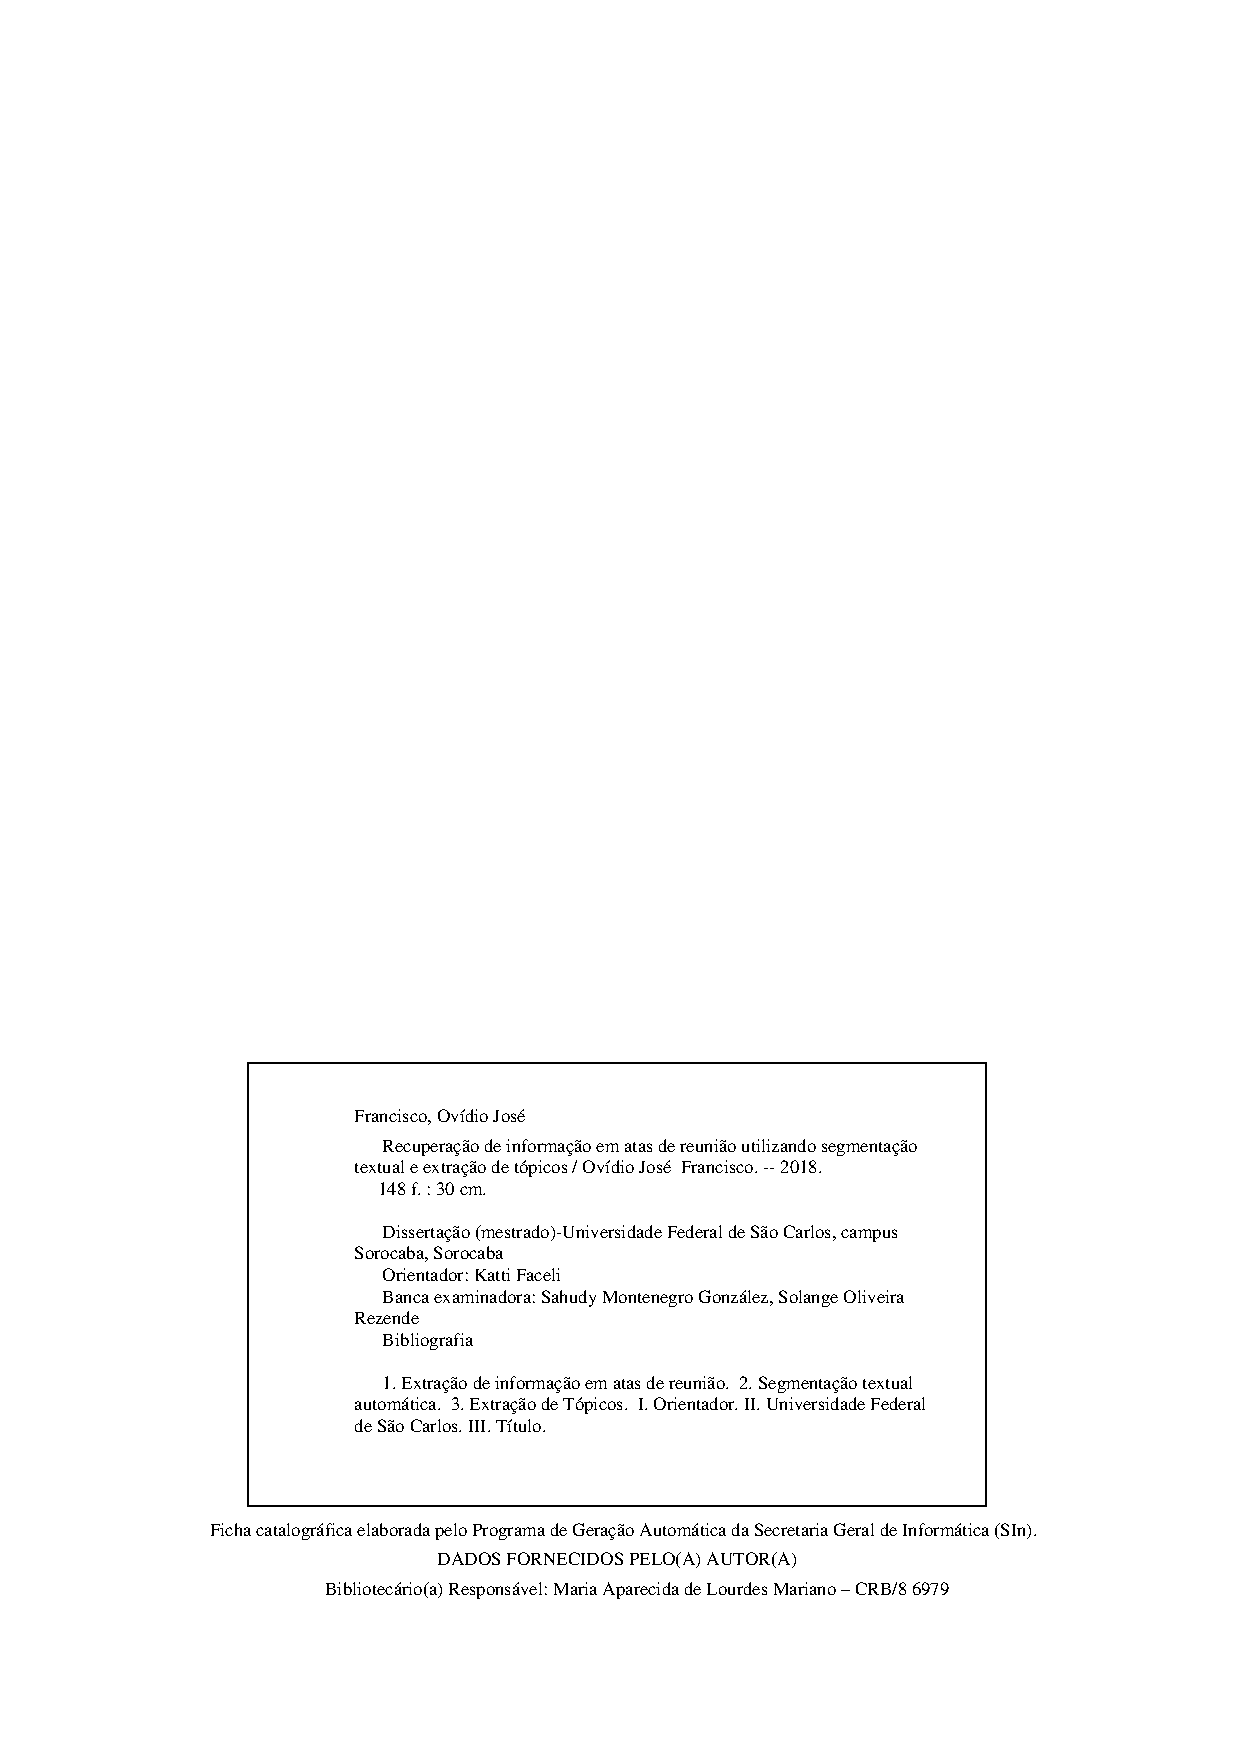
\includepdf{conteudo/fichacatalografica.pdf}
\end{fichacatalografica}

% \begin{fichacatalografica}
	% \vspace*{\fill}					% Posicao vertical
	% \hrule							% Linha horizontal
	% \begin{center}					% Minipage Centralizado
	% \begin{minipage}[c]{12.5cm}		% Largura
	
	% <<Sobrenome>>, <<Nome do aluno>> %Substituir pelos seus dados. Exemplo: Silva, Pedro da
	
	% \hspace{0.5cm} \imprimirtitulo  / \imprimirautor. --
	% \the\year.
	
	% \hspace{0.5cm} \pageref{LastPage} f. : 30 cm.\\
	
	% \hspace{0.5cm}
	% \parbox[t]{\textwidth}{\imprimirtipotrabalho~--~\imprimirinstituicao.\\ \imprimirorientadorRotulo~\imprimirorientador\\
	% Banca examinadora: \imprimirorientador, Prof. Dr. <<Membro 1>>, Prof. Dr. <<Membro 2>>\\
	% Bibliografia}\\

	% \vspace{0.5cm}
	% \hspace{0.5cm}
		% 1. <<Palavra-chave1>>. % Substituir
		% 2. <<Palavra-chave2>>. % Substituir
		% 3. <<Palavra-chave3>>. % Substituir
		% I. Orientador.
		% II. Universidade Federal de S\~{a}o Carlos.
		% III. Título\\ 			
	
	
	% \end{minipage}
	% \end{center}
	% \hrule
% \end{fichacatalografica}
% ---

% ---

% ---
% Inserir folha de aprovacao
% ---
% % Este é um exemplo de Folha de aprovacao, elemento obrigatorio da NBR
% 14724/2011 (secao 4.2.1.3). Voce pode utilizar este modelo ate a aprovacao
% do trabalho. Apos isso, substitua todo o conteudo deste arquivo por uma
% imagem da pagina assinada pela banca com o comando abaixo:
%
% \includepdf{folhaAprovacao_final.pdf}
\includepdf{conteudo/folhadeaprovacao.pdf}
%
% \begin{folhadeaprovacao}

% \vspace*{\fill}

% \begin{center}
% \LARGE\textbf{<<COLOQUE AQUI A CÓPIA DA\\FOLHA DE APROVAÇÃO ASSINADA>>}
% \end{center}

% \vspace*{\fill}
  
% \end{folhadeaprovacao}

% ---

% ---
% Dedicatoria
% ---
% \input{conteudo/3-dedicatoria}
% ---

% ---
% Agradecimentos
% ---
% %======================================= Agradecimentos =======================================
\begin{agradecimentos}

	\vspace{1cm}

\begin{flushright}

	\noindent 
	Agradeço,

Aos meus pais pelo apoio e incentivo aos estudos. 

À Veneranda pela paciência e confiança durante este trabalho. 

Aos professores de toda vida por transmitirem conhecimento e experiência.

E a outros incontáveis familiares e amigos que, cada um à sua maneira, me ajudam até aqui.

\end{flushright}
 
\end{agradecimentos}
%==============================================================================================

% ---

% ---
% Epigrafe
% ---
% %======================================== Epigrafe ===================================
\begin{epigrafe}
    \vspace*{\fill}
	\begin{flushright}
		\textit{``Não há relação de poder sem constituição \\
			correlata de um campo de saber, nem saber \\
		que não suponha e não constitua ao mesmo \\ tempo relações de poder'' \\ (Foucault)}

		% toda forma de saber produz poder
	\end{flushright}
\end{epigrafe}
%==============================================================================================

% ---

% ---
% RESUMOS
% ---
% %================================= Resumo e Abstract ========================================
\setlength{\absparsep}{18pt} % ajusta o espaçamento dos paragrafos do resumo 
                     
% --- 
% resumo em português
% --- 
\begin{resumo}

Em um contexto em que a grande parte das informações armazenadas pelas organizações está em formato textual, o desenvolvimento de ferramentas computacionais para extração de  conhecimento voltadas a organização e recuperação de informação tem se mostrado relevante e recebido atenção.
%
Os modelos de extração de tópicos são recorrentemente empregados nessa tarefa. Esses modelos são capazes de estabelecer relações e encontrar padrões latentes (ocultos) em coleções de documentos textuais.
%
No entanto, há um desafio adicional em documentos constituídos por múltiplos assuntos. Para textos onde há transição de assuntos faz-se necessário, em primeiro lugar, encontrar porções de texto que tratam de um único assunto. Para isso, as técnicas de segmentação textual são utilizada para dividir um texto em segmentos com um assunto relativamente independente.
%
%
%
%
%
% Criação de estrutura. 
O uso combinado de algoritmos de segmentação textual e extração de tópicos pode então ser aplicado para criar uma estrutura que ajuda a entender os dados textuais, os quais são inerentemente não estruturados.
% 
A criação de uma estrutura organizada em tópicos, que incorpora informações latentes sobre o \textit{corpus} favorece as técnicas de recuperação de informação. Essa abordagem permite a extensão do espaço de busca a qual incorpora outros elementos além do conjunto de termos originais de cada segmento, o que favorece a identificação de trechos mais relevantes à consulta.
% 
Neste trabalho, é apresentada uma metodologia para conectar as técnicas de segmentação textual aos modelos de extração de tópicos a fim de gerar uma estrutura derivada de um \textit{corpus} não estruturado. Essa estrutura envolve os textos originais acrescidos de informações latentes e organizadas por sua semelhança semântica.
% 
% 
% 
% 
% 
% 
Assim, a pesquisa deste trabalho de mestrado investigou técnicas de segmentação textual e extração de tópicos para o desenvolvimento de um sistema de recuperação de informação em um conjunto de documentos multi-temáticos, mais especificamente em uma coleção de atas de reunião. 
% 
% Desenvolveu-se uma sistema para entregar ao usuário os segmentos mais relevantes à consulta. 
A ideia desse sistema é entregar os segmentos mais relevantes à consulta do usuário. 
Os segmentos exibidos são agrupados por tópicos. Isso também possibilita consultas exploratórias à base de dados, por meio da navegação por grupos de segmentos relacionados semanticamente. Além disso, trechos pouco relevantes são omitidos, permitindo resultados concentrados no assunto pesquisado.
% 
% 
% 
% 
Para o desenvolvimento do sistema, 
foram avaliados cinco técnicas de segmentação textual e três modelos de extração de tópicos da literatura. Com base no conjunto de atas estudado, criou-se um \textit{corpus} anotado manualmente com informações sobre a composição temática das atas e as transições entre os assuntos. O \textit{corpus} anotado serviu como referência para avaliação objetiva das técnicas de segmentação textual. Avaliou-se ainda, os resultados obtidos com os modelos de extração tópicos junto a profissionais ligados ao contexto de atas de reunião.
% 
% 
% 
% 
Os resultados sugerem que as técnicas utilizadas e a metodologia apresentada entregam respostas satisfatórias. Contudo, mais dados podem ser necessários para execução de novos experimentos a fim de aprimorar os sistema desenvolvido.
% 
% 
% 
% 
% 
% A implementação do sistema e das ferramentas utilizadas, os resultados obtidos nas avaliações, juntamente com o \textit{corpus} anotado, são as principais contribuições deste trabalho no intuito de dar aportes ao desenvolvimento de novos trabalhos.
A implementação do sistema e das ferramentas utilizadas, o corpus anotado, bem como os resultados obtidos nas avaliações são as principais contribuições deste trabalho. 
% 
% 
% 
% 
% 
% criação de um copus anotado mais robusto e 
% bem como avaliações das técnicas utilizadas bem implementação das ferramentas implementadas. 


\textbf{Palavras-chaves}: 
Recuperação de informação. 
Segmentação textual. 
Extração de tópicos.
Atas de reunião.

\end{resumo}
% --- 


% --- 
% resumo em ingl�s
% --- 
\begin{resumo}[Abstract]
 \begin{otherlanguage*}{english}




In a context where the most informations stored by the organizations is in the text format, the development of computer tools for knowledge discovery aimed to organization and information retrieval is a task that holds attention and relevance.
%
The extraction topic models are often employed in this task. This models are able  to establish relations between documents and found latents patterns in sets of them.  
However, there is an additional challenge for documents composed by multiples subjects. For texts with subject shifts, it is necessary, in fist, found the chunks of texts that address a single subject. So, the text segmentation techniques are used to break a text in segments with a relatively independent issue.  
The combination of the text segmentation and topic extraction algorithms, can be used to make an structure that helps to understanding textual data, which are inherently non structured.  
The creation of an topic organized structure, that incorporates latent information concerning the \textit{corpus}, favors Information Retrievals techniques. This approach allows query expansion space, besides the original set of terms of each segment, and the identification most relevant pieces of text.  
This work presents an methodology to connect the Text Segmentation techniques to the Topic extraction models, in order to generates an derivative structure from a non structured \textit{corpus}, which concentrates the original texts plus the latent informations and organized by semantic likeness.  
The research for this thesis investigates the text segmentation techniques and the Topic extraction models to develop an Information Retrieval system for meeting minutes.  
We develops an system to give to the user the most relevant segments to the query. The segmentos presented are clustered by this topics, that also enables exploratory searches to the data base, through browsing by groups of semantically related segments. Furthermore, less relevant segments are omitted, allowing results focused on the researched subject.  
Five techniques of text segmentation and three Topic extraction models from the literature was evaluated. Based on the set of meeting minutes analysed, we create an manually annotated \textit{corpus} with informations on the thematic composition of the meeting minutes and about the issue shifts. The annotated \textit{corpus} served as reference to objective evaluation of the text segmentation techniques. We also evaluate the results obtained with the Topic extraction models. This results were analysed by related to the meeting minutes context.  
The results points the employed techniques and the methodology presented gives satisfactory answers. However, more data can be necessary to leads new experiments in order to improve the used techniques.  
The system implementation and the tools used in the work, as well the results obtained in the evaluations, plus the annotated \textit{corpus} are the principal contributions of this work, in order to support next works.








\textbf{Key-words}: 
% Segmentação Textual. 
% Extração de Tópicos.
% Recuperação de Informação. 
Information retrieval.
Text segmentation.
Topic extraction.
Meeting minutes.
% Dissertation. Text. Master.

 \end{otherlanguage*}
\end{resumo}
% --- 
%===========================================================================================

% ---


%=============================== lista de figuras ==========================
% \pdfbookmark[0]{\listfigurename}{lof}
% \listoffigures*
% \cleardoublepage


%=============================== lista de tabelas ==========================
% \pdfbookmark[0]{\listtablename}{lot}
% \listoftables*
% \cleardoublepage


%====================== lista de abreviaturas e siglas =====================
% \input{conteudo/7-abreviaturas.tex}


%============================ lista de simbolos ============================

%====================== Lista de símbolos ========================


\begin{simbolos}

	\item[$D $]		Conjunto de documentos de uma coleção. 
	\item[$n $]		Número total de documentos em uma coleção.
	\item[$m $]		Número total de termos em uma coleção de documentos.
	\item[$T $]		Conjunto de termos de uma coleção. 
	\item[$t_i $]		i-ésimo termo do vocabulário da coleção de documentos. 
	\item[$w_i $]		Peso i-ésimo termo.
	\item[$ \vec{d} $]	representação vetorial do documento $d$.
	\item[$ q $]		consulta do usuário.
	\item[$ c_i $]		i-ésima sentença da coleção de documentos. 
	\item[$ B $]		Lista de segmentos. 
	\item[$ N $]		Total de sentenças do documento.
	\item[$ Z $]		Conjunto de tópicos. 
	\item[$ z_i $]		i-ésimo tópico do conjunto de tópicos. 

	 
	 
	 
  % \item[$  $]  
  % \item[$  $]  


 
 % $\vec{y}
 
 
 
 
 
 
 
 
 
 
	% \item[$ \Gamma $] Letra grega Gama
	% \item[$ \Lambda $] Lambda
	% \item[$ \zeta $] Letra grega minúscula zeta
	% \item[$ \in $] Pertence
 
 
 
 
 
 
 
 
 
  \end{simbolos}



%==============================================================================================





%=============================== sumario =============================================
\pdfbookmark[0]{\contentsname}{toc}
\tableofcontents*


% ----------------------------------------------------------
% AQUI INICIA OS ELEMENTOS DO TEXTO
% ----------------------------------------------------------
\textual

% \chapter*[Prefácio]{Prefácio}
\addcontentsline{toc}{chapter}{Prefácio}

Dissertação (do latim, \emph{disertatio}), é uma modalidade de redação ou tipo de composição, escrita em prosa sobre um tema que se devem apresentar e discutir argumentos, provas, exemplos etc. Nos meios universitários equivale a tese diferenciando-se pelo volume de material, a dissertação seria o material que envolvesse poucas páginas até o limite de cem, enquanto a tese rotularia os textos que ultrapassassem esse número; e pelo aspecto qualitativo, a dissertação pressupõe a capacidade de aplicação de um método de análise e interpretação, enquanto a tese implica a originalidade do tema ou da abordagem à luz do qual é exposta e discutida (fonte: wikipedia).
\chapter{Introdução}\label{cap1}

\let\cleardoublepage\clearpage


A popularização dos computadores possibilitou o armazenamento cada vez maior de conteúdos digitais, sendo bastante comum, o formato textual como livros, documentos, e-mails, redes sociais e páginas web. A produção de textos gera informações em volumes crescentes que superaram a capacidade humana de análise manual.  % Referências ...
%
Além disso, dados textuais quase sempre apresentam-se em formato não estruturado, caracterizado pela ausência de uma organização pré-definida que facilite a busca em sistemas computacionais.
% para que possam ser recuperados.  % Referências ...
%
Contudo, dados textuais possuem uma organização linguística intrínseca o que possibilita a pesquisa com o uso de ferramentas automáticas para manipulação e consulta a bases dados textuais não estruturadas~\cite{Cao:2017, Manning2008}. 
% Essa dificuldade incentiva a pesquisa de ferramentas automáticas para manipulação e consulta a bases dados textuais não estruturadas~\cite{Cao:2017, Manning2008}. 



Assim, os processos de extração automática de conhecimento em coleções textuais são essenciais, e ao mesmo tempo, constituem um desafio, devido às suas características como o formato não estruturado e trechos com diferentes níveis de importância, desde informações essenciais até textos pouco informativos ou mesmo irrelevantes~
\cite{Aggarwal2012, Jeong:2010, Tagarelli2013}. 
 % -< falar disso mais adiante -->

Além dos tipos de informações mais comuns que são armazenados no formato textual, como e-mails, relatórios, artigos e postagens em redes sociais, têm-se também o armazenamento das atas de reuniões, as quais permitem às organizações a documentação oficial de reuniões em arquivos digitais, facilitando a sua confecção e compartilhamento, bem como consulta às decisões tomadas.
% 
% 
%        ========== ==========   Reuniões   ========== ==========
% 
%Seu conteúdo é frequentemente registrado em texto na forma de atas para fins de documentação e consulta posterior. 
Reuniões são tarefas presentes em ambientes de gestão e organizações de um modo geral, onde discute-se problemas, soluções, propostas, alterações de projetos e frequentemente são tomadas decisões importantes onde a comunicação entre os membros da reunião é feita de forma majoritariamente verbal. 

Para que seu conteúdo possa ser registrado e externalizado, adota-se a prática de escrever seu conteúdo em atas~\cite{Miriam2013, Lee2011}. Por exemplo, nas reuniões do conselho de um programa de pós-graduação de uma universidade, são decididos, quais são os critérios para credenciamento e permanência de docentes no programa. Ao longo do tempo, esse tema pode ser discutido e mencionado diversas vezes, podendo os critérios inclusive passar por significativas alterações, devido a diversos fatores. O coordenador do programa pode desejar recuperar qual foi a decisão mais recente, para poder aplicar os critérios a um potencial novo membro do programa, ou os membros do conselho podem desejar rever o histórico de tudo o que já foi discutido/decidido sobre o tema, para poder propor alterações nas regras, de forma mais adequada.

As atas de reunião possuem características particulares. Frequentemente apresentam um texto com poucas quebras de parágrafo e sem marcações de estrutura, como capítulos, seções ou quaisquer indicações sobre o tema do texto. Devido a fatores como a não estruturação e volume dos textos, a localização de um assunto em uma coleção de atas é uma tarefa custosa, especialmente considerando o seu crescimento de seu número em uma instituição. 
%%  -->


As organizações costumam manter seus documentos eletrônicos organizados em pastas e nomeá-los com informações básicas sobre a reunião a que se refere como a data e alguma referência cronológica, por exemplo \textit{``37ª Reunião Ordinária do Conselho ...''}. Essa organização facilita a localização dos arquivos com ferramentas que fazem buscas pelo nome dos arquivos e pastas, sem levar em conta o teor dos documentos. 
%
Também é comum o uso de ferramentas que fazem buscas nos conteúdos dos documentos, buscando por ocorrências de palavras-chave nos textos. Essas ferramentas permitem buscas combinadas com operadores lógicos como \textit{and}, \textit{or} e \textit{not} ou ainda suporte a expressões regulares. Esse recurso, conhecido como \textit{grepping}\footnote{O nome \textit{grepping} é uma referência ao comando \texttt{grep} do Unix}, produz resultados satisfatórios em muitos casos. Por outro lado, traz algumas desvantagens como: 
1) transfere certa complexidade da tarefa ao usuário 
2) não há suporte a padrões mais flexíveis como a proximidade entre as palavras ou palavras que estejam na mesma sentença 
3) informa apenas se um documento casa ou não com a consulta do usuário com base na presença ou ausência dos termos da consulta~\cite{Aggarwal2012,Manning2008}. 
 

Ainda nesse contexto, usa-se outras técnicas de Recuperação de Informação como o Modelo de Espaço Vetorial para ranquear documentos atribuindo pontuações para a similaridade de cada par documento/consulta. Com isso, é possível apresentar os documentos ordenados conforme a sua relevância com a consulta~\cite{Gutierrez2016, Croft2009, Manning2008}. 
% Utiliza-se também dicionários de sinônimos (\textit{thesaurus}) para expandir a consulta do usuário por meio de conhecimento externo adicionado ao sistema~\cite{X,Y,Z}. % e com isso ...
% TODO: Referências
%
Contudo, essas técnicas baseiam-se na frequência de palavras, em que os documentos e consultas são vistos como conjuntos de termos sem levar em conta relações entre termos que compartilham um mesmo tópico dentro do domínio~\cite{WEIXING}. Por exemplo, as consultas ``\textit{alunos bolsa CAPES}'' e ``\textit{suporte financeiro a pesquisa}'' podem estar relacionados a um assunto em comum,
% tratam de um mesmo assunto, 
nesse caso, a transferência de valores monetários como apoio a carreira acadêmica.
% -> ou ainda "assistência téncina em computadores" e "manutenção de PCs" que tratam de assuntos muito próximos, "conservação de equipamentos de informática".
% -> ou ainda "Workshop desenvolvimento de sites" e "oficina webdesign" que tratam de assuntos muito próximos, "".
Utilizando-se das técnicas até agora mencionadas, obteria-se resultados distintos para cada caso, uma vez que as consultas não compartilham termos e não há relação direta ente eles. Como efeito, os resultados de cada consulta limitariam-se a documentos que compartilham termos com a consulta.
% com termos em comum a consulta.
Essas técnicas produzem resultados melhores a medida que o usuário fornece termos mais acertados na consulta, o que por vezes é dependente de certo conhecimento e familiaridade com o domínio no qual a coleção de documentos está inserida. 
% 
Além disso, o retorno ao usuário é uma lista documentos integrais, o que pode exigir uma segunda busca dentro de um documento para encontrar o trecho desejado.





% Essas técnicas permitem melhorar a busca por informações em atas de reunião~. 
%  Encontra variaveis latentes e agrega informações.
% 
%        ==========   Necessidade de consultas  ==========
% 
Uma vez que a ata registra a sucessão de assuntos discutidos na reunião, um sistema de recuperação de informação idealmente deve retornar ao usuário apenas os trechos que tratem do assunto pesquisado ao invés de documentos inteiros. Assim, cada trecho com um assunto predominate pode ser considerado um subdocumento. Portanto, em primeiro lugar, há a necessidade de descobrir onde há mudanças de assunto no texto. 
% Falar do 'segundo lugar' que é indentificar os tópicos !


% Esse trabalho tem 3 tarefas principais: 
% 1. Segmentar as atas em trechos que tratem de um único assunto.
% 2. Identificar o assunto de cada trecho.
% 3. Ranquear os trechos conforme a relevância com a consulta do usuário.


%        ========== ==========|   Segmentação  |========== ==========

Técnicas de segmentação automática de textos (segmentação textual) podem ser aplicadas com esse propósito. Elas podem dividir um documento em segmentos que contenham um assunto relativamente independente e gerar um conjunto de subdocumentos derivado da coleção de atas original~\cite{Aggarwal2018, bokaei2015a, sakahara2014a, misra2009a, Eis2008}.
%--> onde é usada e como pode ser usada aqui



%        ========== ==========|   Extração de Tópicos  |========== ==========

Contudo, a segmentação textual apenas indica as transições de assuntos ao longo do texto,  sem indicações sobre o teor dos segmentos. O assunto de cada trecho pode ser estimado por meio de modelos de extração de tópicos. Essa técnica possibilita a formação de grupos de segmentos que compartilham o mesmo assunto bem como indicar palavras que melhor descrevem o grupo~\cite{Wei2007}. Com isso, obtém-se uma organização da coleção de documentos que favorece técnicas para navegação e consulta à coleção de documentos~\cite{Maracini2010}. Tais modelos podem eleger um conjunto de termos importantes para um ou mais assuntos, bem como ranquear documentos por sua relevância para determinado tema~\cite{Faleiros2016,Xing2009}.




%        ========== ==========|   Recuperação de Informação  |========== ==========
% ->> RI
% --> tópico é o assunto extraído automaticamente 
% --> segmento é o trecho extraído automaticamente



%        ========== ==========|   Unindo as coisas  |========== ==========

% --> Falando do problema ??
Devido às características das atas, como a multiplicidade de assuntos, e ausência de meta-informação, as técnicas de segmentação podem ser empregadas em conjunto com modelos de extração de tópicos para criar uma estrutura de dados derivada da coleção de documentos original. 
Essa abordagem visa, em primeiro lugar, identificar os assuntos tratados em cada ata e gerar uma coleção de subdocumentos derivados da coleção de atas originais e, a partir disso, utilizar modelos de extração de tópicos para encontrar relações latentes entre os subdocumentos e termos da coleção.
Como resultado, obtém-se uma organização da coleção em que os segmentos são agrupados por assuntos e acrescidos de um conjunto de termos que representam os principais tópicos ou assuntos identificados na coleção de documentos, dessa forma, incorporando conhecimento aos dados originais. Esse novos atributos e a organização das atas por temas podem ser usados para 
% os descrevem, 
% podendo assim 
expandir o espaço de busca a fim de aprimorar técnicas de recuperação de informação em um sistema para extração de conhecimento em coleções de atas de reunião.
% como texto seccionado e \textit{hyperlinks} 



%        ======== ========   Essa abordagem traz como vantagens   ======== ========

Essa abordagem traz vantagens para a recuperação de informação em coleções de documentos com múltiplos tópicos como atas de reunião.
% -> 1 Segmentação
A segmentação das atas permite ao sistema criar uma base de documentos mais simples, em que os assuntos estão isolados em segmentos, formando assim, um \textit{corpus} mais adequado aos métodos de aprendizado de máquina e recuperação de informação, empregados nesse trabalho. Além disso, permite ao sistema final exibir apenas os trechos onde o assunto pesquisado está presente ao invés de entregar documentos integrais~\cite{Tagarelli2013, Jeong:2010, Prince2007, Huang2003}. 

% -> 2 Extração de tópicos -- descritores
Modelos de extração de tópicos podem se integrar ao processo de recuperação de informação usando os agrupamentos e seus descritores como uma forma de descrição da coleção~\cite{Zhai2017, Xing2009}, bem como relacionar termos distintos com um determinado tópico em comum~\cite{WEIXING}. A busca por palavras-chave em descritores transfere esforço computacional da varredura dos documentos para a etapa de extração de tópicos. Essa estratégia evita processamento e lentidão no momento da pesquisa de maneira semelhante à criação de índices para aumentar a eficiência em sistemas de recuperação de informação. Além disso, encontra relações entre termos e documentos sem necessidade de conhecimento externo sobre o domínio. Assim, nesse trabalho os modelos de extração de tópicos são utilizados para incorporar informação aos segmentos com a finalidade de aprimorar o ranqueamento dos resultados~\cite{Maracini2010, WEIXING}. 
% 
% -> 3 Extração de tópicos -- agrupamento
Além disso, ao agrupar os segmentos por tópicos, tem-se uma organização dos documentos que permite a visualização de segmentos semelhantes permitindo a navegação e exploração aos grupos além das consultas por palavras-chave.
%


%        ========== ==========   Objetivos   ========== ==========

Diante desse cenário, o objetivo desse trabalho de mestrado é propor o desenvolvimento uma ferramenta para identificar, organizar e apresentar assuntos registrados em atas de reunião utilizando a estrutura latente de documentos segmentados em conjunto com técnicas de recuperação de informação. 
%
Como objetivos específicos, esse trabalho visa  
% 1)
dar início a investigação de métodos de segmentação textual, extração de tópicos e recuperação de informação no contexto de atas de reunião. Para conhecer a eficiência das técnicas de segmentação textual, seus resultados foram analisados tendo como referência anotações coletadas de profissionais que desempenham atividades ligadas a atas e reuniões.
% 2)
Avaliar junto ao usuário a qualidade dos subdocumentos apresentados quanto ao agrupamento e relevância das informações contidas. Para isso, foi feito uma coleta de dados sobre a percepção de usuários sobre a qualidade dos resultados apresentados em uma consulta a coleção de atas por meio do sistema.
% 
Dessa forma, busca-se ajudar a suprir a necessidade de ferramentas para para esse cenário e contribuindo com uma metodologia de extração de informação em documentos com múltiplos assuntos. Além disso, disponibilizar o sistema implementado bem como os dados coletados durante a análise das técnicas de forma a contribuir com novos trabalhos relacionados a esse contexto.

% --> Disponibilisação do sistema final.



% \section{Organização da Dissertação}

No Capítulo~\ref{cap2} são apesentados os principais conceitos da Recuperação de Informação, de Mineração de Textos, Segmentação Textual e Extração de Tópicos.
%
No Capítulo~\ref{cap3} é proposto um sistema para extração de conhecimento em atas de reunião e inicia-se o seu desenvolvimento com base nas técnicas mencionadas. 
Ainda nesse capítulo, é mostrado um estudo de caso da aplicação das técnicas de Segmentação Textual e Extração de Tópicos em uma coleção de atas. 
%
No Capítulo~\ref{cap-segmentadores} é apresentada uma avaliação objetiva em algoritmos de Segmentação Textual a fim de analisar seus resultados e escolher um segmentador a ser utilizado no sistema proposto.
anotações
%
No Capítulo~\ref{cap-extratores} é apresentada uma avaliação subjetiva dos resultados dos modelos de Extração de Tópicos sob um \textit{corpus} composto por segmentos de atas. Adicionalmente, avaliou-se o segmentador utilizado, uma vez que este está ligado aos resultados avaliados. 
%
Por fim as conclusões do trabalho, as limitações dessa pesquisa e os trabalhos futuros são apresentados no último capítulo dessa dissertação.





% "Diante do cenário descrito na seção anterior, a hipótese levantada neste trabalho é que a qualidade da recomendação é melhorada quando são utilizadas hierarquias de tópicos como informações contextuais."











% // https://verbosus.com/bibtex-style-examples.html

\chapter{Conceituação Teórica}\label{cap2}



A popularidade dos computares permite a criação e compartilhamento de textos onde a quantidade de informação facilmente extrapola a capacidade de humana de leitura e análise de coleções de documentos, estejam eles disponíveis na Internet ou em computadores pessoais. A necessidade de simplificar e organizar grandes coleções de documentos criou uma demanda por modelos de aprendizado de máquina para extração de conhecimento em bases textuais. Para esse fim, foram desenvolvidas técnicas para descobrir, extrair e agrupar textos de grandes coleções, entre essas, a modelagem de tópicos~\cite{Hofmann1999,Deerwester1990,Lee1999,Blei2012}.  %--> não falar só de modelagem de tópicos. Falar de RI com referências


\section{Conceitos Básicos}
% Nesse trabalho, são utilizadas técnicas comuns da área da computação, por exemplo a medida \textit{cosseno} é amplamente utilizada para mensurar a similaridade entre objetos. 

% -> Representação de Textos
\subsection*{Representação de Textos} 
\label{section:RepTextos}

Os dados textuais se diferenciam de outros formatos estruturados como bancos de dados relacionais em que um dado é facilmente encontrado. Uma das etapas mais importantes para as tarefas de Mineração Textos é a criação de uma representação adequada dos dados. Essa representação deve prover uma maneira estruturada para que os textos possam ser processados e utilizados por algoritmos de Aprendizado de Máquina. 




Uma das formas mais comuns para que a grande maioria dos algoritmos possa extrair padrões das coleções de textos é a representação no formato matricial conhecido como Modelo Espaço Vetorial (\textit{Vectorial Space Model} - VSM)~\cite{Rezende2003}, onde os documentos são representados como vetores em um espaço Euclidiano $m$-dimensional em que cada termo extraído da coleção é representado por uma dimensão. Assim, cada componente de um vetor expressa a relação entre os documentos e as palavras. Essa estrutura é conhecida como matriz documento-termo (\textit{document-term matrix}). Uma das formas mais populares dessa matriz é conhecida como \textit{Bag Of Words} a qual é detalhada a seguir.
	

\subsection*{\textit{Bag Of Words}}
% \subsection{\textit{Bag Of Words}} \label{subsubsec:BOW}
		
Nessa representação, cada termo é transformado em um atributo  (\textit{feature}), em que $a_{ij}$ é o peso do termo $t_j$ no documento $d_i$ e indica a sua relevância dentro da base de documentos. As medidas mais tradicionais para o cálculo desses pesos são a binária, onde o termo recebe o valor 1 se ocorre em determinado documento ou 0 caso contrário; \textit{document frequency}, que é o número de documentos no qual um termo ocorre; \textit{term frequency - tf}, atribui-se ao peso a frequência do termo dentro de um determinado documento; \textit{term frequency-inverse document frequency, tf-idf}, pondera a frequência do termo pelo inverso do número de documentos da coleção em que o termo ocorre.
Essa representação é mostrada pela Tabela \ref{table:bagofwords}.

\begin{table}[!h]
	\centering

	\begin{tabular}{|c|ccccc|}

	\hline
	    & $t_1$      & $t_2$     & $t_j$    & \dots & $t_m$      \\ \hline \hline
	$d_1$ & $a_{11}$ & $a_{12}$  & $a_{1j}$ & \dots & $a_{1m}$   \\  %\hline 
	$d_2$ & $a_{21}$ & $a_{22}$  & $a_{2j}$ & \dots & $a_{2m}$   \\  %\hline 
	$d_i$ & $a_{i1}$ & $a_{i2}$  & $a_{ij}$ & \dots & $a_{im}$   \\  %\hline 
	\vdots & \vdots    & \vdots     & \vdots    & \ddots & \vdots      \\  %\hline 
	$d_n$ & $a_{n1}$ & $a_{n2}$  & $a_{nj}$ & \dots & $a_{nm}$   \\  \hline 

	\end{tabular}

	\caption{Coleção de documentos na representação \textit{bag-of-words}}
	\label{table:bagofwords} 
\end{table}


Essa forma de representação sintetiza a base de documentos em um contêiner de palavras, ignorando a ordem em que ocorrem, bem como pontuações e outros detalhes, preservando apenas o peso de determinada palavra nos documentos. É uma simplificação de toda diversidade de informações contidas na base de documentos sem o propósito de ser uma representação fiel do documento, mas oferecer a relação entre as palavras e os documentos a qual é suficiente para a maioria dos métodos de Aprendizado de Máquina~\cite{Aggarwal2018, Feldman2006, Rezende2003}. 






% (Manning et al., 2008; Feldman e Sanger, 2006) Tese Rafael		




\subsection{Medidas de Proximidade}
% -- Movido para "Medidas de Proximidade " ↓↓↓↓
No modelo espaço vetorial, a similidade entre um documentos $x$ e $y$ é calculada pela correlação entre os vetores $\vec{x}$ e $\vec{y}$, a qual pode ser medida pelo cosseno do  ângulo entre esses vetores. Dados dois documentos $x = (x_1, x_1, \dots, x_t)$ e $y = (y_1, y_1, \dots, y_t)$, calcula-se: 


% conforme mostrado na Equação~\ref{equ:cosseno-doc-consulta}.


\begin{equation}
cosseno(x, y) = \frac{ \vec{x} \bullet \vec{y} }
                   { |\vec{x}| \times | \vec{y}|}
            = \frac{ \sum_{i=1}^{t} x_i \cdot y_i}
                   { \sqrt{\sum_{i=1}^{t} x_i^2} \times \sqrt{\sum_{i=1}^{t} y_i^2 } }                   \label{equ:cosseno-doc-consulta}		                   
\end{equation} 

aa
Valores de cosseno próximos a 0 indicam um ângulo próximo a 90º entre $\vec{x}$ e $\vec{y}$, ou seja, o documento $x$ compartilha poucos termos com a consulta $y$, enquanto valores próximos a 1 indicam um ângulo próximo a 0º, ou seja, $x$ e $y$ compartilham termos e são similares~\cite{Tan2005,Feldman2006}.


% -> Medidas utilizadas nessa dissertação
\documentclass{article} 
\begin{document} 
\begin{tabular}{|l|c|c|c|c|c|c|} 
\hline 
Configuração & \textbf{Pk} & \textbf{WD} & \textbf{A } & \textbf{P } & \textbf{R } & \textbf{F1}\\ \hline
TextTiling 20  3 T & 0.272 & 0.481 & 0.519 & 0.511 & \textbf{0.917} & 0.630\\ \hline
TextTiling 20  6 T & 0.232 & 0.477 & 0.523 & 0.521 & 0.738 & 0.584\\ \hline
TextTiling 20  9 T & 0.157 & 0.421 & 0.579 & 0.571 & 0.675 & 0.594\\ \hline
TextTiling 20 12 T & 0.159 & 0.466 & 0.534 & 0.541 & 0.504 & 0.497\\ \hline
TextTiling 30  3 T & 0.258 & 0.464 & 0.536 & 0.518 & 0.874 & 0.627\\ \hline
TextTiling 30  6 T & 0.229 & 0.465 & 0.535 & 0.526 & 0.730 & 0.588\\ \hline
TextTiling 30  9 T & 0.161 & 0.462 & 0.538 & 0.531 & 0.574 & 0.531\\ \hline
TextTiling 30 12 T & 0.143 & 0.491 & 0.509 & 0.510 & 0.446 & 0.452\\ \hline
TextTiling 40  3 T & 0.203 & 0.406 & 0.594 & 0.566 & 0.843 & 0.649\\ \hline
TextTiling 40  6 T & 0.222 & 0.469 & 0.531 & 0.525 & 0.630 & 0.551\\ \hline
TextTiling 40  9 T & 0.134 & 0.396 & 0.604 & 0.618 & 0.580 & 0.571\\ \hline
TextTiling 40 12 T & 0.159 & 0.452 & 0.548 & 0.561 & 0.451 & 0.475\\ \hline
TextTiling 50  3 T & 0.202 & 0.442 & 0.558 & 0.547 & 0.748 & 0.604\\ \hline
TextTiling 50  6 T & 0.168 & 0.469 & 0.531 & 0.552 & 0.532 & 0.511\\ \hline
TextTiling 50  9 T & 0.144 & 0.453 & 0.547 & 0.579 & 0.479 & 0.494\\ \hline
TextTiling 50 12 T & 0.148 & 0.427 & 0.573 & 0.614 & 0.456 & 0.491\\ \hline
TextTiling 60  3 T & 0.166 & 0.420 & 0.580 & 0.576 & 0.729 & 0.614\\ \hline
TextTiling 60  6 T & 0.160 & 0.441 & 0.559 & 0.574 & 0.511 & 0.518\\ \hline
TextTiling 60  9 T & 0.152 & 0.428 & 0.572 & 0.601 & 0.487 & 0.510\\ \hline
TextTiling 60 12 T & 0.150 & 0.424 & 0.576 & 0.611 & 0.472 & 0.499\\ \hline
C99 20  9 false T & 0.129 & 0.452 & 0.548 & 0.669 & 0.226 & 0.326\\ \hline
C99 20  9 true T & 0.127 & 0.465 & 0.535 & 0.618 & 0.216 & 0.308\\ \hline
C99 20 11 false T & \textbf{0.116} & 0.434 & 0.566 & \textbf{0.721} & 0.255 & 0.363\\ \hline
C99 20 11 true T & 0.119 & 0.455 & 0.545 & 0.651 & 0.237 & 0.333\\ \hline
C99 30  9 false T & 0.155 & 0.477 & 0.523 & 0.542 & 0.302 & 0.373\\ \hline
C99 30  9 true T & 0.134 & 0.459 & 0.541 & 0.572 & 0.333 & 0.404\\ \hline
C99 30 11 false T & 0.142 & 0.459 & 0.541 & 0.574 & 0.331 & 0.404\\ \hline
C99 30 11 true T & 0.126 & 0.449 & 0.551 & 0.590 & 0.354 & 0.424\\ \hline
C99 40  9 false T & 0.163 & 0.456 & 0.544 & 0.562 & 0.428 & 0.467\\ \hline
C99 40  9 true T & 0.155 & 0.438 & 0.562 & 0.585 & 0.454 & 0.489\\ \hline
C99 40 11 false T & 0.156 & 0.443 & 0.557 & 0.578 & 0.448 & 0.484\\ \hline
C99 40 11 true T & 0.142 & 0.426 & 0.574 & 0.601 & 0.473 & 0.506\\ \hline
C99 50  9 false T & 0.161 & 0.430 & 0.570 & 0.570 & 0.582 & 0.557\\ \hline
C99 50  9 true T & 0.147 & 0.400 & 0.600 & 0.601 & 0.628 & 0.593\\ \hline
C99 50 11 false T & 0.146 & 0.407 & 0.593 & 0.594 & 0.622 & 0.587\\ \hline
C99 50 11 true T & 0.156 & 0.410 & 0.590 & 0.590 & 0.614 & 0.581\\ \hline
C99 60  9 false T & 0.202 & 0.457 & 0.543 & 0.534 & 0.643 & 0.564\\ \hline
C99 60  9 true T & 0.164 & \textbf{0.390} & \textbf{0.610} & 0.592 & 0.736 & 0.633\\ \hline
C99 60 11 false T & 0.189 & 0.439 & 0.561 & 0.550 & 0.673 & 0.584\\ \hline
C99 60 11 true T & 0.169 & 0.400 & 0.600 & 0.583 & 0.722 & 0.623\\ \hline
C99 70  9 false T & 0.204 & 0.452 & 0.548 & 0.532 & 0.757 & 0.603\\ \hline
C99 70  9 true T & 0.191 & 0.409 & 0.591 & 0.563 & 0.816 & 0.643\\ \hline
C99 70 11 false T & 0.204 & 0.431 & 0.569 & 0.548 & 0.788 & 0.623\\ \hline
C99 70 11 true T & 0.189 & 0.416 & 0.584 & 0.558 & 0.803 & 0.635\\ \hline
C99 80  9 false T & 0.227 & 0.443 & 0.557 & 0.535 & 0.870 & 0.638\\ \hline
C99 80  9 true T & 0.220 & 0.423 & 0.577 & 0.547 & 0.897 & 0.655\\ \hline
C99 80 11 false T & 0.233 & 0.448 & 0.552 & 0.531 & 0.862 & 0.634\\ \hline
C99 80 11 true T & 0.220 & 0.421 & 0.579 & 0.548 & 0.898 & \textbf{0.656}\\ \hline
\end{tabular} 
\end{document} 
 




% -> Segmentação 
\documentclass[12pt]{article}

\usepackage{sbc-template}

\usepackage{graphicx,url}

%\usepackage[brazil]{babel}   
\usepackage[latin1]{inputenc}  

%\usepackage{subfig}
\usepackage{subfigure}
     
\sloppy

\title{Segmenta��o Textual Autom�tica de Atas de Reuni�o}

%\author{Luciana P. Nedel\inst{1}, Rafael H. Bordini\inst{2}, Fl�vio Rech Wagner\inst{1}, Jomi F. H�bner\inst{3} }


\address{%Instituto de Inform�tica -- Universidade Federal do Rio Grande do Sul (UFRGS)\\  Caixa Postal 15.064 -- 91.501-970 -- Porto Alegre -- RS -- Brazil
%\nextinstitute
%  Department of Computer Science -- University of Durham\\
%  Durham, U.K.
%\nextinstitute
%  Departamento de Sistemas e Computa��o\\
%  Universidade Regional de Blumenal (FURB) -- Blumenau, SC -- Brazil
%  \email{\{nedel,flavio\}@inf.ufrgs.br, R.Bordini@durham.ac.uk,
%  jomi@inf.furb.br}
}




\newcommand{\urlatas}{http://www.ppgccs.net/?page\_id=1150}

\newcommand{\urlbrowcorpus}{http://clu.uni.no/icame/brown/bcm.html}
\newcommand{\urlreuterscorpus}{http://trec.nist.gov/data/reuters/reuters.html}
\newcommand{\urlicsi}{http://www1.icsi.berkeley.edu/Speech/mr}
% LDC -- Linguistic Data Consortium
\newcommand{\urltdt}{https://catalog.ldc.upenn.edu/LDC98T25}
\newcommand{\urlwsj}{https://catalog.ldc.upenn.edu/ldc2000t43}
\newcommand{\urlcaloproject}{http://www.ai.sri.com/project/CALO}
\newcommand{\urlami}{http://groups.inf.ed.ac.uk/ami/corpus}

\newcommand{\urlorengo}{http://www.inf.ufrgs.br/~viviane/rslp/}



\usepackage[linesnumbered,ruled,portuguese]{algorithm2e}

% Define o caminho das figuras
\graphicspath{{images/}}


\begin{document} 

\maketitle

\begin{abstract}


A tarefa de segmentação topical consiste em dividir um texto em porções com significado relativamente independente, de maneira que cada segmento contenha um assunto. 
%
%
A segmentação de atas de reuniões é útil na organização desses documentos e para facilitar o seu acesso.
%
%
Este artigo traz uma revisão bibliográfica dos métodos segmentação textual e se concentra nos algoritmos mais influentes adaptando-os ao contexto das atas de reunião em português, bem como a encontrar um modelo que ofereça segmentos coesos e contribua a sistemas de recuperação de informação para que respondam melhor à buscas do usuário.
%
%
Para a avaliação, um conjunto de atas foi manualmente segmentado por participantes das reuniões, então comparou-se as divisões manuais com as geradas automaticamente. Os testes registraram precisão de 0.7106, revocação de 0.8516, as medidas P$_k$ e \textit{WindowDiff} mostram respectivamente 0.1163 e 0.3800 de dissimilaridade.





% na adaptação dos algoritmos mais influentes ao contexto das atas de 

%a fim de melhor responder a buscas do usuário em sistemas de recuperação de informação.

%divida um documento em partes .



% os influentes tratam muito de discursos e textos longos
% as atas apresentam texto mais enxuto/compacto e com estilo próprio.
% as atas são uma paráfrase da reunião

\end{abstract}

	Frequentemente atas de reunião tem a característica de apresentar um texto com poucas quebras de parágrafo e sem marcações de estrutura, como capítulos, seções ou quaisquer indicações sobre o tema do texto. 


% Definição 

A tarefa de segmentação textual consiste dividir um texto em partes que contenham um significado relativamente independente. Em outras palavras, é identificar as posições onde há uma mudança significativa de tópicos.

% Usos
É útil em aplicações que trabalham com textos sem quebras de assunto, ou seja, não apresentam parágrafos, seções ou capítulos, como transcrições automáticas de áudio e grandes documentos que contêm assuntos não idênticos como atas de reunião e noticias.


% Interesses
O interesse por segmentação textual tem crescido em em aplicações voltadas a recuperação de informação %citar o [15] ...
e sumarização de textos. % ... e [2] do "Efficient Linear T S"
Essa técnica pode ser usada para aprimorar o acesso a informação quando essa é solicitada por um usuário por meio de uma consulta, onde é possível oferecer porções menores de texto mais relevante ao invés de exibir um documento maior que pode conter informações menos pertinente. A sumarização de texto também pode ser aprimorada ao processar segmentos separados por tópicos ao invés de documentos inteiros.




% As Atas
Assim, esse trabalho trata da adaptação e avaliação de algoritmos tradicionais ao contexto de documentos em português do Brasil, com ênfase especial nas atas de reuniões.


%As atas, como frequentemente são, apresentam-se como uma sucessão de tópicos. Assim, o objetivo desse trabalho é identificar, automaticamente, onde há a mudança de um tópico para seus adjacentes.


% Diversas aplicações fazem uso de segmentação textual, incluindo 

% Entre as principais mais frequentes de segmentação textual estão a tra



%É principalmente utilizada em aplicações que processam textos longos como transcrições de áudio e documentos longos, além de aprimorar técnicas de sumarização e information retrievel.



% Usos:
%	* quando não há identificações
%	* em transcrições de áudio
%	* em documentos longos
% 	* text summarization (ver a referencia [2] de Efficient Linear Text...)




%Isto é, dado um texto, identificar onde há mudança de tópicos.


% Interest in automatic text segmentation has blossomed over the last few years, with applications ranging from information retrieval to text summariza-tion to story segmentation of video feeds. [A Critique and Improvement of an Evaluation Metric for Text Segmentation]



%Em outras palavras é identificar divisões entre unidade de informação sucessivas

%A tarefa de segmentação textual consiste em encontrar pontos onde há mudança de tópicos no texto.



%[ The task of linear text segmentation is to split a large text document into shorter fragments, usually blocks of consecutive sentences. ]


% **Segmentação é identificar divisiões entre unidades de informação sucessivas (Beeferman, Berger, and Lafferty (1997))**

%   [Text segmentation is the task of determining the positions at which topics change in a stream of text]





	\section{Referencial Teórico}
	\label{sec:referencial}
	
%%%%%%%%%%
% Retomada das Definições
%%%%%%%%%%	

Um documento textual, sobre tudo quando longo, é frequentemente uma sucessão de tópicos. 
%%%%%%%%%%
% Segmentação
%%%%%%%%%%
A segmentação textual ou segmentação topical é a tarefa de dividir um texto mantendo em cada parte um tópico com seu significado completo.
	
%%%%%%%%%%
% Segmento
%%%%%%%%%%	
Um segmento pode ser visto como uma sucessão de unidades de informação que compartilham um tópico essas unidades podem ser, por exemplo, palavras, sentenças ou parágrafos. Sendo a menor parte de um segmento, portanto são consideradas candidatas a limite entre segmentos.

%%%%%%%%%%
% Coesão léxica como **presuposto básico**
%%%%%%%%%%
Trabalhos anteriores se apoiam na ideia de que a mudança de tópicos em um texto é acompanhada de uma proporcional mudança de vocabulário, essa ideia, chamada de coesão léxica, sugere que a distribuição das palavras é um forte indicador da estrutura do texto. A partir disso, vários algoritmos foram propostos baseados na ideia de que um segmento pode ser identificado e delimitado pela análise das palavras que o compõe~\cite{Galley2003}~\cite{Boguraev2000}.



%, bem como é necessário mensurar suas similaridades. { asunidades de medida}

%%%%%%%%%%
% Porque cosseno
%%%%%%%%%%
Uma vez que a coesão léxica é pressuposto básico da maioria dos algoritmos, o cálculo da similaridade entre unidades de informação (comumente sentenças) é fundamental. Uma medida de similidade frequentemente utilizada é o cosseno, a qual pode ser vista na Equação~\ref{equ:cosine}, sendo $f_{x,j}$ a frequência da palavra $j$ na sentença $x$ e $f_{y,j}$ sendo a frequência da palavra $j$ na sentença $y$.


\begin{equation}
Sim(x,y) = \frac
{\Sigma_j f_{x,j} \times f_{y,j}}
{\sqrt{\Sigma_j f^2_{x,j} \times \Sigma f^2_{y,j}}}
\label{equ:cosine}
\end{equation}


\subsection{Principais algoritmos}
	\label{subsec:principaisalgoritimos}

Entre os principais trabalhos da literatura podemos citar o  \textit{TextTiling}~\cite{Hearst1994} e o \textit{C99}~\cite{Choi2000}, os quais são mostrados a seguir.

%%%%%%%%%%%%%%%%%%%%%%%%%%%%%%%%%%%%%%%%%%%%%%%
%%%              TextTiling                 %%%
%%%%%%%%%%%%%%%%%%%%%%%%%%%%%%%%%%%%%%%%%%%%%%%
O \textit{TextTiling} é um algoritmo baseado em janelas deslizantes, onde para cada candidato a limite, analisa-se o texto circundante. Um limite ou quebra de segmento é identificado quando a similaridade entres os blocos apresenta uma queda considerável.

%Ela propõe um algoritmo baseado em janelas deslizante, para analisar blocos de texto adjacentes e identificar os limites com base nas similaridades dos blocos.

O \textit{TextTiling} recebe uma lista de candidatos a limite, usualmente finais de parágrafo ou finais de sentenças. Para cada posição candidata são construídos 2 blocos, um contendo sentenças que a precedem e outro com as que a sucedem. O tamanho desses blocos é um parâmetro a ser fornecido ao algoritmo e determina o tamanho mínimo de um segmento.
%
Em seguida, os blocos de texto são representados por vetores que contém as frequências de suas palavras. Então, usa-se cosseno (Equação~\ref{equ:cosine}) para calcular a similaridade entre os blocos adjacentes a cada candidato e identifica-se uma transição entre tópicos pelos picos na curva se dissimilaridade.

%TODO como apresentado na Figura~\ref{fig:curvadedissimilaridade}.

%sempre que a similaridade cai abaixo de um \textit{threshold}.

O \textit{TextTiling} apresenta baixa complexidade computacional, devido a simplicidade do algoritmo e baixa eficiência quando comparado a outros métodos mais sofisticados como apresentados em~\cite{Choi2000, Kern2009, Misra2009}.



%%%%%%%%%%%%%%%%%%%%%%%%%%%%%%%%%%%%%%%%%%%%%%%
%%%                  C99                    %%%
%%%%%%%%%%%%%%%%%%%%%%%%%%%%%%%%%%%%%%%%%%%%%%%

Choi \cite{Choi2000} apresenta um esquema de ranking em seu algoritmo, o \textit{C99}. 
%
Embora muitos trabalhos utilizem matrizes de similaridades, o autor traz obervações.
%
Ele aponta que para pequenos segmentos, o cálculo de suas similaridades não é confiável, pois uma ocorrência adicional de uma palavra causa um impacto desproporcional no cálculo.
%
Além disso, o estilo da escrita pode não ser constante em todo o texto. Choi sugere que, por exemplo, textos iniciais dedicados a introdução costumam apresentar menor coesão do que trechos dedicados a um tópico específico. 
%

Portanto, comparar a similaridade entre trechos de diferentes regiões, não é apropriado.
% Complexidade O(n²)
Devido a isso, as similaridades não podem ser comparadas em valores absolutos. Então, o autor apresenta um esquema de \textit{rankings} para contornar esse problema.


%

% 1 cria uma matrix de similaridades
% 2 cria a matrix de ranking
% 3 aplica divisive clustering

% mask = quadro
% pegar um exemplo --> mostrar os numeros dentro do quatro e pq o resultado foi aquele

% colocar os passos na imagem


Inicialmente é construída uma matriz que contém as similaridades de todas as unidades de texto. Em seguida, cada valor na matriz de similaridade é substituído por seu ranking local. Onde para cade elemento da matiz, seu \textit{ranking} é o número de elementos vizinhos com valor de similaridade menor ao seu.%, o qual é calculado com a Equação~\ref{equ:ranklocal}. 

Na Figura~\ref{fig:exemplomatrixrank} vemos um quadro de dimensões 3~x~3 destacado na matriz de similaridades, que contém os valores  $\{0,3; 0,4; 0,4; 0,6; 0,5; 0,2; 0,9; 0,5; 0,7\}$, tomando como exemplo o elemento com valor $0,5$, a mesma posição na matriz de \textit{ranks} terá o valor $4$, pois esse é número de vizinhos com valores inferiores a $0,5$ dentro do quadro analisado na matriz de similaridades. 


%nesse exemplo, o valor $0,5$ é substituído por $4$ na matriz de ranks pois há 4 vizinhos com valor inferior

%o valor $0,5$ é comparado com seus elementos vizinhos, o


%Um exemplo é mostrado na Figura \ref{fig:exemplomatrixrank} abaixo, onde utiliza-se uma máscara de largura igual a 3.



  \begin{figure}[!h]

	\centering
	\includegraphics[width=0.45\textwidth]{exemplo-matrix-rank-noborder.jpg}
	\caption{Exemplo de construção de uma matriz de rank.~\cite{Choi2000}}
	\label{fig:exemplomatrixrank}

  \end{figure}




%\begin{equation}
%r(x,y) = \frac
%{Numero\ de\ elementos\ com\ similaridade\ menor}
%{Numero\ de\ elementos\ examinados}
%\label{equ:ranklocal}
%\end{equation}


% Clustering Reynar maximization
	
Finalmente, utiliza um método de divisão por \textit{clustering} baseado no algoritmo de maximização de Reynar~\cite{Reynar1998} para identificar os limites entre os segmentos. %Essa abordagem apresenta uma redução taxa de erros de 22\% para 10\%. Por outro lado, exige que a quantidade de segmentos seja conhecida.
%Como melhoramento, os autores apresentam posteriormente uma versão do \textit{C99} que utiliza \textit{Latent Semantic Analisys} (LSA) para calcular as similaridades ao invês de cosseno~\cite{Choi2001-LSA}.




\subsection{Medidas de Avaliação}

%%%%%%%%%%
%	Avaliações baseadas em hits 
%%%%%%%%%%

As medidas de avaliação tradicionais, baseiam se na contagem de acertos. No contexto da segmentação de textos um acerto é quando um o limite hipotético coincide com um limite de referência.

Essas medidas de avaliação tentam computar os erros do algoritmo, isto é falsos positivos e falsos negativos, a fim de calcular sua eficiência. 
%
% falso positivo
Um falso positivo é um limite identificado pelo algoritmo que não corresponde a nenhum limite na segmentação de referência. 
%
% falso negativo
Um falso negativo é quando o algoritmo não identifica um limite existente na segmentação de referência.


Nesse sentido, 
%
a precisão, que é a proporção de limites corretamente identificados pelo algoritmo, e 
%
a revocação, que é a proporção de limites verdadeiros que foram identificados pelo algoritmo,
%
trazem alguns problemas na avaliação de segmentadores automáticos.
 	
	
Conforme o algoritmo aponta mais segmentos no texto, este tende a melhorar a revocação e ao mesmo tempo, reduzir a precisão. Esse problema de avaliação pode ser contornado utilizado a medida F-1 que é uma média harmônica entre precisão e revocação onde ambas tem a o mesmo peso. Por por outro lado, tem a desvantagem de ser mais difícil de interpretar. 

As medidas apresentadas acima falham ao não serem sensíveis a \textit{near misses}, ou seja, quando um limite não coincide exatamente com o esperado, mas está próximo a ele~\cite{Kern2009}.

Na Figura~\ref{fig:exemplosegmentacaozoom} é apresentado um exemplo com duas segmentações hipotéticas e uma referência. Na Figura~\ref{fig:exemplosegmentacao}, em ambos os casos não há nenhum verdadeiro positivo, o que implica em zero para os valores de precisão, acurácia, e revocação, embora a segunda hipótese possa ser considerada superior à primeira se levado em conta a proximidade dos limites.



  \begin{figure}[!h]

	\centering
	\includegraphics[width=0.47\textwidth]{windiffzoom.jpg}
	\caption{Exemplos de \textit{near missing} e falso positivo puro. Os blocos indicam uma unidade de informação e as linha verticais representam os limites entre segmentos de texto representando um tópico do texto. }
	\label{fig:exemplosegmentacaozoom}

  \end{figure}
  
  \begin{figure}[!h]

	\centering
	\includegraphics[width=0.47\textwidth]{windiff.jpg}
	\caption{
	Exemplo de duas segmentações hipotéticas em comparação a uma ideal. 
	}
	\label{fig:exemplosegmentacao}

  \end{figure}
  
  
Entre as medidas mais utilizadas para avaliar segmentadores estão:

\begin{enumerate}

	\item P$_k$. A fim de resolver o problema de \textit{near misses}, Beeferman \textit{et. al.}~\cite{Beeferman1999} apresentam uma medida chamada P$_k$ que atribui 
%
valores parciais a \textit{near misses}, 
%
ou seja, limites sempre receberão um peso proporcional à sua proximidade, desde que dentro de um janela de tamanho~$k$.
%
Para isso, esse método move uma janela de tamanho $k$ e a cada posição e verifica se o início e o final da janela estão ou não dentro do mesmo segmento e penaliza o algoritmo em caso de discrepância. Ou seja, dado duas palavras de distancia $k$, uma discrepância é computada quando o algoritmo e a referência não concordam se as palavras estão ou não no mesmo segmento.

O valor de $k$ é calculado como a metade da média dos comprimentos dos segmentos reais. Como resultado, é retornado a contagem de discrepâncias divido pelo quantidade de segmentações analisadas. Esse valor serve como medida de dissimilaridade entre as segmentações e pode ser interpretada como a probabilidade de duas sentenças extraídas aleatoriamente pertencerem ao mesmo segmento.

\item \textit{WindowDiff}. Pevzner~\cite{Pevzner2002} aponta problemas na avaliação mais tradicional, P$_k$~\cite{Beeferman1999}. Eles apontam que esse método penaliza demasiadamente os falsos negativos em relação aos falsos positivos e a \textit{near misses}, além disso, desconsidera o tamanho dos segmentos. Como solução, propõem um método, que traz duas diferenças principais: a dobra da penalidade para os falsos positivos a fim de diminuir o problema da subestimação dessa medida e, diferente de P$_k$, ao mover a janela pelo texto, penaliza-se o algoritmo sempre que o número de limites proposto pelo algoritmo não coincidir com o número de limites esperados para aquela janela de texto. 

Com isso, demonstram em seu trabalho que, em relação a P$_k$, consegue resolver seus principais problemas e mantém sua proposta inicial de sensibilidade a \textit{near misses}, penalizando-os menos que os falsos positivos puros.


\end{enumerate}














%apontam que a coesão léxica é um forte indicador da estrutura do texto, isto é, a mudança de tópicos é acompanhada de uma proporcional mudança de vocabulário. A partir disso, vários algoritmos foram propostos baseados na ideia de que um segmento pode ser identificado e delimitado pela análise das palavras que o compõe~\cite{Galley2003}~\cite{Boguraev2000}.


%Finalmente, os limites são identificados sempre que a similaridade entre blocos adjacentes entre cada candidato ultrapassa um determinado \textit{threshold}.



% Mensionar que existem duas abordagens principais - Baseada em coesão léxiam e em discursos [ver a pg 2 do Text Segmentation With Topic Moeling and Entity Coherence]




%Há ainda outros critérios para segmentação como a segmentação temática 

%outros tipos de abordagem
%	Segmentação funcional
%	Segementação temática
	
	% Ideia básica dos algorítmos (Coesão léxica ) como **presuposto básico**

Os principais algoritmos de segmentação textual baseiam-se na ideia de coesão léxica entre assuntos. Isto é, a mudança de tópicos é acompanhada de uma proporcional mudança de vocabulário. A partir disso, vários algoritmos foram propostos. Dessa forma, assumem o pressuposto que um segmento pode ser identificado e delimitado pela análise das palavras que o compõe.







% A coesão léxica é um termômetro para as mudanças de tópicos, e portanto, um indicador para quebras de segmento.

 
 
% Nesse artigo, os principais serão analisados na perspectiva de atas de reunião.


%Os principais algoritmos de segmentação textual assumem o pressuposto que um segmento pode ser identificado e delimitado pela análise de seu vocabulário





%Os entre os principais trabalhos relacionados a segmentação textual estão o \textit{TextTiling} e o \textit{C99}



%\subsubsection{TextTiling}
%	O algoritmo TextTiling, proposto por 
	
%
%\subsubsection{C99}



Entre os mais influentes podemos citar o \textit{TextTiling}~\cite{Hearst1994} 




Semelhante a esse trabalho, outras abordagens foram propostas como ...

\cite{Banerjee200657} faz uma adaptação do \textit{TextTiling} ao contexto das conversas em reuniões com múltiplos participantes.  



%%%%%%%
% C99 %
%%%%%%%

Choi \cite{Choi2000} apresenta um trabalho que usa \textit{cosine} como medida similaridade e apresenta um esquema de ranking em seu algoritmo, o C99.
%
Embora muitos dos melhores trabalho utilizarem matrizes de similaridades, o autor traz obervações.
%
Ele aponta que para pequenos segmentos, o cálculo de suas similaridades não é confiável. Pois uma ocorrência adicional de uma palavra causa um impacto desproporcional no cálculo.
%
Além disso, o estilo da escrita pode não ser constante em todo o texto. Choi sugere que, por exemplo, textos iniciais dedicados a introdução costumam apresentar menor coesão do que trechos dedicados a um tópico específico. Portanto comparar a similaridade entre trechos de diferentes regiões, não é apropriado.
% Complexidade O(n²)
Devido a isso, as similaridades não podem ser comparadas em valores absolutos. O autor apresenta um esquema de ranking para contornar esse problema.

Cada valor na matriz similaridade é substituída por seu ranking local. O ranking é o número de elementos vizinhos com similaridade menor, conforme a imagem abaixo.


\begin{equation}
Sim(x,y) = \frac
{\Sigma_j f_{x,j} \times f_{y,j}}
{\sqrt{\Sigma_j f^2_{x,j} \times \Sigma f^2_{x,j}}}
\end{equation}



\begin{equation}
r(x,y) = \frac
{Numero\ de\ elementos\ com\ similaridade\ menor}
{Numero\ de\ elementos\ examinados}
\end{equation}













	\section{Proposta: Segmenta��o Linear Autom�tica de Atas de Reuni�o}
	\label{sec:proposta}






%%%%%%%%%%
% TextTiling e C99 criados para ingl�s e independente de dom�nio
%%%%%%%%%%
Os algoritmos \textit{TextTiling} e \textit{C99} foram propostos para o ingl�s, independentemente de dom�nio, ou seja, a proposta inicial dos autores � trabalhar em qualquer texto nessa l�ngua.
%%%%%%%%%%
% Adapatar para Atas em portugu�s
%%%%%%%%%%
Neste trabalho, prop�e-se aplic�-los ao contexto das atas de reuni�o em portugu�s do Brasil, ou seja, em uma l�ngua diferente e dentro de um contexto espec�fico. As implementa��es utilizadas, bem como ferramentas utilizadas e os resultados completos est�o dispon�veis para utiliza��o e consulta em \url{link}. As subse��es seguintes tratam da aplica��o desses algoritmos para esse nicho mais espec�fico. 


\subsection{Cole��o de documentos}

\input{project/atas}




\subsection{Pr�-processamento}
	\label{subsec:preprocessamento}

As atas a serem segmentadas s�o extra�das de documentos do tipo \textit{pdf}, \textit{doc}, \textit{docx} ou \textit{odt} que normalmente possuem formato bin�rio. A fim de extrair o texto desses documentos, aplicou-se um processo que transforma esses formatos em aquivos de texto plano. 
%Ap�s isso, obteve-se uma m�dia de 906 \textit{tokens} por ata. 
A fim de preparar o texto e selecionar as palavras mais significativas, as atas passaram por processos de transforma��o os quais ser�o apresentados a seguir.
	

\begin{enumerate}


% Cabe�alhos e rodap�s
\item Remo��o de cabe�alhos e rodap�s: as atas cont�m trechos que podem ser considerados pouco informativos e descartados durante o pr�-processamento, como cabe�alhos e rodap�s que se misturam aos t�picos tratados na reuni�o, podendo ser  inseridos no meio de um t�pico prejudicando tanto o algoritmo de segmenta��o, quanto a leitura do texto pelo usu�rio.

% Identifica��o de senten�as
\item Identifica��o de finais senten�as: Devido ao estilo de pontua��o desses documentos, como encerrar senten�as usando um \textit{";"} e inser��o de linhas extras, foram usadas as regras especiais para identifica��o de finais de senten�a. Os detalhes sobre essas regras est�o dispon�veis para consulta em \url{link}.


%cada final de senten�a � identificado e marcado com uma \textit{string} especial, esse processo � melhor descrito na Subse��o~\ref{subsec:indentificacaosentencas}.

% Remo��o de termos
\item Redu��o de termos: Eliminou-se a acentua��o, sinais de pontua��o, numerais e todos os \textit{tokens} menores que tr�s caracteres. 
Palavras de uso muito frequente como artigos, preposi��es e pronomes, chamadas de \textit{stop words}, foram removidas utilizando-se uma lista de 438 palavras.

% Stemming
\item \textit{Stemming}:
Extraiu-se o radical de cada palavra. Para isso, as letras foram convertidas em caixa baixa e aplicou-se o algoritmo \textit{Orengo}\footnote{\urlorengo} para remo��o de sufixos.

\end{enumerate}
	


%Ap�s os passo, reduziu-se a quantidade de tokens conforme mostrado na Tabela~\ref{tab:preprocessamento}.

Na Tabela~\ref{tab:preprocessamento} � mostrado, para cada ata, a quantidade de \textit{tokens} ap�s a extra��o dos documentos e durante o pr�-processamento.

%\begin{table}[!h]
%	\centering
%
%	\begin{tabular}{|l|c|}
%	
%		\hline
%		\textbf{Processo}      &  \textbf{M�dia de \textit{tokens}}\\		
%
%		\hline
%
%		Extra��o do texto                    & 906 \\ \hline
%		Remo��o de Cabe�alhos Rodap�s        & 813 \\ \hline
%		Identifica��o de finais de senten�a  & 813 \\ \hline
%%		Limpeza                              & 535 \\ \hline
%%		Remo��o de Numerais                  & 526 \\ \hline
%%		Remo��o de \textit{Stop Words}       & 441 \\ \hline
%		Redu��o de termos     				 & 441 \\ \hline
%		\textit{Stemming}                    & 441 \\ \hline
%		
%		
%	\end{tabular}
%	
%	\caption{Quantidade m�dia de \textit{tokens} extra�dos ap�s cada passo do pr�-processamento.}
%	\label{tab:preprocessamento}
%\end{table}

%Ata 29 - 25a Reuni�o Odin�ria PPGCCS.pdf.txt    Ata 1 - 18 senten�as
%	 On Load = 			809
%	 Header Removal = 	665
%	 Term Reduction = 	461
%Ata 30 - 26a Reuni�o Odin�ria PPGCCS.pdf.txt    Ata 2 - 26 senten�as
%	 On Load = 			851
%	 Header Removal = 	704
%	 Term Reduction = 	489
%Ata 32 - 28a Reuni�o Odin�ria PPGCCS.pdf.txt    Ata 3 - 24 senten�as 
%	 On Load = 			1043
%	 Header Removal = 	840
%	 Term Reduction = 	566
%Ata 33 - 29a Reuni�o Odin�ria PPGCCS.pdf.txt    Ata 4 - 32 senten�as
%	 On Load = 			1407
%	 Header Removal = 	1247
%	 Term Reduction = 	872
%Ata 36 - 31a Reuni�o Odin�ria PPGCCS.pdf.txt Ata 5 - 25 senten�as 
%	 On Load = 			834
%	 Header Removal = 	708
%	 Term Reduction = 	485
%Ata 35 - 5a Reuni�o Extraodin�ria PPGCCS.pdf.txt  Ata 6 - 10 senten�as
%	 On Load =	 		496
%	 Header Removal = 	392
%	 Term Reduction = 	286

\begin{table}[!h]
	\centering
	\begin{tabular}{|l|c|c|c|c|c|c|}
		\hline
		\textbf{Processo}   &  
		\textbf{Ata 1}		&  
		\textbf{Ata 2}		&  
		\textbf{Ata 3}		&  
		\textbf{Ata 4}		&	  
		\textbf{Ata 5}		&  
		\textbf{Ata 6}		\\	\hline

		Extra��o do texto                    & 809 & 851 & 1043 & 1407 & 834 & 496 \\ \hline
		Remo��o de Cabe�alhos e Rodap�s      & 665 & 704 & 840  & 1247 & 708 & 392 \\ \hline
%		Identifica��o de finais de senten�a  & 665 & 704 & 840  & 1247 & 708 & 392 \\ \hline
		Redu��o de termos				     & 461 & 489 & 566  &  872 & 485 & 286 \\ \hline
%		\textit{Stemming}                    & 461 & 489 & 566  &  872 & 485 & 286 \\ \hline
		
		
	\end{tabular}
	
	\caption{Quantidade de \textit{tokens} por ata.}
	\label{tab:preprocessamento}
\end{table}






%A Figura~\ref{fig:exemplopreprocessamento} mostra a etapa de pr�-processamento em uma senten�a em portugu�s.
%	
%
%
%  \begin{figure*}
%	\centering
%	\includegraphics[width=1\textwidth]{pre-processamento.jpg}
%	\caption{Exemplo de pr�-processamento.}
%	\label{fig:exemplopreprocessamento}
%  \end{figure*}
%

%\subsection{Identifica��o de candidatos}
%	\label{subsec:indentificacaosentencas}
%	
%%%%%%%%%%%	
%% Indicar unidade m�nima de Segmento
%%%%%%%%%%%
%	
%	
%%	Como entrada para os 
%%	Os algoritmos de segmenta��o devem ser
%	� preciso fornecer aos algoritmos os candidatos iniciais a limites de segmento. Para isso, � necess�rio escolher qual ser� a unidade de informa��o m�nima que constitui um segmento. %Baseando-se no estilo de escrita e considerando as pontua��es de um texto, � poss�vel, em alguns casos, indicar quebras de par�grafo, finais de senten�as ou mesmo palavras como elementos que encerram um segmento. 
%
%	Ocorre que em atas de reuni�o � uma pr�tica comum redig�-las de forma que o conte�do discutido fica em par�grafo �nico. Al�m disso, as quebras de par�grafo s�o usadas para formata��o de outros elementos como espa�o para assinaturas. 
%%
%% Tamb�m n�o � conveniente indicar todo ponto entre \textit{token} como candidato pois obrigaria a ajustar posteriormente os segmentos de maneira a n�o quebrar uma ideia ou frase. 
%%	
%	Assim, neste trabalho, os finais de senten�a s�o considerados unidades de informa��o e portanto, pass�veis a limite entre segmentos. 
%	
%	Devido ao estilo de pontua��o desses documentos, como encerrar senten�as usando um \textit{";"} e inser��o de linhas extras, foram usadas as regras apresentadas no Algoritmo 1 para identificar os finais de senten�as.  
%
%
%\begin{algorithm}
%	\SetKwInOut{Input}{Entrada}
%	\SetKwInOut{Output}{Sa�da}
%	\SetKwBlock{Inicio}{in�cio}{fim}
%	\SetKwFor{ParaTodo}{para todo}{}{fim para todo}
%	\SetKwIF{Se}{SenaoSe}{Senao}{}{}{senao se}{senao}{fim se}
%	\SetKwFor{Para}{}{}{}
%%	\SetKwAlgorithm{Algorithm}{Algoritmo}{}
%
%	
%	\Input{Texto}
%	\Output{Texto com identifica��es de finais de senten�a}
%	
%	\ParaTodo {token, marc�-lo como final de senten�a se:} {	
%
%	Terminar com um \texttt{!}\\
%	Terminar com um \texttt{.} e n�o for uma abrevia��o\\
%	Terminar em \texttt{.?;} e:
%		\Para{}{
%			For seguido de uma quebra de par�grafo ou tabula��o\\
%			O pr�ximo \textit{token} iniciar com  \texttt{(\{["'}\\
%			O pr�ximo \textit{token} iniciar com letra mai�scula\\
%			O pen�ltimo caracter  for \texttt{)\}]"'}\\
%		}
%	}
%	
%	\caption{Identifica��o de finais de senten�a}
%	\label{alg:identificacaofinaisdesent}
%\end{algorithm}
%
 


  



\subsection{Segmenta��o de Refer�ncia}
	\label{subsec:segmetacaoreferencia}

\input{project/segmentacaoreferencia}	
	
%%%%%%%%%% % Como foram obtidas (software e especialistas) %%%%%%%%%%
%A fim de obter um conjunto de documentos segmentados que possam servir como refer�ncia na avalia��o, os documentos foram oferecidos � profissionais que participam de reuni�es para segment�-las. Para isso, utilizou-se um \textit{software} que permitiu aos volunt�rios visualizar um documento, e indicar livremente as divis�es entre segmentos com um assunto relativamente independente. Ao final, o software coletou os dados de seis atas segmentatas por dois participantes das reuni�es, os quais serviram como refer�ncia para a avalia��o dos algoritmos.

%Os arquivos gerados foram tratados para que os segmentos sempre terminem em uma senten�a reconhecida pelo algoritmo, uma vez que as senten�as s�o a unidade m�nima de informa��o nesse trabalho.
  




\subsection{Configura��o experimental}
	\label{subsec:configuracaoexperimental}

%%%%%%%%%%
% Par�metros
%%%%%%%%%%
As implementa��es dos algoritmos permitem ao usu�rio a configura��o de seus par�metros. 
%
O \textit{TextTiling} permite ajustarmos dois par�metros, sendo o tamanho da janela e o passo. Por meio de testes emp�ricos escolheu-se os valores os valores 20, 40 e 60 para o tamanho da janela e 3, 6, 9 e 12 para o passo. Gerando ao final 20 configura��es.
%

O \textit{C99} permite o ajuste de tr�s par�metros, sendo, o primeiro a quantidade segmentos desejados, uma vez que, n�o se conhece o n�mero ideal de segmentos e os documentos n�o apresentam muitos candidatos, calculou-se uma propor��o dos candidatos a limite. Para isso atribuiu-se os valores {0,2; 0,4; 0,6; 0,8}. O segundo par�metro, o tamanho do quadro utilizado para gerar a matriz de ranking, atribuiu-se os valores 9 e 11, sendo 11 o valor padr�o da apresentado pelo autor. O algoritmo permite ainda indicar se as senten�as ser�o representados por vetores contendo a frequ�ncia ou o peso de cada termo. Ambas as representa��es foram utilizadas. Considerando todos os par�metros, foram geradas 16 configura��es para o algoritmo \textit{C99}.



\subsection{Crit�rios de avalia��o}
\input{project/criteriosdeavaliacao}



\subsection{Resultados}
	\label{subsec:resultados}
\input{project/resultados}




	
%	\input{project/proposta}	
%	
\section{Avaliação}
	\label{sec:avaliacao}



%%%%%%%%%% 
% Necessidade de uma referência
%%%%%%%%%%
Para que se possa avaliar um segmentador automático de textos, é preciso uma referência, isto é, um texto com os limites entre os segmento conhecidos. Essa referência, deve ser confiável, sendo uma segmentação legítima que é capaz de dividir o texto em porções relativamente independentes, mantendo um conteúdo legível, ou seja, uma segmentação ideal.
%

Entre as abordagens mais comuns para se conseguir essas referências, encontramos: A concatenação aleatória de documentos distintos, onde o ponto entre o final de um texto e o inicio do seguinte é um limite entre eles. A segmentação manual dos documentos, nesse caso, pessoas capacitadas, também chamadas de juízes, ou mesmo o autor do texto, são consultadas e indicam manualmente onde há uma quebra de segmento. Em transcrição de conversas faladas em reuniões com múltiplos participantes, um mediador é responsável por encerrar um assunto e iniciar um novo, nesse caso o mediador anota manualmente o tempo onde há uma transição de tópico. Em aplicações onde a segmentação é tarefa secundária, é possível, ao invés de avaliar o segmentador, analisar seu impacto na aplicação final.


%%%%%%%%%%
% As 2 principais dificuldades na avaliação
%%%%%%%%%%
De acordo com \cite{Pevzner2002} há duas principais dificuldades na avaliação de segmentadores automáticos. A primeira é conseguir um referência, já que juízes humanos costumam não concordar entre si, sobre onde os limites estão e outras abordagens podem não se aplicar ao contexto. A segunda é que tipos diferentes de erros devem ter pesos diferentes de acordo com a aplicação. Há casos onde certa imprecisão é tolerável e outras, como a segmentação de notícias, onde a precisão é mais importante.


%%%%%%%%%%
% Definição do que é um bom algoritmo de segmentação
%%%%%%%%%%
Para fins de avaliação desse trabalho, um bom método de segmentação é aquele cujo resultado melhor se aproxima do ideal, sem a obrigatoriedade de estar perfeitamente alinhado com tal. Ou seja, visto o contexto das atas de reunião, e a subjetividade da tarefa, não é necessário que os limites entre os segmentos (real e hipótese) sejam idênticos, mas que se assemelhem em localização e quantidade.


%Para quantificar a eficiência dos algoritmos, segue uma revisão das principais métricas aplicáveis.

As próximas subseções mostram o conjunto de atas e a segmentação usada como referência, uma revisão das principais métricas aplicáveis à segmentação e os testes realizados para avaliar os métodos.

\subsection{Conjunto de documentos}
	A fim de obter um conjunto de documentos segmentados que possam servir como referência na avaliação, seis atas de reunião foram coletadas junto ao departamento de computação da UFSCar-Sorocaba. Os documentos foram oferecidos à profissionais que participam de reuniões desse departamento e por meio de um \textit{software} segmentaram o texto das atas conforme o julgamento de cada um. Os segmentos gerados manualmente foram comparados à segmentação automática conforme os critérios descritos a seguir.
	
	As atas de reunião diferem dos textos comumente estudados em outros trabalhos em alguns pontos. O estilo de escrita favorece textos sucintos com poucos detalhes de maneira que o ambiente dá preferência a textos curtos. Segundo Choi~\cite{Choi2001-LSA}, o segmentador tem a acurácia reduzida em segmentos curtos (em torno de 3 a 5 sentenças).
	
	Para evitar um texto monótono à leitura, a redação do documento tem o cuidado de não repetir ideias e palavras em favor da elegância do texto. Tal característica enfraquece a coesão léxica e portanto o cálculo da similaridade é prejudicado. Por exemplo, duas sentenças diferem se uma contiver a palavra \textit{computadores} e na seguinte \textit{equipamentos}, mesmo que se refiram à mesma ideia.
	
	Além disso, o documento compartilha um certo vocabulário próprio do ambiente onde os assuntos são discutidos e com isso nota-se que os segmentos, embora tratem de assuntos diferentes, são semelhantes em vocabulário.
	
A presença de ruídos como cabeçalhos, rodapés e numeração de páginas e linhas prejudicam tanto similaridade entre sentenças como a apresentação final ao usuário. Porém, esses ruídos podem ser reduzidos ou eliminados como mostrado na Subseção~\ref{subsec:preprocessamento}, sobre preprocessamento.


\subsection{Medidas de Avaliação}


	As medidas de avaliação tradicionalmente utilizadas em \textit{information retrieval} como precisão e revocação trazem alguns problemas na avalização de segmentadores automáticos.  
Conforme o algoritmo aponta mais segmentos no texto, tende a melhorar a revocação e ao mesmo tempo, reduzir a precisão, um problema que pode ser contornado usando \textit{F-measure} que faz uma combinação da duas levando em conta seus pesos, o que por outro lado é mais difícil de interpretar. 
Essas medidas falham ao não serem sensíveis a \textit{near misses}, ou seja, quando um limite não coincide exatamente com o esperado, mas fica próximo a ele~\cite{Kern2009}.

A Figura~\ref{fig:exemplosegmentacaozoom} mostra um exemplo com duas segmentações hipotéticas e uma referência. Na Figura~\ref{fig:exemplosegmentacao}, em ambos os casos não há nenhum verdadeiro positivo, o que implica em zero para os valores de precisão, acurácia, e revocação, embora a segunda hipótese possa ser considerada superior à primeira se levado em conta a proximidade dos limites.



  \begin{figure}[!h]

	\centering
	\includegraphics[width=0.47\textwidth]{windiffzoom.jpg}
	\caption{Exemplos de \textit{near missing} e falso positivo puro. Os blocos indicam uma unidade de informação e as linha verticais representam os limites entre segmentos. }
	\label{fig:exemplosegmentacaozoom}

  \end{figure}
  
  \begin{figure}[!h]

	\centering
	\includegraphics[width=0.47\textwidth]{windiff.jpg}
	\caption{
	Exemplo de duas segmentações hipotéticas em comparação a uma ideal. 
	}
	\label{fig:exemplosegmentacao}

  \end{figure}
  
  
Entre as medidas mais utilizadas para avaliar segmentadores estão:

\subsubsection{P$_k$}
A fim de resolver o problema de \textit{near misses}, Beeferman \textit{et. al.}~\cite{Beeferman1999} apresentam uma nova medida chamada P$_k$ que atribui valores parciais a \textit{near misses}. Esse método move uma janela de tamanho $k$ e a cada posição e verifica se o início e o final da janela estão ou não dentro do mesmo segmento e penaliza o algoritmo em caso de discrepância. 

Ou seja, dado duas palavras de distancia $k$, uma discrepância é computada quando o algoritmo e a referência não concordam se as palavras estão ou não no mesmo segmento.

O valor de $k$ é calculado como a metade da média dos comprimentos dos segmentos reais. Como resultado, é retornado a contagem de discrepâncias divido pelo quantidade de segmentações analisadas. Esse valor serve como medida de dissimilaridade entre as segmentações e pode ser interpretada como a probabilidade de duas sentenças extraídas aleatoriamente pertencerem ao mesmo segmento.



\subsubsection{WindowDiff}

Pevzner~\cite{Pevzner2002} aponta problemas na avaliação mais tradicional P$_k$~\cite{Beeferman1999}. Eles apontam que esse método penaliza demasiadamente os falsos negativos em relação aos falsos positivos e a \textit{near misses}, além disso, desconsidera o tamanho e a quantidade de segmentos, entre outros problemas.

Como solução, propõem um novo método, o qual chamam de \textit{WindowDiff} que traz duas diferenças principais: a dobra a penalidade para os falsos positivos a fim de diminuir o problema da subestimação dessa medida e, diferente de P$_k$, ao mover a janela pelo texto, penaliza o algoritmo sempre que o número de limites proposto pelo algoritmo não coincidir com o número de limites esperados para aquela janela de texto. 

Com isso, demonstram em seu trabalho que, em relação a P$_k$, consegue resolver seus principais problemas e mantém sua proposta inicial de sensibilidade a \textit{near misses}, penalizando-os menos que os falsos positivos puros.


  

%Falar do software para segmentação manual????


\subsection{Avaliação dos segmentadores}


%%%%%%%%%%
% Parâmetros
%%%%%%%%%%
As implementações dos algoritmos permitem ao usuário a configuração de seus parâmetros. 
%
O \textit{TextTiling} permite ajustarmos dois parâmetros, sendo, o tamanho da janela (distância entre a primeira e a última sentença) para o qual atribuiu-se os valores 20, 40 e 60. Para o segundo parâmetro, o passo (distância que a janela desliza), atribuiu-se os valores 3, 6, 9 e 12. Gerando ao final 20 modelos.
%

O \textit{C99} permite ajustarmos três parâmetros, sendo, a quantidade segmentos desejados, o qual é calculado como uma proporção dos candidatos a limite. Para isso atribuiu-se as proporções de 0,2 a 1,0 em intervalos de 0,2 O segundo parâmetro, o tamanho da máscara utilizada para gerar a matriz de ranking, atribuiu-se os valores 9 e 11. Permite ainda, definirmos se as sentenças serão representados por vetores contendo a frequência ou o peso de cada termo, onde ambas as representações foram utilizadas. Gerando ao final 20 modelos.



%%%%%%%%%%
% Cálculo das medidas para cada modelo
%%%%%%%%%%
Pela comparação dos resultados com a segmentação fornecida pelos especialistas, calculou-se para cada modelo as medidas tradicionais acurácia, precisão, revocação, F-medida. Além dessas, computou-se também as métricas mais aplicadas à segmentação textual P$_k$ e \textit{WindowDiff}.



%%%%%%%%%%
% Teste de Fiedman e CD
% 1ª Etapa
%%%%%%%%%%
Em seguida aplicou-se o teste de Friedman a fim de saber se há diferenças significativas entre a eficácia dos modelos. O pós-teste de Nemenyi foi aplicado para descobrir quais diferenças são significativas. 
%
Exite diferença quando seus \textit{rankings} médios diferirem em um valor mínimo, chamado de diferença critica (CD). 
%

%%%%%%%%%%
% Dados Obtidos
%%%%%%%%%%
Com isso foi possível, pela análise do diagrama de diferença crítica, verificar qual é o melhor modelo para cada medida
% e quão significativamente 
em relação aos demais. 


A tabela~\ref{tab:mediasC99} mostra os dados obtidos com o \textit{C99}, onde \texttt{S} é a proporção de segmentos em relação a quantidade de candidatos, \texttt{M} é o tamanho da máscara utilizada para criar a matriz de \textit{ranking} e \texttt{W} indica se os segmentos são representados por vetores contendo a frequência ou um peso das palavras. 



\begin{table}[!h]
	\centering

	\begin{tabular}{|c|c|c|c|c|}
	
		\hline
		Medida & \texttt{S} & \texttt{M} & \texttt{W} & \textbf{Média}\\		
		\hline

		Acuracy		& 40	& 11 & Sim & 0.6199	\\ \hline	
		F1			& 60	& 9	 & Sim & 0.6167	\\ \hline	
		Precision	& 40	& 11 & Sim & 0.7106	\\ \hline			
		Recall		& 100	& 9	 & Não & 0.8516	\\ \hline		
		Pk			& 40	& 11 & Sim & 0.1163	\\ \hline	
		Windiff		& 40	& 11 & Sim & 0.3800	\\ \hline		

		
	\end{tabular}
	
	\caption{Médias das medidas obtidas com \textit{C99}}
	\label{tab:mediasC99}
\end{table}


A tabelas~\ref{tab:mediasTextTiling} mostra os dados obtidos com o \textit{TextTiling}, onde \texttt{J} é o tamanho da janela e \texttt{P} é o passo.

\begin{table}[!h]
	\centering

	\begin{tabular}{|c|c|c|c|}
	
		\hline
		Medida & \texttt{J} & \texttt{P} & \textbf{Média}\\		
		\hline

		Acuracy		& 50 & 9 	& 0.5510 \\ \hline	
		F1			& 50 & 3 	& 0.5898 \\ \hline	
		Precision	& 60 & 12 	& 0.5746 \\ \hline			
		Recall		& 50 & 3 	& 0.7717 \\ \hline		
		Pk			& 30 & 9 	& 0.1572 \\ \hline	
		Windiff		& 50 & 9 	& 0.4489 \\ \hline		

		
	\end{tabular}
	
	\caption{Médias das medidas obtidas com o \textit{TextTiling}}
	\label{tab:mediasTextTiling}
\end{table}


Uma vez sabendo quais valores de parâmetros melhor configuram um algoritmo para uma medida, resta então saber qual dos dois algoritmos é mais eficiente segundo essa medida. Para isso aplicou-se novamente o teste de Friedman com pós-teste de Nemenyi, dessa vez, com os melhores modelos dos dois algoritmos para cada medida. O resultado segue na Tabela~\ref{tab:melhoresmodelos}

\begin{table}[!h]
	\centering
	
	\begin{tabular}{|c|c|c|c|c|}

		\hline
		Medida & Algoritmo & \texttt{S} & \texttt{M} & \texttt{W}\\		
		\hline
		
	
		Acuracy		& C99 & 40 	& 11	& Sim \\ \hline
		Precision	& C99 & 40 	& 11	& Sim \\ \hline
		Pk			& C99 & 40 	& 11	& Sim \\ \hline
		Windiff		& C99 & 40 	& 11	& Sim \\ \hline
		F1			& C99 & 60 	& 9		& Sim \\ \hline
		Recall		& C99 & 100 & 9		& Não \\ \hline
 	
	
	\end{tabular}

	\caption{Melhores modelos para cada medida segundo diagramas de diferença crítica}
	\label{tab:melhoresmodelos}	
	
\end{table}


Na análise do diagrama de diferença crítica verificou-se que o algoritmo \textit{C99} apresenta melhor eficiência em todas as medidas e os valores das quatro primeiras os valores de \texttt{S}, \texttt{M} e \texttt{W} se repetiram, sugerindo uma configuração otimizada para o problema da segmentação de atas de reunião.







	\section{Conclusão}
	\label{sec:conclusao}
	
	As atas de reunião, objeto de estudo desse artigo, apresentam características peculiares em relação à discursos em reuniões e textos em geral. Características como segmentos curtos e coesão mais fraca devida ao estilo que evita repetição de palavras e ideias em benefício da leitura por humanos, dificulta o processamento por computadores.

	Os algoritmos \textit{TextTiling} e \textit{C99} foram testados em um conjunto de atas reais coletadas do departamento de computação da UFSCar-Sorocaba. Por meio da análise dos dados chegou-se a um modelo cujos segmentos melhor se aproximaram as amostras de participantes das reuniões. Obteve-se resultados comparáveis aos vistos em discursos longos, o que pode ser justificado pelo estilo peculiar de escrita.	
	
	Em trabalhos futuros, serão investigadas técnicas para descrever os segmentos e com isso aprimorar o acesso ao conteúdo das atas de reunião.



\bibliographystyle{sbc}
\bibliography{bibs}
\end{document}







\chapter{Sistema Proposto}\label{cap3}

Essa seção apresenta as etapas de desenvolvimento do sistema de recuperação de atas proposto, bem como o seu funcionamento geral, desde a preparação dos documentos até a entrega dos históricos de ocorrência ao usuário. Inicialmente serão descritos a seleção e pré-processamento das atas. Em seguida, ... 


O sistema proposto tem como objetivo permitir ao usuário consultar uma coleção de documentos de reuniões a fim de obter todo o histórico de ocorrências de um determinado tema relacionado à pesquisa do usuário, podendo identificar nos documentos onde esse tema foi mencionado, bem como se houve uma decisão sobre o tema. Para isso, o sistema é divido em dois módulos principais: módulo de preparação e manutenção e módulo de consulta, os quais serão detalhados nas próximas seções.  % "isso envolve a classificação. Onde entram os tópicos?" --> Rafael


  %--- Figura Visão Geral ---
  \begin{figure}[!h]
	  \centering
	  \includegraphics[width=0.69\paperwidth]{conteudo/capitulos/figs/visao-geral-3.eps}
	  \caption{Visão geral do sistema}
	  \label{fig:visao-geral}
  \end{figure}

A Figura \ref{fig:visao-geral} mostra a visão geral do sistema com suas principais entradas e saídas. Inicialmente o sistema recebe um conjunto inicial de documentos. A função de Módulo de preparação/manutenção é processar esses texto e gerar uma base de dados interna que codifica os textos extraídos com seus respetivos tópicos. O Módulo de consulta recebe a consulta do usuário que expressa o assunto de interesse. Em seguida, os trechos de texto que fazem menção ao esse assunto são exibidos ao usuário.


\section{Módulo de preparação e manutenção}\label{sec:modulo-preparacao}

O módulo de preparação e manutenção tem como funções principais dividir cada ata em em segmentos de texto que contêm um assunto predominante, e separá-los em categorias por meio de técnicas de extração tópicos e classificação. Além disso, produz uma estrutura de dados que registra quais assuntos foram tratados na reunião, bem como o trecho do documento onde é discutido.  

% melhorar ↓↓↓↓↓
% A seguir são apresentadas as etapas do módulo de preparação e manutenção desde a preparação dos documentos até a entrega da estrutura interna ao módulo de consulta. 


% ========== Preparação dos Documentos ==========


% \subsection{Preparação dos documentos}

As atas são normalmente armazenadas em arquivos binários do tipo \textit{pdf}, \textit{doc}, \textit{docx} ou \textit{odt}. As atas devem ser pré-processadas e estruturadas para que possam ser aplicados métodos de MI e RI. Inicialmente, o texto puro é extraído e passa por processos de transformação que incluem o pré-processamento do texto, remoção de elementos considerados menos significativos e a identificação de sentenças. Esse processo é ilustrado na Figura~\ref{fig:preprocessamento-segmentacao} e descrito a seguir.

	
% -<? Colocar aqui uma explicação do que é um segmento e uma sentença?

\begin{center}
	\begin{figure}[h!]

	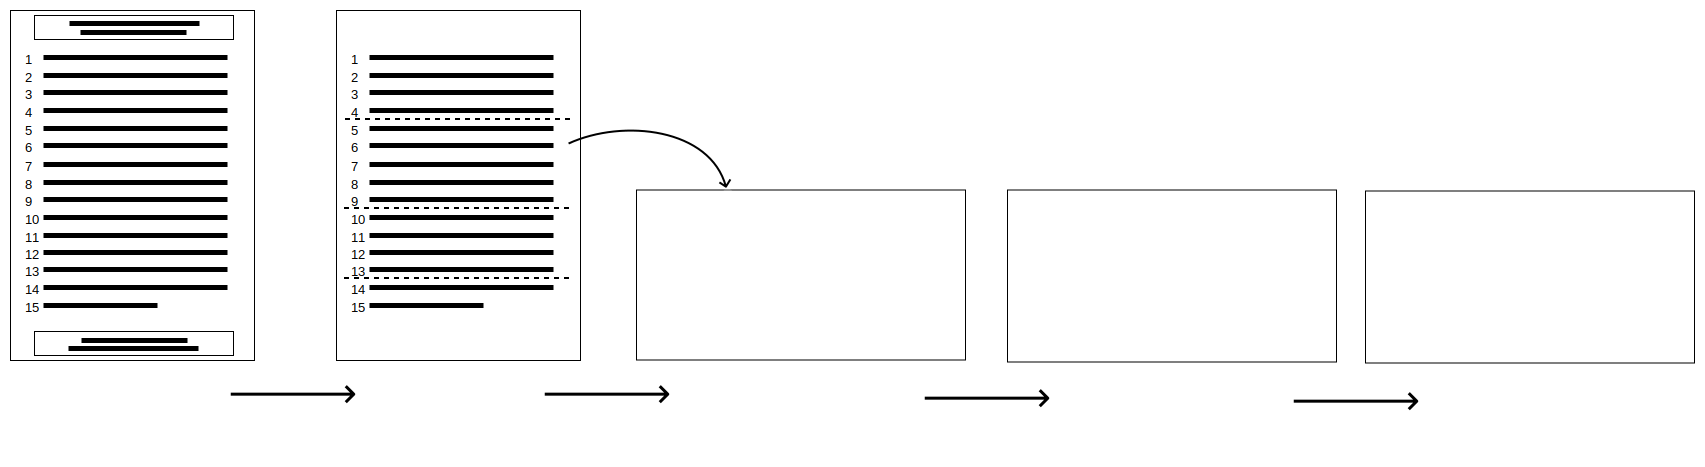
\includegraphics[trim={ 0 180 0 180 },clip,page=1,width=\textwidth]{conteudo/capitulos/figs/pre-process.pdf}

	\caption{Etapa de pré-processamento de um documento que inclui da remoção de elementos menos significativos e a identificação de sentenças}
	\label{fig:preprocessamento-segmentacao}
	\end{figure}
\end{center}



\begin{enumerate}

%  Cabeçalhos e rodapés
\item Remoção de cabeçalhos: as atas contém trechos que podem ser considerados pouco informativos e descartados durante o pré-processamento, como cabeçalhos e rodapés que se misturam aos tópicos tratados na reunião, podendo ser inseridos no meio de um tópico prejudicando tanto os algoritmos de MT e RI, quanto a leitura do texto pelo usuário. Um cabeçalho é a porção de texto que inicia cada página do documento e, de forma semelhante, um rodapé e a porção que as encerra. Detecta-se os cabeçalhos e os rodapés sempre que há uma repetição das primeiras e últimas palavras do documento.


%  Identificação de sentenças
\item Identificação sentenças: Nesse trabalho considera-se as sentenças as menor unidade de informação a ser processada pelos algoritmos de segmentação, por tanto, devem ser identificadas. Ao considerar intuitivamente que uma sentença seja uma sequência de palavras entre sinais de pontuação como ``.'', ``!'' e ``?'', alguns erros poderiam ocorrer quando esses tiverem outra função dentro do texto como em abreviações\footnote{As abreviações são identificadas por meio de uma lista com 234 abreviações conhecidas.}, endereços de internet e datas. Outro problema seriam frases curtas com poucas palavras e que não expressam um conceito completo, mas parte dele. Devido ao estilo de pontuação desses documentos, como encerrar sentenças usando um \textit{``;''} e inserção de linhas extras, foram usadas as regras especiais para identificação de finais de sentença. No Algoritmo~\ref{alg:identificacaofinaisdesent} é mostrado como cada \textit{token} é identificado e marcado com final de sentença.%, esse processo é melhor descrito na Subseção~\ref{subsec:indentificacaosentencas}. % Os detalhes sobre essas regras estão disponíveis para consulta em \urlsoftwares.



\begin{algorithm}
	\SetKwInOut{Input}{Entrada}
	\SetKwInOut{Output}{Saída}
	\SetKwBlock{Inicio}{início}{fim}
	\SetKwFor{ParaTodo}{para todo}{}{fim para todo}
	\SetKwIF{Se}{SenaoSe}{Senao}{}{}{senao se}{senao}{fim se}
	\SetKwFor{Para}{}{}{}
%	\SetKwAlgorithm{Algorithm}{Algoritmo}{}

	
	\Input{Texto}
	\Output{Texto com identificações de finais de sentença}
	
	\ParaTodo {token, marcá-lo como final de sentença se:} {	

	Terminar com um \texttt{!}\\
	Terminar com um \texttt{.} e não for uma abreviação\\
	Terminar em \texttt{.?;} e:
		\Para{}{
			For seguido de uma quebra de parágrafo ou tabulação\\
			O próximo \textit{token} iniciar com  \texttt{(\{["'}\\
			O próximo \textit{token} iniciar com letra maiúscula\\
			O penúltimo caracter  for \texttt{)\}]"'}\\
		}
	}
	
	\caption{Identificação de finais de sentença.}
	\label{alg:identificacaofinaisdesent}
\end{algorithm}


% TODO: "Pra que fazer isso?"


%  Remoção de termos
\item Redução de elementos menos significativos: Removeu-se do textos os termos que não contribuem para a etapa de segmentação, 
	as quais são chamadas de \textit{stop words}. Palavras como artigos, preposições, pronomes, verbos de estado\footnote{Apresentam uma situação inativa, onde o verbo não expressa uma alteração, mas apenas uma propriedade ou condição dos envolvidos.}. Trata-se também como \textit{stop words} as palavras de uso muito frequente dentro de um determinado domínio as quais não são capazes de discriminar textos, portanto também não devem fazer parte dos atributos~\cite{Rezende2003}. Para removê-las, as letras foram convertidas em caixa baixa e usou-se uma lista de 438 palavras para identificá-las. Além disso, eliminou-se a acentuação, sinais de pontuação, numerais e todos os termos menores que três caracteres.

%  Stemming
\item \textit{Stemming}: extraiu-se o radical de cada palavra. Para isso, aplicou-se o algoritmo \textit{Orengo} %\footnote{http://www.inf.ufrgs.br/~viviane/rslp/} 
	para remoção de sufixos~\cite{Alvares2005}.

\end{enumerate}
	



% ==================== Segmentação ===================== %


\subsection{Segmentação}

Como já mencionado, uma ata registra a sucessão de assuntos discutidos em uma reunião, porém apresenta-se com poucas quebras de parágrafo e sem marcações de estrutura, como capítulos, seções ou quaisquer indicações sobre o assunto do texto. Portanto, faz-se necessário descobrir quando há uma mudança de assunto no texto da ata. Para essa tarefa, as técnicas de segmentação de texto recebem uma lista de sentenças, da qual considera cada ponto entre duas sentenças como candidato a limite, ou seja, um ponto onde há transição entre assuntos~\cite{Bokaei2015, Bokaei2016, Misra2009, Sakahara2014}.

As técnicas de segmentação aboradas na Subseção~\ref{sec:segmentacao} divdiem o texto de cada ata em trechos que contêm um assunto relativamente independente, aqui chamdaos de sub-documentos. Esses sub-documentos serão processados por um extrator de tópicos que irá extrair descritores e agrupalos por tópicos.







% ==================== O Corpus ===================== %


\subsection{O Corpus}

% Colocar um trecho de uma ata??

% ->------> Seleção das atas
Selecionou-se um conjunto de atas reais coletadas do Departamento de Computação da UFSCar campus Sorocaba. Analisou-se as atas públicas das reuniões do Conselho de Pós-Graduação e Conselho de Graduação desse departamento das quais foram selecionadas seis atas de cada conselho, sendo cinco referentes a reuniões ordinária e uma reunião extraordinária, totalizando doze documentos. Esses documentos foram escolhidos de forma que o conjunto final contenha atas com tamanhos diferentes (entre 1 e 4 páginas), e maior diversidade de conteúdo.
 % contém tabelas e listas



















\chapter{Avaliação dos Segmentadores}\label{cap-segmentadores}




Nesse capítulo é apresentada uma análise dos algoritmos de segmentação textual com objetivo de iniciar uma discussão sobre a potencialidade das técnicas a serem utilizadas em um \textit{corpus} constituído de atas de reuniões conforme já mencionado na Seção~\ref{subsec:composicaocorpus}. 
Os algoritmos \textit{TextTiling} e \textit{C99} são analisados devido a sua abordagem linguística baseada em coesão léxica e por estarem entre os primeiros trabalhos nessa área e serem frequentemente referenciados até hoje~\cite{AlemiG15}. 
%	
Selecionou-se também os algoritmos \textit{BayesSeg} e \textit{TextSeg} por trazerem abordagens probabilísticas e o \textit{MinCutSeg} o qual é baseado em particionamento de grafos.
% 
Além disso, incluiu-se também um algoritmo que simplesmente atribui um segmento a cada sentença chamado aqui de \textit{PseudoSeg} para fins de comparação com as técnicas anteriores.

% ----- Segmnetação de Referência -----
A avaliação objetiva de um segmentador automático de textos exige uma referência, isto é, um conjunto de textos com os limites entre os segmentos conhecidos. Essa referência, deve ser confiável, sendo uma segmentação legítima que é capaz de dividir o texto em porções relativamente independentes, ou seja, uma segmentação ideal.

Aqui será detalhada uma avaliação objetiva em que os resultados dos algoritmos foram avaliados por sua similaridade com uma segmentação de referência construída com base na metodologia de anotações em sub-tópicos proposta em~\cite{Hovy2010}. Em seguida escolheu-se o modelo que apresenta melhores resultados para ser utilizado em conjunto com técnicas de extração de tópicos em um experimento onde se avaliou a performance de ambas as técnicas junto a profissionais com afinidade com atas de reunião que forneceram suas percepções em relação aos resultados do segmentador empregado nesse trabalho. Os dados obtidos dos experimentos serviram de base para as análises dos algoritmos e de sua aplicação no contexto das atas de reuniões. 
Optou-se por criar um \textit{corpus} de atas de reunião anotadas a fim de produzir-se uma segmentação de referência para avaliações dos algoritmos, bem como sua publicação e utilização em outros trabalhos voltados a esse domínio. O processo de anotação e criação da segmentação de referência está detalhada nas próximas seções.  

Nas próximas seções serão avaliados os segmentadores abordados nesse trabalho. Inicialmente é descrita a preparação do \textit{copus} e em seguida são detalhada as configurações utilizadas pelos algoritmos, bem como os critérios considerados para avaliá-los. Por fim, os resultados são apresentados e discutidos.



% =========== Avaliação dos Segmentadores ============ %
% \subsection{Avaliação dos Segmentadores}

\section{Preparação de um corpus de referência}




% ----- Anotação -----
Como já mencionado, a preparação desso corpus anotado teve como guia a metodologia introduzida em~\cite{Hovy2010} a qual indica sete passos para obter um corpus anotado. Essa metodologia está descrita na da Seção~\ref{sec:anotacoes} e explicada em~\cite{Cardoso2017}. 



% -- 1 - Escolha do Corpus
% O autor da metodologia indica que 
% Inicialmente, escolheu-se como \textit{corpus} a ser anotado	
O processo de anotação iniciou-se com a seleção de 12 atas de reuniões do departamento de computação da Universidade Federal de São Carlos campus Sorocaba, as quais são disponibilizadas publicamente\footnote{Acessível em  http://www.ppgccs.net/?page_id=1150}. Foram coletadas 6 atas de reuniões da Comissão do Curso de Pós-Graduação em Ciência da Computação e 6 atas de reuniões do Conselho do Curso de Bacharelado em Ciência da Computação, sendo 5 referentes a reuniões ordinárias e 1 extraordinária de cada setor.

% -- 2 - Escolha da teoria a ser explicada
O trabalho de anotação, visa identificar como usuários entendem as transições de assunto no documento, visto a ausência de marcações e meta informações no texto. Além disso, as anotações desse trabalho devem registrar o entendimento dos usuários em relação aos assuntos de cada segmento identificado e classificá-los quanto ao tipo de menção dada ao assunto. Maiores detalhes sobre a segmentação e rotulação manual serão fornecidos mais adiante nessa seção.
% do assunto como decisão, informe, irrelevante
% Com essas anotações pretende-se explicar como os usuários entendem a segmentação e lhes atribui tópicos.


% -- 3 - Selecionar e treinar os anotadores 
% -- 5 - Modelar uma interface para anotação
Após a delimitação do fenômeno a ser explicado e escolha do \textit{corpus} apropriado, selecionou-se um grupo de anotadores para analisar e coletar dados referentes a cada ata. O grupo de anotadores foi formado por profissionais com alguma afinidade com atas de reunião, como profissionais administrativos, professores e coordenadores de curso. 
A fim de facilitar o trabalho de anotação e diminuir eventuais erros, optou-se por desenvolver um \textit{software}\footnote{Códigos fontes disponíveis em: \url{https://github.com/ovidio-francisco/UFSCar/tree/master/codes/TextSegmentationTool} } como ferramenta para a coleta dos dados, conforme sugerido em~\cite{Hovy2010}. Essa ferramenta foi modelada para permitir aos anotadores visualizar os documentos e indicar livremente as divisões entre segmentos, bem como rotulá-los. 

Nesse processo, rotulou-se o assunto tratado no seguimento em 3 passos:
(1) classificação quanto ao tipo de comunicação, onde se especificou uma entre as opções 
\textit{``decisão``},
\textit{``informe''},
\textit{``irrelevante''} e 
\textit{``outro''} sendo que para essa última, o anotador poderia especificar livremente a classe.
(2) classificação quanto ao ao contexto onde se gerou o assunto, onde as classes, 
\textit{``discussão''},
\textit{``orientação''},
\textit{``solicitação''} e 
\textit{``outro''} podendo o anotador indicá-las simultaneamente.
(3) descrição do assunto, onde o anotador apontou até 5 palavras contidas no texto para representar o teor do segmento.
Na Figura~\ref{fig:interfaceanotacoes} é mostrada a interface da ferramenta utilizada para as anotações.

De acordo com a literatura a respeito de anotações em sub-tópicos, é recomendável fornecer treinamento aos participantes. Nesse trabalho os anotadores receberam apenas informações básicas sobre o objetivo da pesquisa e instruções de como operar o \textit{software} por meio de um vídeo\footnote{Acessível em }, deixando o entendimento sobre a segmentação e rotulação a critério de cada anotador. Assim, nenhum critério foi estabelecido para o procedimento ficando os anotadores orientados apenas pela interface da ferramenta. 

  \begin{figure}[!h]
	  \centering
	  \includegraphics[width=1\textwidth]{conteudo/capitulos/figs/interface-anotacoes.png}
	  \caption{Interface da ferramenta utilizada para anotações onde o texto a ser segmentado é exibido no painel a esquerda e os controles para anotação estão disponíveis a direita.}
	  \label{fig:interfaceanotacoes}
  \end{figure}



% -- 4 - Especificar o procedimento de anotação
O procedimento de anotação deu-se remotamente. Os anotadores receberam por e-mail o acesso ao \textit{software} e individualmente realizaram as anotações. A tarefa de segmentar e rotular manualmente demandou em torno de 4 a 6 horas de atenção dos anotadores. Em razão desse esforço, o \textit{software} permitiu que a tarefa fosse pausada e reiniciada sempre que houvesse necessidade, sem prejuízos ao trabalho.



% Os arquivos gerados foram tratados para que os segmentos sempre terminem em uma sentença reconhecida pelo algoritmo, uma vez que as sentenças são a unidade mínima de informação nesse trabalho.
O \textit{corpus} anotado deve ser constituído a partir dos textos originais e da resultante das percepções dos anotadores a certa do fenômeno a ser explicado. Assim, o texto de cada uma das 12 atas selecionadas será acrescido de informações geradas a partir dos dados coletados. Após o processo de anotação, a segmentação de referência foi criada utilizando o critério de maior concordância, como já relatado em outros trabalhos~\cite{Hearst1997, Cardoso2017, Kazantseva2012, Passonneau1997, Galley2003}. Assim, considerou-se que ocorre um limite entre segmentos quando a maioria dos anotadores (metade mais um) concordou que a mesma sentença é um final de segmento. 

Na Figura~\ref{fig:concordanciasegref} é mostrado um exemplo de criação de uma segmentação de referência por meio da concordância entre anotadores. As primeiras linhas representam segmentações fornecidas por anotadores e a última linha representa a segmentação resultante da concordância entre a maioria dos segmentadores e portanto mais confiável. 

  \begin{center}
	\begin{figure}[h!]

	\includegraphics[trim={ 95 255 75 140 },clip,page=1,width=\textwidth]{conteudo/capitulos/figs/segmentacao-referencia.pdf}

	\caption{Exemplo uma segmentação de referência criada a partir da concordância entre segmentações manuais.}
	\label{fig:concordanciasegref}
	\end{figure}
\end{center}







% ----------------- Exemplo Segmentação de Referência ----------------------

Na Tabela~\ref{tab:segmentacaoreferencia} é mostrado um exemplo em que 6 dos 9 anotadores concordaram a respeito de um segmento. A tabela mostra quatro segmentos extraídos da segmentação de referência onde cada linha contém um segmento e os índices a esquerda indicam uma sentença. Junto à cada segmento é mostrada  a classe e descritores rotulados por um dos anotadores. Vale ressaltar que esses rótulos não foram utilizados no processo de segmentação e não têm nenhuma influência sobre a segmentação de referência. %Nesse trabalho, essas anotações são utilizadas na avaliação dos extratores de tópicos. --> não é

\begin{table}[!h]
	\centering 
\footnotesize
% \scriptsize
	\begin{tabular}{|p{0.2cm}p{14,5cm}|} \hline


$^{[7]}$&
(II) Encerrada a etapa de inscrição para o processo seletivo como aluno regular para o segundo semestre de 2015: foram quarenta e nove inscrições on-line e dezoito candidatos entregaram a documentação; 
\textit{<informe>} \textit{<processo;seletivo>}
\\ \hline


$^{[8]}$ &
(III) O Prof. Dr. AAA informou que a Pró-Reitora comunicou a oferta de mais uma bolsa pela cota da Pró-Reitoria, mas não havia aluno disponível para alocação da bolsa.\\
$^{[9]}$ &
(III) O Prof. Dr. AAA informou que a Pró-Reitora comunicou a oferta de mais uma bolsa pela cota da Pró-Reitoria, mas não havia aluno disponível para alocação da bolsa.\\
$^{[10]}$ &
O Prof. Dr. BBB informou que havia uma aluna interessada, mas não informada durante o processo de elaboração do ranking no início do semestre.\\
$^{[11]}$ &
Ficou decidido enviar e-mail aos docentes solicitando que comuniquem permanentemente interesse de alunos em bolsa pra atualização do ranking;
\textit{<informe>} \textit{<solicitação;bolsa;cota;ranking;alunos>}
\\ \hline


$^{[12]}$ &
(IV) Com a mudança do Prof. Dr. DDD para o campus de São Carlos, o Prof. Dr. BBB assume o posto de suplente da linha Teoria Aplicada à Computação na CPG;
\textit{<informe>} \textit{<mudança;suplente;teoria;aplicada;computação>}
\\ \hline

$^{[13]}$ &
	Comunicação dos membros: Não houve;
	\textit{<irrelevante>} 
\\ \hline



% $^{[14]}$ &
% Ordem do Dia: (I) Foram apresentadas regras para participação de membro externo em banca de defesa do mestrado.\\
% $^{[15]}$ &
% O Prof. Dr. Alexandre Alvaro comentou que está sendo pago aos participantes externos das bancas a diária pelo PROAP e o pró-labore pelo DComp, além do programa fornecer o transporte, que onera a verba PROAP.\\
% $^{[16]}$ &
% O Prof. Dr. Tiago Agostinho de Almeida sugeriu o seguinte cálculo para pagamento: se o participante vier de uma Instituição com distância até 220 km será feito o cálculo de R\$ 1,00 multiplicado pela quilometragem.\\
% $^{[17]}$ &
% Caso a distância seja superior a 220 km, será calculada a distância multiplicada por R\$ 0,60. O menor valor entre o custo do transporte e o pagamento de verba e pró-labore será utilizado para custear a vinda do participante;
% \\ \hline



% $^{[18]}$ &
% (II) Foi discutida a forma de convalidação de disciplinas cursadas como aluno regular anterior a três anos do reingresso do aluno.
% Foi decidido que fica a cargo da CPG decidir sobre as disciplinas que serão aproveitadas quando do reingresso do aluno;
% \\ \hline



% $^{[13]}$ &

	\end{tabular}
	\caption{Exemplo de segmentação de referência com rotulação de um anotador}
	\label{tab:segmentacaoreferencia}
\end{table}









  




% -- 6 - Escolher e aplicar medidas de avaliação
Para mensurar a concordância entre anotadores, a medida \textit{kappa (k)}~\cite{Carletta1996} é frequentemente utilizada~\cite{Gruenstein2007, Cardoso2017, Hearst1997}. Ela mostra como os anotadores compreendem os textos analisados e o nível de confiabilidade da segmentação de referência. Essa medida retorna um valor no intervalo de 0 até 1, onde 1 significa uma concordância perfeita e 0 que não houve concordância. 
% As medidas de similaridade entre segmentações também podem ser utilizadas para avaliar a qualidade da segmentação de referência. 
As medidas \textit{WindowDiff} e $P_k$ informam a probabilidade de duas sentenças escolhidas aleatoriamente estarem no mesmo segmento. Elas refletem a similaridade entre duas segmentações, assim também podem ser utilizadas para avaliar a concordância entre os anotadores. As formulações dessas medidas são abordadas em mais detalhes na Seção~\ref{subsec:medidas-segmentacao}.
Nesse trabalho, para cada segmentação fornecida por cada anotador calcula-se as medidas \textit{WindowDiff}, $P_k$ e \textit{Kappa}.
A Tabela~\ref{tab:ataseanotacoes} contém, para cada ata, a quantidade de sentenças e a quantidade de segmentos identificadas pelos participantes e as médias de \textit{WindowDiff}, $P_k$ e \textit{Kappa}. Uma vez que P$_k$ e \textit{WindowDiff}, são medidas de dissimilaridade, são reportados os seus complementos.
% Uma vez que P$_k$ e WD, indicam melhores valores próximos a 0 e 1 como dissimilarid 

\begin{table}[!h]
	\centering
	\begin{tabular}{|l|c|c|c|c|c|c|c|c|c|c|c|c|c|} \hline
		\textbf{Ata} & \textbf{Sent.}  & 
		\textbf{A1}  & 
		\textbf{A2}  & 
		\textbf{A3}  & 
		\textbf{A4}  & 
		\textbf{A5}  & 
		\textbf{A6}  & 
		\textbf{A7}  & 
		\textbf{A8}  & 
		\textbf{A9} 
		% &
		% \textbf{k}  &
		% \textbf{P$_k$}  &
		% \textbf{WD}  
		\\	\hline

% &  0.344 & 0.593 & 0.475 
% &  0.377 & 0.572 & 0.509 
% &  0.384 & 0.603 & 0.524 
% &  0.447 & 0.652 & 0.540 
% &  0.315 & 0.595 & 0.364 
% &  0.397 & 0.605 & 0.576 
% &  0.374 & 0.658 & 0.506 
% &  0.378 & 0.611 & 0.471 
% &  0.428 & 0.591 & 0.478 
% &  0.309 & 0.598 & 0.233 
% &  0.348 & 0.645 & 0.412 
% &  0.278 & 0.577 & 0.102 

% 		              A1   A2   A3  A4    A5   A6   A7   A8   A9   
		Ata 1  & 25 & 7  & 4  & 11 & 6  & 16 & 8  & 8  & 15 & 16 \\ \hline 
		Ata 2  & 17 & 4  & 4  & 8  & 6  & 11 & 6  & 6  & 15 & 14 \\ \hline 
		Ata 3  & 26 & 6  & 6  & 8  & 4  & 15 & 9  & 10 & 18 & 14 \\ \hline 
		Ata 4  & 26 & 5  & 5  & 10 & 6  & 14 & 17 & 7  & 11 & 12 \\ \hline 
		Ata 5  & 33 & 4  & 4  & 6  & 5  & 17 & 22 & 9  & 18 & 16 \\ \hline 
		Ata 6  & 11 & 3  & 4  & 6  & 4  & 9  & 9  & 4  & 7  &  5 \\ \hline 
		Ata 7  & 20 & 3  & 7  & 5  & 4  & 11 & 14 & 5  & 5  &  4 \\ \hline 
		Ata 8  & 35 & 4  & 8  & 3  & 8  & 12 & 17 & 5  & 11 &  9 \\ \hline 
		Ata 9  & 24 & 3  & 5  & 3  & 6  & 11 & 11 & 3  & 9  &  9 \\ \hline 
		Ata 10 & 50 & 4  & 5  & 4  & 7  & 31 & 29 & 5  & 9  &  8 \\ \hline 
		Ata 11 & 43 & 4  & 7  & 5  & 7  & 29 & 19 & 5  & 9  & 12 \\ \hline 
		Ata 12 & 56 & 3  & 10 & 4  & 16 & 33 & 25 & 4  & 13 & 11 \\ \hline 
		\textbf{Total} &
		\textbf{366} & 
		\textbf{50}&  
		\textbf{69} & 
		\textbf{73}&  
		\textbf{79}&  
		\textbf{20}9 & 
		\textbf{186}&  
		\textbf{71}&  
		\textbf{140}&  
		\textbf{130} 
		% & 
		% \textbf{0.364} & 
		% \textbf{0.608} & 
		% \textbf{0.432} 
		\\ \hline 

	\end{tabular}
	% \caption{Quantidade de sentenças e segmentos de referência por ata.}
	\caption{Descrição dos resultados obtidos com anotadores. Na segunda coluna Sent., é mostrada a quantidade de sentenças de cada ata. Nas colunas A1-A9 é mostrado as quantidades de segmentos informados pelos anotadores. As colunas K, P$_k$ e WD indicam respectivamente as médias de \textit{Kappa}, $P_k$ e \textit{WindowDiff}.} 

	\label{tab:ataseanotacoes}
\end{table}


Os valores de \textit{Kappa} reforça que a tarefa de segmentação é bastante subjetiva e indicam que, nesse contexto, a segmentação de referência resultante é pouco confiável, visto os baixos valores de concordância entre os anotadores. 
Embora~\cite{Carletta1996} afirme que valores de $k~>~0,8$ indicam que os dados são confiáveis, visto a subjetividade da tarefa de segmentação textual, medidas menores podem ser aceitáveis, como reportado em~\cite{Hearst1997} que alcançou $k~=~0,64$ e~\cite{Cardoso2017}, $k~=~0,56$. Além dos baixos valores para as medidas nota-se também que o anotadores divergem na quantidade de segmentos, o que sugere que diferentes anotadores tem percepções distintas quanto a granularidade de assuntos, ou seja, trechos com pequenas mudanças de assunto são entendidas como segmentos diferentes por alguns anotadores, enquanto outros entendem como pertencentes ao mesmo assunto.


% - maior granularidade é preferivel, pois evita omição de informação.



% -- 7 - disponibilizar e manter o produto
Após a coleta dos dados das anotações e construção da segmentação de referência, o \textit{corpus} anotado serviu de como base para avaliação dos segmentadores bem como aspectos da configuração e avaliação dos extratores de tópicos no Capítulo~\ref{cap-extratores}. Além da utilidade prestada a esse trabalho, o produto do resultante do processo de anotação está disponibilizado para outros trabalhos voltados a esse domínio.



\begin{table}[!h]
	\centering
 \begin{tabular}{|l|c|c|c|c|}

\hline
Referência  & \#Seg & \textit{Kappa}       & $P_k$                &  \textit{WinDiff}\\ \hline
Ref. 01     & 15    & 0.344  $\sigma$0.190 & 0.433  $\sigma$0.170 & 0.631  $\sigma$0.409 \\ \hline
Ref. 02     & 13    & 0.266  $\sigma$0.246 & 0.439  $\sigma$0.190 & 0.565  $\sigma$0.379 \\ \hline
Ref. 03     & 15    & 0.328  $\sigma$0.183 & 0.442  $\sigma$0.165 & 0.590  $\sigma$0.353 \\ \hline
Ref. 04     & 15    & 0.364  $\sigma$0.241 & 0.364  $\sigma$0.161 & 0.562  $\sigma$0.377 \\ \hline
Ref. 05     & 19    & 0.315  $\sigma$0.217 & 0.458  $\sigma$0.223 & 0.889  $\sigma$0.640 \\ \hline
Ref. 06     & 9     & 0.314  $\sigma$0.218 & 0.404  $\sigma$0.163 & 0.463  $\sigma$0.266 \\ \hline
Ref. 07     & 8     & 0.235  $\sigma$0.208 & 0.343  $\sigma$0.192 & 0.507  $\sigma$0.401 \\ \hline
Ref. 08     & 12    & 0.211  $\sigma$0.225 & 0.421  $\sigma$0.186 & 0.629  $\sigma$0.479 \\ \hline
Ref. 09     & 12    & 0.234  $\sigma$0.258 & 0.472  $\sigma$0.203 & 0.660  $\sigma$0.427 \\ \hline
Ref. 10     & 13    & 0.170  $\sigma$0.206 & 0.428  $\sigma$0.227 & 0.937  $\sigma$1.050 \\ \hline
Ref. 11     & 12    & 0.209  $\sigma$0.236 & 0.368  $\sigma$0.203 & 0.704  $\sigma$0.654 \\ \hline
Ref. 12     & 21    & 0.222  $\sigma$0.195 & 0.452  $\sigma$0.200 & 1.113  $\sigma$1.202 \\ \hline
 
\end{tabular}
\caption{Detalhes da Segmentação de Referência.}
\label{tab:detalhesSegRef}
\end{table}












\section{Configuração experimental}
\label{subsec:configuracaoexperimental}

  

% -> Parâmetros do TT
O \textit{TextTiling} permite ajustarmos dois parâmetros, sendo o tamanho da janela e o passo. Por meio de testes empíricos escolheu-se os valores os valores 20, 40 e 60 para o tamanho da janela e 3, 6, 9 e 12 para o passo, gerando ao final 20 configurações.
%

% -> Parâmetros do C99
O \textit{C99} permite o ajuste de três parâmetros, sendo, o primeiro a quantidade segmentos desejados, uma vez que não se conhece o número ideal de segmentos, configurou-se a quantidade de segmentos com base em uma proporção dos candidatos a limite. Para isso atribuiu-se os valores {0,2; 0,4; 0,6; 0,8}. Para o segundo parâmetro, o tamanho do quadro utilizado para gerar a matriz de ranking, atribuiu-se os valores 9 e 11, sendo 11 o valor padrão da apresentado pelo autor. O algoritmo permite ainda indicar se as sentenças serão representadas por vetores contendo a frequência ou o peso de cada termo. Ambas as representações foram utilizadas. Considerando todos os parâmetros, foram geradas 16 configurações para o algoritmo \textit{C99}.

Os algoritmos tradicionais baseados em coesão léxica como o \textit{TextTiling} e \textit{C99} são fortemente afetados pela distribuição das palavras no texto, pois a maioria das medidas de similaridade baseiam-se na frequência das palavras. Para esses, a remoção de termos menos significativos na etapa de pré-processamento pode influenciar o desempenho. Para outras abordagens como \textit{MinCutSeg} e \textit{BayesSeg} usou-se as configurações fornecidas por~\cite{Eis2008}, onde essas técnicas foram utilizadas como \textit{base line}. Para \textit{TextSeg} não requer configuração de parâmetros.
Há ainda outras estratégias passíveis de aplicação, como a utilização de fontes externas, por exemplo \textit{thesaurus} e palavras pista, como discutido em \cite{Naili2016, Gutierrez2016, Ferret2009}. Nesse trabalho, essas estratégias não são utilizadas para manter uma abordagem não supervisionada e independente de domínio. 
Inicialmente, calculou-se as medidas configurando cada algoritmo
% conforme mostrado na Subseção~\ref{subsec:configuracaoexperimental} e, 
a fim de conhecer o impacto do pré-processamento nos algoritmos \textit{TextTiling} e \textit{C99}. Esses foram testados em duas etapas: com o texto integral, e com o texto pré-processado em que elementos menos significativos foram removidos, conforme mencionado na Seção~\ref{sec:modulo-preparacao}.  

\section{Critérios de avaliação}

% -> Definição do que é um bom algoritmo de segmentação
Para fins de avaliação desse trabalho, um bom método de segmentação é aquele cujo resultado melhor se aproxima da segmentação de referência, sem a obrigatoriedade de estar perfeitamente alinhado com tal. Ou seja, visto o contexto das atas de reunião, e a subjetividade da tarefa, não é necessário que os limites entre os segmentos (real e hipótese) sejam idênticos, mas que se assemelhem em localização e quantidade.

As segmentações obtidas com os algoritmos foram comparadas com a segmentação de referência obtida e calculou-se as medidas mais aplicadas à segmentação textual, $P_k$ e \textit{WindowDiff}. Além dessas, computou-se também as medidas tradicionais acurácia e $F^1$ para analises que considerando a exatidão desses técnicas.
% comparação com outros trabalhos que as utilizam.

O teste de Friedman foi utilizado para gerar um ranking das melhores configurações para cada medida calculada. Com isso, foi possível descobrir quais valores otimizam um algoritmo para cada medida, considerando seus parâmetros e a influência do pré-processamento. Como já mencionado, os algoritmos \textit{MinCutSeg} e \textit{BayesSeg} aplicou-se a etapa de pré-processamento e foram testados com as configurações apresentadas por~\cite{Eis2008}. 



\section{Resultados}

Obteve-se, por meio dos testes apresentados, as melhores configurações para as principais medidas de avaliação de segmentadores. Com essas configurações calculou-se a média de cada medida considerando o conjunto de documentos. Os algoritmos foram executados com as configurações apresentadas e discutidos mais adiante nessa seção.

A seguir são apresentados os resultados obtidos com os algoritmos baseados em coesão léxica (\textit{TextTiling} e \textit{C99}, considerando seus principais parâmetros e a aplicação do pré-processamento. Em seguida, são apresentados os resultados da avaliação geral de todos os algoritmos abordados nesse trabalho.

Na Tabela~\ref{tab:resultadosTT} são apresentadas, as médias obtidas com o \textit{TextTiling} bem como as configurações utilizadas, onde \textbf{J} é o tamanho da janela e \textbf{P} é o passo.



	



\begin{table}[!h]
\tiny \center
\textbf{TextTiling} \\ 
	\begin{tabular}{|c|c||c|c|c|c|c||c|c|c|c|c|}
\hline 
\multirow{2}{*}{Step} & \multirow{2}{*}{Win Size}
  & \multicolumn{5}{c||}{Com texto integral} & \multicolumn{5}{c|}{Com texto pré-processado}\\\cline{3-12} 
&& $WinDiff$ & $P_k$ & Acurácia & $F^1$ & \#Segs &  $WinDiff$ & $P_k$ & Acurácia & $F^1$ & \#Segs\\ \hline 
 \multirow{6}{*}{20} 
  & 30 & 0.513 & 0.490 & 0.538 & 0.334  & 8.500                 & 0,461 & 0,444 & 0,581 & \cellcolor{gray!20} \textbf{0,411} & 8,833  \\ \cline{2-12} 
  & 35 & 0.509 & 0.492 & 0.540 & 0.350  & 8.583                 & 0,462 & 0,443 & 0,582 & 0,401 & 8,750  \\  \cline{2-12}
  & 40 & 0.517 & 0.495 & 0.532 & 0.342  & 8.583                 & 0,485 & 0,466 & 0,562 & 0,378 & 8,250  \\  \cline{2-12}
  & 45 & 0.496 & 0.477 & 0.555 & 0.347  & 7.667                 & 0,480 & 0,458 & 0,572 & 0,369 & 8,250  \\  \cline{2-12}
  & 50 & 0.481 & 0.465 & 0.569 & \cellcolor{gray!20} \textbf{0.390} & 8.750  & 0,523 & 0,503 & 0,528 & 0,327 & 8,417  \\  \cline{2-12}
  & 55 & 0.512 & 0.493 & 0.542 & 0.337  & 8.250  & 0,491 & 0,474 & 0,549 & 0,331 & 8,250  \\ \hline      
 \multirow{6}{*}{30} 
  & 30 & 0.511 & 0.494 & 0.538 & 0.284  & 6.667                & 0,509 & 0,488 & 0,536 & 0,286 & 6,917  \\ \cline{2-12}    
  & 35 & 0.517 & 0.500 & 0.536 & 0.285  & 6.583                & 0,500 & 0,479 & 0,551 & 0,318 & 7,167  \\ \cline{2-12}         
  & 40 & 0.512 & 0.491 & 0.543 & 0.299  & 6.750                & 0,468 & 0,451 & 0,576 & 0,348 & 6,750  \\ \cline{2-12} 
  & 45 & 0.502 & 0.483 & 0.555 & 0.320  & 6.917                & \cellcolor{gray!20} \textbf{0,450} & \cellcolor{gray!20} \textbf{0,435} & \cellcolor{gray!20} \textbf{0,596} & 0,373 & 6,417  \\  \cline{2-12} 
  & 50 & 0.510 & 0.493 & 0.539 & 0.313  & 7.333                & 0,493 & 0,478 & 0,543 & 0,307 & 6,417  \\ \cline{2-12}                
  & 55 & 0.498 & 0.480 & 0.543 & 0.328  & 7.250                & 0,481 & 0,463 & 0,558 & 0,346 & 7,083  \\ \hline     
 \multirow{6}{*}{40} 
  & 30 & 0.493 & 0.477 & 0.555 & 0.248  & 4.917                & 0,475 & 0,460 & 0,566 & 0,306 & 5,833  \\ \cline{2-12} 
  & 35 & 0.482 & 0.465 & 0.558 & 0.267  & 5.417                & 0,501 & 0,482 & 0,542 & 0,268 & 6,083  \\ \cline{2-12} 
  & 40 & 0.476 & 0.459 & 0.565 & 0.275  & 5.500                & 0,499 & 0,478 & 0,548 & 0,293 & 6,083  \\ \cline{2-12} 
  & 45 & 0.501 & 0.482 & 0.549 & 0.260  & 5.333                & 0,488 & 0,471 & 0,551 & 0,275 & 5,500  \\ \cline{2-12} 
  & 50 & 0.498 & 0.481 & 0.551 & 0.266  & 5.333                & 0,495 & 0,474 & 0,552 & 0,280 & 5,833  \\ \cline{2-12} 
  & 55 & 0.505 & 0.487 & 0.544 & 0.243  & 5.083                & 0,476 & 0,453 & 0,567 & 0,310 & 6,083  \\ \hline      
 \multirow{6}{*}{50} 
 & 30 & \cellcolor{gray!20} \textbf{0.474} & \cellcolor{gray!20} \textbf{0.455} & \cellcolor{gray!20} \textbf{0.579} & 0.295 & 4.917 & 0,492 & 0,473 & 0,557 & 0,274 & 5,167  \\ \cline{2-12}
  & 35 & 0.528 & 0.511 & 0.531 & 0.202  & 4.583                & 0,504 & 0,484 & 0,549 & 0,268 & 5,583  \\ \cline{2-12} 
  & 40 & 0.501 & 0.488 & 0.539 & 0.234  & 5.000                & 0,501 & 0,481 & 0,556 & 0,278 & 5,417  \\ \cline{2-12} 
  & 45 & 0.489 & 0.476 & 0.558 & 0.275  & 5.167                & 0,508 & 0,484 & 0,549 & 0,264 & 5,500  \\ \cline{2-12} 
  & 50 & 0.498 & 0.483 & 0.545 & 0.304  & 6.083                & 0,513 & 0,491 & 0,536 & 0,253 & 5,417  \\ \cline{2-12} 
  & 55 & 0.490 & 0.470 & 0.556 & 0.303  & 5.583                & 0,509 & 0,487 & 0,543 & 0,276 & 5,833  \\ \hline      
 \multirow{6}{*}{60}                           
  & 30 & 0.499 & 0.486 & 0.557 & 0.234  & 4.417                & 0,481 & 0,462 & 0,564 & 0,267 & 4,917  \\ \cline{2-12} 
  & 35 & 0.509 & 0.494 & 0.537 & 0.243  & 5.000                & 0,503 & 0,483 & 0,549 & 0,250 & 5,083  \\ \cline{2-12} 
  & 40 & 0.501 & 0.486 & 0.545 & 0.182  & 3.833                & 0,497 & 0,481 & 0,554 & 0,242 & 4,750  \\ \cline{2-12} 
  & 45 & 0.493 & 0.478 & 0.558 & 0.227  & 4.167                & 0,465 & 0,448 & 0,577 & 0,271 & 4,500  \\ \cline{2-12} 
  & 50 & 0.495 & 0.478 & 0.562 & 0.225  & 4.083                & 0,478 & 0,459 & 0,569 & 0,250 & 4,333  \\ \cline{2-12} 
  & 55 & 0.500 & 0.485 & 0.550 & 0.198  & 4.000                & 0,474 & 0,457 & 0,568 & 0,269 & 5,000  \\ \hline      

 \end{tabular}  
 \label{tab:resultadosTT}
\caption{Resultados do TextTiling considerando o pré-processamento.}
\end{table} 

























% \begin{table}[!h]
% \tiny \center
% \textbf{TextTiling} \\ 
	% \begin{tabular}{|c|c||c|c|c|c|c||c|c|c|c|c|}
% \hline 
% \multirow{2}{*}{Step} & \multirow{2}{*}{Win Size}
  % & \multicolumn{5}{c||}{Com texto pré-processado} & \multicolumn{5}{c|}{Com texto integral}\\\cline{3-12} 
% && $WinDiff$ & $P_k$ & Acurácia & $F^1$ & \#Segs &  $WinDiff$ & $P_k$ & Acurácia & $F^1$ & \#Segs\\ \hline 
 % \multirow{6}{*}{20} 

 % & 30                                   & 0,461 & 0,444 & 0,581 & \cellcolor{gray!20} \textbf{0,411} & 8,833                                                                                       & 0.513 & 0.490 & 0.538 & 0.334  & 8.500                                                                                           \\ \cline{2-12} 
 % & 35                                   & 0,462 & 0,443 & 0,582 & 0,401 & 8,750                                                                                                                    & 0.509 & 0.492 & 0.540 & 0.350  & 8.583                                                                                           \\  \cline{2-12}
 % & 40                                   & 0,485 & 0,466 & 0,562 & 0,378 & 8,250                                                                                                                    & 0.517 & 0.495 & 0.532 & 0.342  & 8.583                                                                                           \\  \cline{2-12}
 % & 45                                   & 0,480 & 0,458 & 0,572 & 0,369 & 8,250                                                                                                                    & 0.496 & 0.477 & 0.555 & 0.347  & 7.667                                                                                           \\  \cline{2-12}
 % & 50                                   & 0,523 & 0,503 & 0,528 & 0,327 & 8,417                                                                                                                    & 0.481 & 0.465 & 0.569 & \cellcolor{gray!20} \textbf{0.390} & 8.750                                                               \\  \cline{2-12}
 % & 55                                   & 0,491 & 0,474 & 0,549 & 0,331 & 8,250                                                                                                                    & 0.512 & 0.493 & 0.542 & 0.337  & 8.250                                                                                           \\ \hline      
 % \multirow{6}{*}{30}                                                                                                                                                                                                                                                                                                                                     
 % & 30                                   & 0,509 & 0,488 & 0,536 & 0,286 & 6,917                                                                                                                    & 0.511 & 0.494 & 0.538 & 0.284  & 6.667                                                                                            \\ \cline{2-12} 
 % & 35                                   & 0,500 & 0,479 & 0,551 & 0,318 & 7,167                                                                                                                    & 0.517 & 0.500 & 0.536 & 0.285  & 6.583                                                                                            \\ \cline{2-12} 
 % & 40                                   & 0,468 & 0,451 & 0,576 & 0,348 & 6,750                                                                                                                    & 0.512 & 0.491 & 0.543 & 0.299  & 6.750                                                                                            \\ \cline{2-12} 
 % & 45                                   & \cellcolor{gray!20} \textbf{0,450}  & \cellcolor{gray!20} \textbf{0,435} & \cellcolor{gray!20} \textbf{0,596} & 0,373 & 6,417                            & 0.502 & 0.483 & 0.555 & 0.320  & 6.917                                                                                            \\  \cline{2-12} 
 % & 50                                   & 0,493 & 0,478 & 0,543 & 0,307 & 6,417                                                                                                                    & 0.510 & 0.493 & 0.539 & 0.313  & 7.333                                                                                            \\ \cline{2-12}   
 % & 55                                   & 0,481 & 0,463 & 0,558 & 0,346 & 7,083                                                                                                                    & 0.498 & 0.480 & 0.543 & 0.328  & 7.250                                                                                            \\ \hline     
 % \multirow{6}{*}{40}                                                                                                                                                                                                                                                                                                                                       
 % & 30                                   & 0,475 & 0,460 & 0,566 & 0,306 & 5,833                                                                                                                    & 0.493 & 0.477 & 0.555 & 0.248  & 4.917                                                                                            \\ \cline{2-12} 
 % & 35                                   & 0,501 & 0,482 & 0,542 & 0,268 & 6,083                                                                                                                    & 0.482 & 0.465 & 0.558 & 0.267  & 5.417                                                                                            \\ \cline{2-12} 
 % & 40                                   & 0,499 & 0,478 & 0,548 & 0,293 & 6,083                                                                                                                    & 0.476 & 0.459 & 0.565 & 0.275  & 5.500                                                                                            \\ \cline{2-12} 
 % & 45                                   & 0,488 & 0,471 & 0,551 & 0,275 & 5,500                                                                                                                    & 0.501 & 0.482 & 0.549 & 0.260  & 5.333                                                                                             \\ \cline{2-12} 
 % & 50                                   & 0,495 & 0,474 & 0,552 & 0,280 & 5,833                                                                                                                    & 0.498 & 0.481 & 0.551 & 0.266  & 5.333                                                                                             \\ \cline{2-12} 
 % & 55                                   & 0,476 & 0,453 & 0,567 & 0,310 & 6,083                                                                                                                    & 0.505 & 0.487 & 0.544 & 0.243  & 5.083                                                                                             \\ \hline      
 % \multirow{6}{*}{50}                                                                                                                                                                                                                                                                                                                                  
 % & 30                                   & 0,492 & 0,473 & 0,557 & 0,274 & 5,167                                                                                                                    & \cellcolor{gray!20} \textbf{0.474} & \cellcolor{gray!20} \textbf{0.455} & \cellcolor{gray!20} \textbf{0.579} & 0.295 & 4.917      \\ \cline{2-12}
 % & 35                                   & 0,504 & 0,484 & 0,549 & 0,268 & 5,583                                                                                                                    & 0.528 & 0.511 & 0.531 & 0.202  & 4.583                                                                                            \\ \cline{2-12} 
 % & 40                                   & 0,501 & 0,481 & 0,556 & 0,278 & 5,417                                                                                                                    & 0.501 & 0.488 & 0.539 & 0.234  & 5.000                                                                                            \\ \cline{2-12} 
 % & 45                                   & 0,508 & 0,484 & 0,549 & 0,264 & 5,500                                                                                                                    & 0.489 & 0.476 & 0.558 & 0.275  & 5.167                                                                                            \\ \cline{2-12} 
 % & 50                                   & 0,513 & 0,491 & 0,536 & 0,253 & 5,417                                                                                                                    & 0.498 & 0.483 & 0.545 & 0.304  & 6.083                                                                                            \\ \cline{2-12} 
 % & 55                                   & 0,509 & 0,487 & 0,543 & 0,276 & 5,833                                                                                                                    & 0.490 & 0.470 & 0.556 & 0.303  & 5.583                                                                                            \\ \hline      
 % \multirow{6}{*}{60}                                                                                                                                                                                                                                                                                                                      
 % & 30                                   & 0,481 & 0,462 & 0,564 & 0,267 & 4,917                                                                                                                    & 0.499 & 0.486 & 0.557 & 0.234  & 4.417                                                                                            \\ \cline{2-12} 
 % & 35                                   & 0,503 & 0,483 & 0,549 & 0,250 & 5,083                                                                                                                    & 0.509 & 0.494 & 0.537 & 0.243  & 5.000                                                                                            \\ \cline{2-12} 
 % & 40                                   & 0,497 & 0,481 & 0,554 & 0,242 & 4,750                                                                                                                    & 0.501 & 0.486 & 0.545 & 0.182  & 3.833                                                                                            \\ \cline{2-12} 
 % & 45                                   & 0,465 & 0,448 & 0,577 & 0,271 & 4,500                                                                                                                    & 0.493 & 0.478 & 0.558 & 0.227  & 4.167                                                                                            \\ \cline{2-12} 
 % & 50                                   & 0,478 & 0,459 & 0,569 & 0,250 & 4,333                                                                                                                    & 0.495 & 0.478 & 0.562 & 0.225  & 4.083                                                                                            \\ \cline{2-12} 
 % & 55                                   & 0,474 & 0,457 & 0,568 & 0,269 & 5,000                                                                                                                    & 0.500 & 0.485 & 0.550 & 0.198  & 4.000                                                                                            \\ \hline      

 % \end{tabular}  
% \caption{Resultados do TextTiling considerando o pré-processamento.}
% \end{table} 



  


	
\begin{table}[!h]
	\tiny \center
	\textbf{C99}  \\
	\begin{tabular}{|c|c|c||c|c|c|c||c|c|c|c||c|} 
\hline 
\multirow{2}{*}{W} & \multirow{2}{*}{RS} & \multirow{2}{*}{SR} & \multicolumn{4}{c||}{Com texto pré-processado} & \multicolumn{4}{c||}{Com texto integral}& \multirow{2}{*}{\#Segs} \\\cline{4-11}

&& & $WinDiff$ & $P_k$ & Acurácia & $F^1$ & $WinDiff$ & $P_k$ & Acurácia & $F^1$ & \\ \hline 
 \multirow{18}{*}{true} & \multirow{6}{*}{3} 
	 & 0,20    & 0,481 & 0,463 & 0,574 & 0,324         &     0,463 &  0,445 & 0,581 & 0,339 & 6,083                \\ \cline{3-12}
	&& 0,30    & 0,457 & 0,437 & 0,596 & 0,447         &     \cellcolor{gray!20} \textbf{0,434} & \cellcolor{gray!20} \textbf{0,407} & 0,607 & 0,457 & 9,250  \\\cline{3-12} 
	&& 0,40    & 0,450 & 0,425 & 0,602 & 0,513         &     0,452 &  0,422 & 0,604 & 0,515 & 12,083              \\ \cline{3-12}                                            
	&& 0,50    & \cellcolor{gray!20} \textbf{0,435} & \cellcolor{gray!20} \textbf{0,395} & \cellcolor{gray!20} \textbf{0,629} & 0,594  &     0,499 &  0,458 & 0,577 & 0,539 & 15,500              \\ \cline{3-12}
	&& 0,60    & 0,489 & 0,437 & 0,592 & 0,591 & 18,417                                &     0,487 &  0,440 & 0,592 & 0,591               \\ \cline{3-12}                 
	&& 0,70    & 0,482 & 0,420 & 0,602 & \cellcolor{gray!20} \textbf{0,632} &    0,485 &  0,431 & 0,602 & \cellcolor{gray!20} \textbf{0,633} & 21,417 \\ \cline{2-12} 
 & \multirow{6}{*}{5} 
	  & 0,20    & 0,488 & 0,469 & 0,565 & 0,313         &     0,454 &  0,437 & 0,583 & 0,338 & 6,083               \\ \cline{3-12}                  
	 && 0,30    & 0,476 & 0,458 & 0,571 & 0,426         &     0,454 &  0,434 & 0,595 & 0,446 & 9,250               \\ \cline{3-12}                  
	 && 0,40    & 0,476 & 0,452 & 0,578 & 0,487         &     0,475 &  0,443 & 0,590 & 0,497 & 12,083              \\ \cline{3-12}                  
	 && 0,50    & 0,463 & 0,425 & 0,605 & 0,566         &     0,460 &  0,421 & \cellcolor{gray!20} \textbf{0,609} & 0,571 & 15,500  \\ \cline{3-12} 
	 && 0,60    & 0,464 & 0,415 & 0,610 & 0,604         &     0,491 &  0,442 & 0,591 & 0,588 & 18,417              \\ \cline{3-12}                  
	 && 0,70    & 0,504 & 0,435 & 0,589 & 0,619         &     0,525 &  0,449 & 0,576 & 0,609 & 21,417              \\ \cline{2-12}                  
 & \multirow{6}{*}{7}                                                                                                                               
	  & 0,20    & 0,478 & 0,459 & 0,574 & 0,328         &     0,491 &  0,474 & 0,555 & 0,293 & 6,083               \\ \cline{3-12}                  
	 && 0,30    & 0,481 & 0,462 & 0,570 & 0,418         &     0,486 &  0,469 & 0,565 & 0,395 & 9,250               \\ \cline{3-12}                  
	 && 0,40    & 0,478 & 0,452 & 0,577 & 0,482         &     0,502 &  0,472 & 0,561 & 0,453 & 12,083              \\ \cline{3-12}                  
	 && 0,50    & 0,471 & 0,427 & 0,604 & 0,563         &     0,460 &  0,421 & 0,604 & 0,561 & 15,500              \\ \cline{3-12}                  
	 && 0,60    & 0,480 & 0,429 & 0,599 & 0,594         &     0,486 &  0,433 & 0,591 & 0,585 & 18,417              \\ \cline{3-12}                  
	 && 0,70    & 0,516 & 0,444 & 0,579 & 0,611         &     0,547 &  0,470 & 0,551 & 0,586 & 21,417              \\ \hline                       
\multirow{18}{*}{false} & \multirow{6}{*}{3} 
	  & 0,20    & 0,469 & 0,453 & 0,579 & 0,335         &     0,448 &  0,427 & 0,596 & 0,362 & 6,083               \\ \cline{3-12}  
	 && 0,30    & 0,441 & 0,421 & 0,608 & 0,463         &     0,454 &  0,426 & 0,594 & 0,445 & 9,250               \\ \cline{3-12}  
	 && 0,40    & 0,467 & 0,439 & 0,591 & 0,493         &     0,490 &  0,455 & 0,568 & 0,469 & 12,083              \\ \cline{3-12}  
	 && 0,50    & 0,483 & 0,442 & 0,593 & 0,554         &     0,529 &  0,481 & 0,543 & 0,503 & 15,500              \\ \cline{3-12}  
	 && 0,60    & 0,500 & 0,442 & 0,589 & 0,587         &     0,554 &  0,499 & 0,528 & 0,535 & 18,417              \\ \cline{3-12}  
	 && 0,70    & 0,492 & 0,423 & 0,602 & 0,632         &     0,565 &  0,496 & 0,526 & 0,570 & 21,417              \\ \cline{2-12}  
& \multirow{6}{*}{5}                                                                                                                
	  & 0,20    & 0,495 & 0,476 & 0,555 & 0,300         &     0,498 &  0,479 & 0,545 & 0,277 & 6,083               \\ \cline{3-12}  
	 && 0,30    & 0,503 & 0,485 & 0,549 & 0,386         &     0,505 &  0,482 & 0,540 & 0,369 & 9,250               \\ \cline{3-12}  
	 && 0,40    & 0,496 & 0,477 & 0,564 & 0,466         &     0,536 &  0,504 & 0,520 & 0,407 & 12,083              \\ \cline{3-12}  
	 && 0,50    & 0,488 & 0,452 & 0,574 & 0,533         &     0,540 &  0,490 & 0,529 & 0,485 & 15,500              \\ \cline{3-12}  
	 && 0,60    & 0,484 & 0,434 & 0,594 & 0,592         &     0,529 &  0,469 & 0,545 & 0,543 & 18,417              \\ \cline{3-12}  
	 && 0,70    & 0,522 & 0,451 & 0,574 & 0,609         &     0,542 &  0,464 & 0,549 & 0,584 & 21,417              \\ \cline{2-12}  
& \multirow{6}{*}{7}                                                                                                                
	  & 0,20    & 0,489 & 0,471 & 0,560 & 0,307         &     0,512 &  0,495 & 0,534 & 0,250 & 6,083               \\ \cline{3-12}  
	 && 0,30    & 0,498 & 0,479 & 0,554 & 0,394         &     0,527 &  0,506 & 0,522 & 0,336 & 9,250               \\ \cline{3-12}  
	 && 0,40    & 0,500 & 0,475 & 0,561 & 0,462         &     0,530 &  0,494 & 0,535 & 0,420 & 12,083              \\ \cline{3-12}  
	 && 0,50    & 0,479 & 0,441 & 0,592 & 0,551         &     0,503 &  0,454 & 0,571 & 0,523 & 15,500              \\ \cline{3-12}  
	 && 0,60    & 0,493 & 0,439 & 0,585 & 0,586         &     0,511 &  0,453 & 0,565 & 0,562 & 18,417              \\ \cline{3-12}  
	 && 0,70    & 0,506 & 0,430 & 0,590 & 0,621         &     0,559 &  0,476 & 0,535 & 0,572 & 21,417              \\ \hline      
 \end{tabular}  
\caption{Resultados do TextTiling considerando o pré-processamento.}
\end{table} 
  


% \begin{table}[!h]
	% \centering
	% \begin{tabular}{|l||c|c|c||c|c|c|} \hline

		% & \multicolumn{3}{c||}{Sem Pré-processamento} 
		% & \multicolumn{3}{c|}{Com Pré-processamento}\\			

		% \textbf{Medida} & 
		% \textbf{J} &
		% \textbf{P} & 
		% \textbf{Média} &
		% \textbf{J} &
		% \textbf{P} & 
		% \textbf{Média} \\	\hline

		% P$_k$				& 50 & 9 & 0,142 & 50 & 9  & 0,144 \\ \hline
		% \textit{WindowDiff}	& 50 & 6 & 0,387 & 40 & 9  & 0,396 \\ \hline
		% Acurácia			& 50 & 6 & 0,612 & 40 & 9  & 0,603 \\ \hline
		% Precisão			& 40 & 9 & 0,611 & 50 & 12 & 0,613 \\ \hline
		% Revocação			& 20 & 3 & 0,886 & 20 & 3  & 0,917 \\ \hline
		% F$^1$				& 30 & 6 & 0,605 & 40 & 3  & 0,648 \\ \hline

	% \end{tabular}
	% \caption{Resultados obtidos com o \textit{TextTiling}}
	% \label{tab:resultadosTT}
% \end{table}



%%%%%%%%%%%%%%%%%%%%%%
% Análise da Coesão Léxica e eficiência da técnica do TT
%%%%%%%%%%%%%%%%%%%%%%

% --> Falar da coesão léxica peculiar das atas!!

% Uma vez que a coesão léxica é pressuposto de muitas abordagens em segmentação textual, fez-se uma análise desses documentos quanto a similaridade dos termos ao longo do texto. Verificou-se que a técnica de janelas deslizantes empregada pelo TextTiling encontra os vales que indicam transições entre segmentos, contudo ao comparar esses vales com a segmentação de referência, nota-se que a maioria dos limites coincide ou estão próximos aos vales, porém há casos onde a referência indica limites em trechos com alta coesão léxica e outros onde a queda da coesão, indicada por vales, não coincide com nenhum limite de referência.  

% % Na Figura~\ref{fig:coesaolexicaTT}a linha horizontal representa a variação da coesão léxica ao longo de uma ata e as linha verticais azuis e vermelhas representam os limites entre segmentos atribuidos pela referência e pelo algoritmo respectivamente. 
% Na Figura~\ref{fig:coesaolexicaTT} é apresentado a variação da coesão léxica ao longo de uma ata e a segmentação obtida pelo \textit{TextTiling} usando tamanho de janela igual a 50 e passo 9. A linha horizontal representa a variação da coesão léxica e as linha verticais azuis e vermelhas representam os limites entre segmentos atribuídos pela referência e pelo algoritmo respectivamente. 


  % %--- ---
  % \begin{figure}[!h]
	  % \centering
	  % \includegraphics[width=\textwidth]{conteudo/capitulos/figs/coesaolexicaTT-50-9.png}
	  % \caption{Variação da coesão léxica ao longo de uma ata junto a uma segmentação automática em contraste com uma segmentação de referência.}
	  % \label{fig:coesaolexicaTT}
  % \end{figure}




Na Tabela~\ref{tab:resultadosc99} são apresentadas, as médias obtidas com o \textit{C99} bem como as configurações utilizadas, onde \textbf{S} é a proporção de segmentos em relação a quantidade de candidatos, \textbf{M} é o tamanho do quadro utilizado para criar a matriz de \textit{rankings} e \textbf{W} indica se as sentenças são representadas por vetores contendo a frequência dos termos ou um peso que representa sua importância no documento. % como TF*IDF que seria a frequencia do termo no elemento (sentença ou parágrafo) * a frequecia invertida do termo no documento. 
% indica se os segmentos são representados por vetores contendo a frequência ou um peso das palavras.

% \begin{table}[!h]
	% \centering
	% \begin{tabular}{|l||c|c|c|c||c|c|c|c|} \hline

		% & \multicolumn{4}{c||}{Sem Pré-processamento} 
		% & \multicolumn{4}{c|}{Com Pré-processamento}\\			

		% \textbf{Medida} & 
		% \textbf{S} & 
		% \textbf{M} & 
		% \textbf{W} & 
		% \textbf{Média} &
		% \textbf{S} & 
		% \textbf{M} & 
		% \textbf{W} & 
		% \textbf{Média} \\	\hline

		% P$_k$				& 20 & 9 & Sim & 0,134& 20 & 11 & False	& 0,116 \\ \hline  
		% \textit{WindowDiff}	& 60 & 9 & Sim & 0,411& 60 &  9 & Sim 	& 0,390 \\ \hline  
		% Acurácia			& 60 & 9 & Sim & 0,588& 60 &  9 & Sim 	& 0,609 \\ \hline  
		% Precisão			& 40 & 9 & Sim & 0,645& 20 & 11 & False	& 0,720 \\ \hline  
		% Revocação			& 80 & 9 & Sim & 0,869& 80 & 11 & Sim 	& 0,897 \\ \hline  
		% F$^1$				& 80 & 9 & Sim & 0,638& 80 & 11 & Sim 	& 0,655 \\ \hline  

	% \end{tabular}
	% \caption{Resultados obtidos com o \textit{C99}}
	% \label{tab:resultadosc99}
% \end{table}



Verificou-se que, entre os métodos baseados em coesão léxica, o \textit{C99} obteve melhor desempenho em acurácia, precisão, $F^1$, $P_k$ e \textit{WindowDiff}, em relação ao \textit{TextTiling}, enquanto este obteve o melhor desempenho em revocação. De maneira geral, o algoritmo \textit{C99} apresenta melhores resultados em relação ao \textit{TextTiling}, contudo testes estatísticos realizados indicaram que não houve diferença significativa entre os métodos. 



% --> colocar os CDs aqui?

% Com os testes anteriores obteve-se, para cada medida, 4 configurações levando em conta ambos os algoritmos e a presença ou ausência do pré-processamento. Por meio do teste de Friedman e Nemenyi e verificou-se que não há diferença crítica entre os métodos \textit{TextTiling} e \textit{C99}. Na Figura~\ref{fig:CDs} é mostrado os Diagramas para as medidas \textit{WindowDiff}, $P_k$, Acurácia, Precisão, Revocação e $F^1$.	

% \begin{figure}[!h]
	% \centering     %%% not \center

	% \subfigure[a]{ \label{fig:a}
		% \includegraphics[width=70mm]{conteudo/capitulos/figs/CDs/WinDiff.png} }	
	% \subfigure[b]{ \label{fig:b}
		% \includegraphics[width=70mm]{conteudo/capitulos/figs/CDs/Pk.png} }
	% \subfigure[c]{ \label{fig:c}
		% \includegraphics[width=70mm]{conteudo/capitulos/figs/CDs/Acuracy.png}}
	% \subfigure[d]{ \label{fig:d}
		% \includegraphics[width=75mm]{conteudo/capitulos/figs/CDs/Precision.png}}
	% \subfigure[e]{ \label{fig:e}
		% \includegraphics[width=70mm]{conteudo/capitulos/figs/CDs/Recall.png}}
	% \subfigure[f]{ \label{fig:f}
		% \includegraphics[width=70mm]{conteudo/capitulos/figs/CDs/F1.png}}

		% \caption{Diagramas de Diferença Crítica sobre \textit{ranking} dos algoritmos de segmentação baseados em coesão léxica de acordo com valores de \textit{WindowDiff}, $P_k$, Acurácia, Precisão, Revocação e $F^1$.}
	% \label{fig:CDs}
% \end{figure}
% % -< Colocar uma explicação mais detalhada para esses passos
% % --> Fechar falando sobre os métodos baseados em coesão léxica.




A avaliação final foi feita pela comparação dos resultados dos algoritmos com a segmentação de referência usando as medidas \textit{Pk} e \textit{WindowDiff}. É apresentada também, para fins de comparação com outros trabalhos, as medidas tradicionais acurácia, precisão, revocação e F$^1$, entretanto, nesse contexto, essas medidas são menos significativa que P$_k$ e \textit{WindowDiff}, conforme já mencionado na Seção~\ref{subsec:medidas-segmentacao}. 
Cada técnica foi executada variando seus principais parâmetros a fim de verificar qual configuração melhor otimiza cada algoritmo. A Tabela~\ref{tab:resumo-resultados} contém a média dos dados obtidos onde os melhores resultados estão destacados. Vale lembrar que P$_k$ e \textit{WindowDiff} são medidas de dissimilaridade, ou seja, os valores menores significam melhores resultados.


\input{conteudo/capitulos/inputs/tabela-resumo.tex}


% TODO --> Comentar a tabela 
De maneira geral, as algoritmos avaliados sobressaem ao obtido pela simples atribuição de segmentos a todas sentenças. Observa-se também que os valores de P$_k$ e WD são próximos devido a natureza similar dessas medidas. Pode-se notar também que as configurações que produzem os melhores valores de acurácia também registram melhores valores de P$_k$ ou WD como se vê para \textit{TextTiling}, \textit{MinCutSeg}, \textit{BayesSeg} à exceção de \textit{C99} que registra sua melhor acurácia muito próxima à obtida na configuração ótima para P$_k$ e WD. 
Essa semelhança entre as medidas que toleram proximidade entre segmentações (P$_k$ \textit{WindowDiff}) e a acurácia que apenas computa limites exatos, sugere que quando os anotadores concordam que dois blocos de texto referem-se a assuntos diferentes, também concordam no ponto exato onde há transição de assunto.  Esses resultados são ilustrados graficamente na Figura~\ref{fig:resumo-segmentadores}.
% Todo: Poderia motivar mais pesquisas em Hieraquias de tópicos?
% Todo: E dai? --> Sugere que segmentações ou são idênticas ou não são próximas, ou ainda que quando os anotadores (raramente) concordam, seus limites coincidem examente na maioria dos casos.



Durante os testes analisou-se a influência das parâmetros na eficiência dos algoritmos, em que observou-se que a proporção de segmentos extraídos causam maior impacto nas medidas de desempenho. Na Figura~\ref{fig:influencia-SegRate} é exibida a relação entre a taxa de segmentação e as medidas de desempenho as quais apresentam melhores valores entre $30\%$ e $50\%$ de sentenças marcadas como final de segmento.



\begin{figure}[!h] \centering     %%% not \center

	\subfigure{ \label{fig:influencia-segRate-c99}
	  \includegraphics[width=.48\textwidth]{conteudo/capitulos/figs/graficos/analiseNSegRate-C99.png}
	}
	\subfigure{ \label{fig:influencia-segRate-mc}
	  \includegraphics[width=.48\textwidth]{conteudo/capitulos/figs/graficos/analiseNSegRate-MinCut.png}
	}
	\subfigure{ \label{fig:influencia-segRate-bs}
	  \includegraphics[width=.48\textwidth]{conteudo/capitulos/figs/graficos/analiseNSegRate-Bayes.png}
	}
	\subfigure{ \label{fig:influencia-segRate-ui}
	  \includegraphics[width=.48\textwidth]{conteudo/capitulos/figs/graficos/analiseNSegRate-UISeg.png}
	}
	\caption{Influência do taxa segmentos na eficiência dos algoritmos}
	\label{fig:influencia-SegRate}
\end{figure}




%%%%%%%%%%%%%%%%%%%%%%
% Análise da Coesão Léxica e eficiência da técnica do TT
%%%%%%%%%%%%%%%%%%%%%%

% --> Falar da coesão léxica peculiar das atas!!

A abordagem baseada em janelas deslisantes empregada no \textit{TextTiling} não permite a configuração direta da quantidade de segmentos extraídos, possibilitando o ajuste do tamanho do passo e comprimento da janela que influenciam seu comportamento nesse aspecto, os quais são analisados a seguir.
Uma vez que a coesão léxica é pressuposto de muitas abordagens em segmentação textual, fez-se uma análise desses documentos quanto a similaridade dos termos ao longo do texto. Verificou-se que a técnica de janelas deslizantes empregada pelo TextTiling encontra os vales que indicam transições entre segmentos, contudo ao comparar esses vales com a segmentação de referência, nota-se que a maioria dos limites coincide ou estão próximos aos vales, porém há casos onde a referência indica limites em trechos com alta coesão léxica e outros onde a queda da coesão, indicada por vales, não coincide com nenhum limite de referência.  

% Na Figura~\ref{fig:coesaolexicaTT}a linha horizontal representa a variação da coesão léxica ao longo de uma ata e as linha verticais azuis e vermelhas representam os limites entre segmentos atribuidos pela referência e pelo algoritmo respectivamente. 
Na Figura~\ref{fig:coesaolexicaTT} é apresentado a variação da coesão léxica ao longo de uma ata e a segmentação obtida pelo \textit{TextTiling} usando tamanho de janela igual a 50 e passo 9. A linha horizontal representa a variação da coesão léxica e as linha verticais azuis e vermelhas representam os limites entre segmentos atribuídos pela referência e pelo algoritmo respectivamente. 


  %--- ---
  \begin{figure}[!h]
	  \centering
	  \includegraphics[width=\textwidth]{conteudo/capitulos/figs/coesaolexicaTT-50-9.png}
	  \caption{Variação da coesão léxica ao longo de uma ata junto a uma segmentação automática em contraste com uma segmentação de referência.}
	  \label{fig:coesaolexicaTT}
  \end{figure}









Em termos de performance, o modelo implementado no algoritmo \textit{BayesSeg} apresenta melhores para as medidas P$_k$ e \textit{WindowDiff}, visto que essas são mais adequadas ao contexto analisado, este será empregado nos próximos experimentos. Contudo, dado a subjetividade da tarefa de segmentação textual, outros modelos podem ser utilizados satisfatoriamente dependendo do critério adotado. 


\begin{figure}[!h] \centering     %%% not \center

	\subfigure{ \label{fig:resumo-wd-pk}
		\includegraphics[width=.82\textwidth]{conteudo/capitulos/figs/graficos/resumo-wd-pk.png}	
	\subfigure{ \label{fig:resumo-tradicionais}
		\includegraphics[width=.82\textwidth]{conteudo/capitulos/figs/graficos/resumo-tradicionais.png}	
	}
	\caption{Performance dos algoritmos de segmentação textual}
	\label{fig:resumo-segmentadores}
\end{figure}



% TODO --> Comentar as WD e PK

Na Figura~\ref{fig:resumo-tradicionais} é apresentada a performance dos algoritmos nas medidas tradicionais. Observa-se valores altos de revocação para a segmentação por sentenças, pois é atribuído um limite a todo candidato a final de segmento, o que resulta no valor máximo para revocação. De maneira semelhante, o comportamento do \textit{TextTiling} gera menos segmentos em relação aos demais, e com isso tem-se valores menores de revocação, o que pode ser alterado pela configuração do algoritmo com passos mais curtos, ou ainda, sobre-escrevendo a função que calcula os \textit{depth scores} para reconhecer vales menos profundos.



% De maneira geral, os métodos probabilísticos apresentam desempenho próximo 



Após a análise dos métodos, selecionou-se o algoritmo que apresenta melhores resultados para as medidas P$_k$ e \textit{WindowDiff} visto a subjetividade da tarefa e a aderência dessas medias à acurácia e precisão. Realizou-se então uma experimento a fim de avaliar subjetivamente o segmentador escolhido em conjunto com extratores de tópicos e analisar essas técnicas.




  % Após a identificação dos segmentos, o algoritmo retorna uma lista com fragmentos do texto original. Cada segmento é incorporado à estrutura de dados interna como subdocumentos com um tema relativamente independente. Em seguida, esses subdocumentos serão analisados pelo extrator de tópicos para identificação de descritores e agrupamento.







\chapter{Avaliação dos Extratores de Tópicos}\label{cap-extratores}

% Dar uma geral nesse primeiro parágrafo
	% Escolha dos Algorítmos
	% Escolha do método de avaliação (subjetivo com questionario)

% -- 1 - Motivação para o experimento.
Nesse capítulo, as técnicas de extração de tópicos são analisadas. O objetivo é comparar os algoritmos de extração de tópicos na tarefa de extração de padrões no contexto das atas de reunião no que tange a qualidade dos agrupamentos e seus descritores bem como sua capacidade de representar os segmentos. Escolheu-se os modelos LDA, PLSA e K-Means para essa análise devido a popularidade desses métodos os quais são amplamente utilizados~\cite{DZhu20122} e frequentemente referenciados em trabalhos voltados a organização de bases textuais~\cite{Aggarwal2018, OCallaghan2015, Steyvers2007}.
Os algoritmos foram inicialmente configurados com base em avaliações internas~\cite{Hassani2017} e observações empíricas nas quais escolheu-se os melhores valores para seus parâmetros. Os resultados desses modelos foram submetidos a uma avaliação subjetiva a fim de analisá-los junto a usuários com afinidade com atas de reuniões. 

Nessa avaliação, a técnica de segmentação textual também foi avaliada, uma vez que é a etapa anterior a extração de tópicos está diretamente ligada a os resultados apresentados ao avaliador bem como pode interferir no funcionamento dos modelos de extração de tópicos. Assim, a técnica de segmentação textual foi avaliada subjetivamente em complemento a análise estatística apresentada no Capítulo~\ref{cap-segmentadores}.

A avaliação se deu por meio de questionários onde profissionais com afinidade com atas de reunião forneceram suas percepções em relação aos resultados dos modelos de extração de tópicos. Por fim, os dados obtidos dos experimentos serviram de base para as análises dos algoritmos e de sua aplicação no contexto das atas de reuniões.
% os dados serviram como base para análise dos algoritmos 

\section{Configuração experimental}

% A qtd de tópicos é um parametro importante.  % Todos com 70 tópicos e 5 extratores;
Durante os primeiros testes empíricos a qualidade dos resultados mostrou-se sensível à quantidade de tópicos extraídos.
Inicialmente, realizou-se um teste prévio utilizando uma versão não-paramétrica dos algorítimos a fim de automaticamente obter valores ótimos para esse parâmetro por meio da análise das medidas Silhueta e Coesão. Essa configuração automática resulta valores em torno de 20 tópicos. Contudo, apresenta grupos com muitos segmentos (em torno de 100) o que os tornam pouco coesos além de certa dificuldade em julgar capacidade dos descritores em representar bem o tópico.  
Em observações diretas, valores próximos a entre 60 e 80 mostraram melhores resultados. Nesse trabalho, optou-se por configurar os algoritmos para extrair 70 tópicos da coleção de segmentos por apresentar melhores resultados aparentes na visão de usuário.

Outro fator importante é a quantidade de descritores selecionados para cada tópico. Com base no experimento de anotações em segmentação, descrito no Capítulo~\ref{cap2}, os anotadores selecionaram em média 5 palavras para descrever os segmentos, sendo esse valor adotado para essa avaliação.




\section{Critérios de avaliação}


% - Explicar que foram 2 consultas (quais) e mostrar os extratores.
% - 4 - Procedimento (2 consultas, técnicas em ordens diferentes).
Após a configuração, cada um dos modelos de extração de tópicos foi submetido a duas consultas: ``\textit{compra de equipamentos}'' e ``\textit{defesa de dissertação}'' gerando 6 cenários distintos a serem analisados. 
Para cada cenário, o sistema seleciona o tópico com maior relevância com a consulta e em seguida exibe 5 segmentos desse tópico escolhidos aleatoriamente. 
Vale dizer que nessa avaliação as técnicas de ranqueamento dos resultados não são aplicadas para que estas não interfiram na avaliação dos extratores, contudo, o sistema final poderá ranquear também os segmentos com maior relevância de um ou mais tópicos por meio de técnicas de recuperação de informação. 
Os resultados desses cenários foram apresentados a um grupo de avaliadores que individualmente avaliaram a qualidade das técnicas de extração de tópicos. 
%

% -- 3 - Escolha dos participantes.
O perfil dos avaliadores é de profissionais da area acadêmica/escolar devido à sua afinidade com o ambiente de gestão e conhecimentos de assuntos relacionados ao \textit{corpus} estudado nesse trabalho. O grupo convidado a participar do experimento é formado por 24 profissionais da UFSCar campus Sorocaba, 13 profissionais de escolas técnicas e 3 profissionais de escolas do Ensino Fundamental, sendo 11 ocupantes de cargos de gestão como coordenadores de curso, diretores, 17 membros de conselhos, 5 profissionais administrativos e 3 professores, totalizando 40 avaliadores em que a maioria afirma ter afinidade com atas e reuniões e 3 declararam nenhuma afinidade com esses documentos. Os avaliadores foram divididos em dois grupos onde cada grupo avaliou as técnicas de extração tópicos a partir de uma consulta (palavras-chave), ou seja, cada indivíduo avaliou 3 cenários distintos. A avaliação consistiu de um documento impresso contendo uma breve apresentação do trabalho, seguido de uma cópia dos resultados das técnicas de extração de tópicos e questões avaliativas sobre cada técnica.

% X profissionais de gestão de instituições 

% -- 2 - Escolha das questões.
O questionário foi formado por questões envolvendo aspectos os extratores de tópicos e questões referentes à técnica de segmentação textual empregada
As respostas seguiram a escala \textit{Likert}~\cite{Norman2010} com 5 alternativas. 
% , conforme mostrado:

\begin{enumerate}
	\item Todos os trechos apresentados compartilham um mesmo assunto.
	\item As palavas \textit{<descritores>} resumem bem o assunto tratado nos trechos.
	\item Existem trechos que não tratam de um único assunto?
	\item Existem trechos incompletos e insuficientes para compreensão do assunto do trecho?
\end{enumerate}


As questões 1 e 2 estão relacionadas ao extrator de tópicos. A primeira refere-se ao agrupamento dos segmentos pela qual foi avaliada a semelhança dos trechos em termos de assunto. A segunda questão diz respeito aos descritores selecionados, ao respondê-la o avaliador indicou o quão bem esses termos representam aquele grupo.
As questões 3 e 4 estão ligadas à técnica de segmentação utilizada, o BayesSeg conforme já mencionado no Capítulo~\ref{cap-segmentadores}. A questão 3 está ligada à coesão de cada segmento, levando em conta a homogeneidade do texto em relação a um assunto. A questão 4 refere-se a completude dos segmentos, ou seja, o quão bem os segmentos podem ser bem compreendidos independentemente da leitura do documento integral.
Para afastar a hipótese de que os resultados das técnicas fossem influenciados pela ordem apresentada, essas foram apresentadas aos avaliadores em ordem aleatórias.
% -- 5 - Escolha dos temas para consulta: 




% A primeira refere-se ao agrupamento dos segmentos pela qual foi avaliada a semelhança dos trechos em termos de assunto.

\section{Resultados}

Nessa seção, os dados coletados das avaliações são apresentados e analisados. Os modelos de extração de tópicos discutidos nesse trabalhos são comparados de acordo com os critérios mencionados anteriormente: 
(1) comparar algoritmos de extração de tópicos na tarefa de extração de padrões no contexto das atas de reunião, 
(2) analisar a qualidade dos agrupamentos no que tange a navegação por grupos com mesmo tópico, 
(3) analisar a qualidade dos descritores extraídos para recuperar os documentos dos grupos,
(4) validar a performance do segmentador empregado.


Na Figura~\ref{fig:Q1} é apresentado as frequência das respostas coletadas sobre a primeira questão a qual refere-se a qualidade do agrupamento levando em conta a semelhança dos segmentos em termos de assunto. Verifica-se que o K-Means tem resultados similares ao LDA enquanto o PLSA se mostrou menos eficiente nesse critério uma vez que mais avaliadores rejeitaram a afirmação de que todos os segmentos tratam de um único assunto em comum. 

\begin{figure}[!h] \centering     %%% not \center

	\subfigure{ \label{fig:kmeans}
		\includegraphics[width=.31\textwidth]{conteudo/capitulos/figs/figuras-experimento/Q1-KMeans.png}
	}	
	\subfigure{ \label{fig:lda}
		\includegraphics[width=.31\textwidth]{conteudo/capitulos/figs/figuras-experimento/Q1-LDA.png}
	}
	\subfigure{ \label{fig:plsa}
		\includegraphics[width=.31\textwidth]{conteudo/capitulos/figs/figuras-experimento/Q1-PLSA.png}
	} 
	\caption{Contagem de respostas referente a primeira questão cujo enunciado foi:\textit{``Todos os trechos apresentados compartilham um mesmo assunto.''}. O eixo vertical indica a frequência das alternativas representadas no eixo horizontal por:
		a=\textit{``Discordo Totalmente''}
		b=\textit{``Discordo Parcialmente''}
		c=\textit{``Não Concordo, nem Discordo''}
		d=\textit{``Concordo Parcialmente''}
		e=\textit{``Concordo Totalmente''}.
	}
	\label{fig:Q1}
\end{figure}



% A segunda questão diz respeito aos descritores selecionados, ao respondê-la o avaliador indicou o quão bem esses termos representam aquele grupo.
Outro ponto importante a ser analisado é a capacidade representativa dos descritores, ou seja, o quão bem os descritores podem representar o tópico ao qual os segmentos foram atribuídos. Observa-se na Figura~\ref{fig:Q2} no K-Means a maior diferença entre as opiniões positivas e negativas, sendo a maioria concordante com a afirmação de que os descritores extraídos são bons atributos para descrever o teor dos segmentos extraídos.

\begin{figure}[!h] \centering     %%% not \center

	\subfigure{ \label{fig:kmeans}
		\includegraphics[width=.31\textwidth]{conteudo/capitulos/figs/figuras-experimento/Q2-KMeans.png}
	}	
	\subfigure{ \label{fig:lda}
		\includegraphics[width=.31\textwidth]{conteudo/capitulos/figs/figuras-experimento/Q2-LDA.png}
	}
	\subfigure{ \label{fig:plsa}
		\includegraphics[width=.31\textwidth]{conteudo/capitulos/figs/figuras-experimento/Q2-PLSA.png}
	}
	\caption{Contagem de respostas referente a segunda questão cujo enunciado foi:\textit{``As palavas <descritores> resumem bem o assunto tratado nos trechos.''}. O eixo vertical indica a frequência das alternativas representadas no eixo horizontal por:
		a=\textit{``Discordo Totalmente''}
		b=\textit{``Discordo Parcialmente''}
		c=\textit{``Não Concordo, nem Discordo''}
		d=\textit{``Concordo Parcialmente''}
		e=\textit{``Concordo Totalmente''}.
	}
	\label{fig:Q2}
\end{figure}


% -- Conclusão : extração de padrões	
Ao analisar os resultados, verifica-se que de maneira geral os modelos K-Means e LDA podem ser considerados satisfatórios na tarefa de agrupar e representar os segmentos das atas.
Verifica-se também que para o modelo K-Means os avaliadores identificaram que, na maioria dos casos, houve resultados satisfatórios, principalmente quanto a representatividade dos descritores. Embora a avaliação aponte imperfeições, esse modelo apresenta maior uniformidade em relação aos demais.


Esse experimento foi aproveitado para validar o segmentador empregado nesse trabalho. Uma vez que esta uma etapa anterior à extração de tópicos a princípio, a modelo que selecionou os segmentos não interfere em sua avaliação. Assim, a Figura~\ref{fig:Q3e4} mostra as respostas do avaliadores considerando todos os cenários. As respostas referentes a terceira questão, na qual se averígua a homogeneidade de cada segmento quanto ao seu assunto central, apontam que poucos segmentos contém mais de um assunto.
Ainda sobre a qualidade da segmentação, a quarta questão investiga a integridade de cada segmento, isto é, sua capacidade de informar o usuário sobre o assunto que trata sem necessidade de se recorrer a leitura do documento integral. Nesse critério, a maioria das avaliações indicam que nenhum ou poucos segmentos apresentam texto insuficiente para leitura.  Uma análise mais detalhada das questões relacionadas a segmentação das atas foi discutida no Capítulo~\ref{cap-segmentadores}, ficando aqui análises de pontos onde a segmentação influencia os extratores e os resultados finais apresentados ao usuário.


\begin{figure}[!h] \centering     %%% not \center

	\subfigure{ \label{fig:seg1}
		\includegraphics[width=.48\textwidth]{conteudo/capitulos/figs/figuras-experimento/Q3-Seg.png}
	}	
	\subfigure{ \label{fig:seg2}
		\includegraphics[width=.48\textwidth]{conteudo/capitulos/figs/figuras-experimento/Q4-Seg.png}
	}
	\caption{Contagem de respostas referente a terceira e quarta questão. Os eixos verticais indicam as frequências das alternativas representadas no eixos horizontais por:
		a=\textit{``Nenhum''}
		b=\textit{``Poucos''}
		c=\textit{``Nem Muitos, nem Poucos''}
		d=\textit{``Muitos''}
		e=\textit{``Todos''}.
	}
	\label{fig:Q3e4}
\end{figure}


Outra questão analisada foi o comportamento dos modelos nas diferentes consultas. Ao se isolar as respostas das questões referentes a uma consulta específica, nota-se certa alteração nas respostas dos modelos. 
Os gráficos apresentados na Figura~\ref{fig:c12-q1}, mostram na primeira superior as respostas para cada modelo considerando-se os segmentos extraídos na primeira consulta e na linha inferior aqueles referentes a segunda consulta. O K-Means apresenta uma diminuição considerável na segunda consulta em relação a primeira no que se refere a respostas afirmando que os todos os segmentos compartilham um único assunto, e um aumento de respostam indicando discordância total com a afirmação da questão.
De forma semelhante, o PLSA apresenta diminuição de respostas positivas para essa afirmação e na proporção que há um aumento de respostas negativas. 
Por outro lado o LDA mantém resultados semelhantes em ambas as consultas, nas quais apresenta resultados equilibrados entre respostas positivas e negativas. Em outras palavras, os modelos K-Means e PLSA sofreram perda de desempenho enquanto o LDA manteve-se estável em ambas consultas.
Ao analisar separadamente a segunda questão, referente a representatividade dos descritores observa-se na Figura~\ref{fig:c12-q2} que todos os modelos apresentam perca de performance nesse critério, contudo, de forma acentuada no PLSA. 



% indicam que o Algoritmo 





\begin{figure}[!h] \centering     %%% not \center

	\subfigure{ \label{fig:c1q1kmeans}
		\includegraphics[width=.31\textwidth]{conteudo/capitulos/figs/figuras-experimento/C1-Q1-KMeans.png}
	}	
	\subfigure{ \label{fig:c1q1lda}
		\includegraphics[width=.31\textwidth]{conteudo/capitulos/figs/figuras-experimento/C1-Q1-LDA.png}
	}
	\subfigure{ \label{fig:c1q1plsa}
		\includegraphics[width=.31\textwidth]{conteudo/capitulos/figs/figuras-experimento/C1-Q1-PLSA.png}
	}
	\subfigure{ \label{fig:c2q1kmeans}
		\includegraphics[width=.31\textwidth]{conteudo/capitulos/figs/figuras-experimento/C2-Q1-KMeans.png}
	}	
	\subfigure{ \label{fig:c2q1lda}
		\includegraphics[width=.31\textwidth]{conteudo/capitulos/figs/figuras-experimento/C2-Q1-LDA.png}
	}
	\subfigure{ \label{fig:c2q1plsa}
		\includegraphics[width=.31\textwidth]{conteudo/capitulos/figs/figuras-experimento/C2-Q1-PLSA.png}
	}

	\caption{Contagem das respostas referentes a Primeira questão. A primeira consulta, ``\textit{compra de equipamentos}'', é mostrada na linha superior e a segunda consulta, ``\textit{defesa de dissertação}'', na linha inferior.}
	\label{fig:c12-q1}
\end{figure}






\begin{figure}[!h] \centering     %%% not \center

	\subfigure{ \label{fig:c1q2kmeans}
		\includegraphics[width=.31\textwidth]{conteudo/capitulos/figs/figuras-experimento/C1-Q2-KMeans.png}
	}	
	\subfigure{ \label{fig:c1q2lda}
		\includegraphics[width=.31\textwidth]{conteudo/capitulos/figs/figuras-experimento/C1-Q2-LDA.png}
	}
	\subfigure{ \label{fig:c1q2plsa}
		\includegraphics[width=.31\textwidth]{conteudo/capitulos/figs/figuras-experimento/C1-Q2-PLSA.png}
	}
	\subfigure{ \label{fig:c2q2kmeans}
		\includegraphics[width=.31\textwidth]{conteudo/capitulos/figs/figuras-experimento/C2-Q2-KMeans.png}
	}	
	\subfigure{ \label{fig:c2q2lda}
		\includegraphics[width=.31\textwidth]{conteudo/capitulos/figs/figuras-experimento/C2-Q2-LDA.png}
	}
	\subfigure{ \label{fig:c2q2plsa}
		\includegraphics[width=.31\textwidth]{conteudo/capitulos/figs/figuras-experimento/C2-Q2-PLSA.png}
	}

	\caption{Contagem das respostas referentes a Segunda questão. A primeira consulta, ``\textit{compra de equipamentos}'', é mostrada na linha superior e a segunda consulta, ``\textit{defesa de dissertação}'', na linha inferior.}
	\label{fig:c12-q2}
\end{figure}



{
\small
TODO:
--> O segmentador, sendo uma etapa anterior a extração de tópicos, influencia na qualidade do grupos??

--> O K-means traz melhores segmentos (Sem misturar assuntos) em relação aos outros métodos.  'Aparentemente o K-means seleciona os trechos mais coesos, mas precisa de mais experimentos, mais amostras ...'


--> Com os avaliadores das ETECs T1 > T2 > T3
--> Incluindo os da UFSCar   T1 > T2 = T3;
}




% -- Conclusão : do conjunto das técnicas de extração e segmentação

Nessa Seção, analisou-se as técnicas de segmentação textual e extração de tópicos na criação de uma estrutura derivada do \textit{corpus} original como uma representação estruturada da coleção de atas a qual foi organizada e acrescida de atributos para sua descrição. As análises sugerem que tais técnicas podem oferecer a sistemas de recuperação uma representação estruturada que preserva o conteúdo dos documentos ao mesmo tempo que cria atributos adicionais que incorporam informação à base de dados e podem ser inseridas no espaço de busca.  

% Na maioria dos casos, os dados coletados apontam 






% % \chapter*[Conclusão]{Conclusão}
\chapter{Conclusão}
\label{cap:conclusao}
% \addcontentsline{toc}{chapter}{Conclusão}



% -------------------- Introdução -------------------- 

% Em um contexto em que a grande parte das informações armazenadas pelas organizações está em formato textual, o desenvolvimento de ferramentas computacionais para extração e organização automática dessas informações é uma tarefa que retem atenção e relevância.

Com a grande disponibilidade de dados em formato textual, há um constante interesse no desenvolvimento de ferramentas computacionais para recuperação automática de informações úteis a partir desses dados. 
Dentre os textos usados para registros, identificou-se documentos multi-temáticos, os quais abordam assuntos diversos no mesmo texto. Por exemplo, as atas de reuniões apresentam como característica a ausência de meta informações ou mesmo quebras de parágrafos que ajudariam a separar e identificar seus conteúdos. 


Em geral, nos trabalhos que abordam esse problema, utilizam-se técnicas para isolar os múltiplos assuntos em trechos para em seguida encontrar relações entre seus conteúdos.  Entre os trabalhos encontrados na literatura, poucos utilizam modelos de aprendizado de máquina para adicionar atributos aos trechos. Observou-se então na recuperação de informação em documentos multi-temáticos, uma área pouco explorada, sobre tudo para o idioma português. 
Entre as abordagens aplicáveis a este problema estão a segmentação textual e os modelos de extração de tópicos as quais, em conjunto, são capazes de separar, identificar e agrupar os assuntos contidos nessa categoria de documentos além de proporcionar novos atributos aos dados originais os quais expandem o espaço de busca para técnicas de recuperação de informação.







% -------------------- Retomada do que foi feito -------------------- 

Dados os desafios apresentados para esse tipo de documento e as abordagens a serem exploradas, este trabalho de mestrado visou o desenvolvimento de um sistema de recuperação de informação utilizando técnicas de segmentação textual e extração de tópicos para extração automática de conhecimento em uma base de dados composta por atas de reunião coletadas da Universidade Federal de São Carlos - Campus Sorocaba. 
Para isso, desenvolveu-se uma metodologia que utiliza a segmentação textual para fragmentar as atas em porções de texto com um assunto relativamente independente os quais são agrupados e descritos semanticamente por um modelo de extração de tópicos, conforme apresentado no Capítulo~\ref{cap3}.

Inicialmente, a fim de analisar as técnicas utilizadas, gerou-se um \textit{corpus} anotado por 9 profissionais com afinidade com o domínio investigado. Os anotadores segmentaram e rotularam manualmente 12 atas de reunião. 
Para isso desenvolveu-se uma ferramenta para anotação manual de documentos, pela qual os anotadores forneceram segmentações e informações sobre os segmentos identificados.
Os textos originais acrescidos das informações fornecidas pelos anotadores foram reunidas para formar um \textit{corpus} derivado que ajuda a entender o \textit{corpus} investigado em termos de sua distribuição de tópicos. Os dados referentes a segmentação manual foram utilizados para criar uma segmentação de referência para avaliação objetiva dos segmentadores. 

A avaliação dos segmentadores considerou os algoritmos e seus principais parâmetros para encontrar o modelo que melhor otimiza a tarefa de segmentação do \textit{corpus} investigado. Comparou-se os resultados obtidos com a segmentação de referência e verificou-se que o algoritmo \textit{BayesSeg} apresenta resultados melhores em relação às demais técnicas analisadas. Além disso, escolheu-se o \textit{BayesSeg} devido ao sua abordagem probabilísticas similar a modelos de extração de tópicos como o LDA. 
% Os resultados mostram certa dificuldade devido as características das atas, como estilo de escrita e segmentos relativamente curtos, além da subjetividade intrínseca da tarefa.
% Obteve-se resultados abaixo do esperado quanto a eficiência dos extratoes, o que se deve a ...
Obteve-se resultados abaixo do esperado quanto a eficiência dos segmentadores, o que se deve as características das atas, como estilo de escrita e segmentos relativamente curtos, além da subjetividade intrínseca da tarefa.
Embora os métodos de segmentação textual tenham se mostrado suficientes, melhores resultados podem ser alcançados com o acréscimo das técnicas mencionadas e a construção de uma segmentação de referência mais robusta em termos concordância entre os anotadores que ajudaram a criá-la.
Uma vez escolhido o segmentador, este foi utilizado para segmentar os textos de um conjunto de 175 atas, que gerou um conjunto de 1276 segmentos, os quais foram submetidos aos modelos de extração de tópicos.
Detalhes sobre o \textit{corpus} anotado e avaliação objetiva dos segmentadores foram analisados no Capítulo~\ref{cap-segmentadores}.



% -- Estrutura de Dados Interna

% Após a avaliação dos segmentadores e segmentação do \textit{corpus} inicial, o desenvolvimento prosseguiu com a avaliação dos extratores de tópicos. Os extratores foram executados para agrupar e extrair descritores do conjunto de segmentos. 
% Cada extrator formou 70 grupos (tópicos) e para cada grupo foram extraídos 5 descritores. 
%
A metodologia utilizada neste trabalho conecta as técnicas de segmentação textual aos modelos de extração de tópicos a fim de gerar um estrutura derivada a partir de um \textit{corpus} não estruturado. Essa nova estrutura concentra os textos originais acrescidos de informação latentes e organizados por sua semelhança semântica. Essa organização permite que técnicas de Recuperação de Informação expandam o espaço de busca além do conjunto de termos original de cada segmento, sendo assim, favorecidas quanto a identificação segmentos relacionados a consulta do usuário bem como permite a exploração dos grupos com assuntos relacionados.





% -- Avaliação Subjetiva


Os modelos de extração de tópicos foram avaliados subjetivamente por meio de questionários em que 41 avaliadores responderam à questões referentes à qualidade dos trechos apresentados como resultado à consultas à base de dados criada com essa metodologia. 
A fim de avaliar 3 dos principais modelos de extração de tópicos e o segmentador escolhido (\textit{BayesSeg}), o sistema foi submetido a duas consultas distintas, gerando 6 cenários a serem avaliados. 
Os questionários foram formulados para obter primeiramente a percepção dos avaliadores quanto a qualidade dos tópicos extraídos, levando em conta a similaridade dos segmentos em relação ao mesmo assunto e a representatividade dos descritores. 
Os avaliadores também responderam questões referentes a qualidade dos segmentos apresentados, uma vez que a segmentação, embora etapa anterior, é parte do processo de obtenção de conhecimento. Sobre a segmentação, considerou-se a completude dos segmentos a sua unidade em relação ao assunto.
Os dados dos questionários após coletados e analisados, sugerem que a metodologia empregada é capaz de entregar ao usuário resultados satisfatórios. Verificou-se também que o K-Means traz melhores resultados em relação aos demais extratores avaliados. 
A análise detalhada dessas avaliações e a relação entre as técnicas empregadas nessa metodologia foram apresentadas no Capítulo~\ref{cap-extratores}.
% Após coletados e analisados, os dados dos questionários



% -------------------- Contribuições -------------------- 


De modo geral, o sistema desenvolvido neste trabalho recebe uma base de dados constituída por documentos multi-temáticos não estruturada e produz uma estrutura de dados interna mais organizada e acrescida de informações latentes extraídas do próprio \textit{corpus} original de forma não supervisionada. 
A utilização de descritores para expandir a o espaço de busca pelas técnicas de recuperação de informação possibilita ganho em relação a busca indexada por termos presentes nos documentos. Além disso, o retorno procura exibir apenas os trechos relevantes à consulta do usuário, ao invés de documentos inteiros que podem conter trechos irrelevantes à consulta.  
A estrutura dada ao \textit{corpus} original permite analisar seu conteúdo pela perspectiva da distribuição dos tópicos. Com isso, é possível entender a composição e recorrência dos assuntos discutidos bem como traçar um histórico dos assuntos abordados a fim de visualizar sua evolução ao longo do tempo.


\section{Contribuições}	



Considera-se como principais contribuições deste trabalho o método apresentado para extração de conhecimento em documentos multi-temáticos, o \textit{corpus} de atas anotadas, o sistema proposto e sua implementação, as avaliações dos segmentadores e dos extratores de tópicos e os resultados produzidos durante a execução da proposta desse sistema. 

A metodologia proposta permite organizar e adicionar informação à coleção de documentos multi-temáticos, com a finalidade de extrair automaticamente conhecimento em atas de reunião. Essa metodologia pode ainda ser  aproveitada para trazer avanços em estudos e aplicações voltadas à extração e recuperação de informação em outros domínios com as mesmas características. 

O \textit{corpus} anotado gerado neste projeto contém dados adicionados aos documentos originais os quais ajudam a entender a distribuição dos tópicos ao longo das atas. O \textit{corpus} anotado está disponível para servir como base de dados para outros trabalhos, bem como a ferramenta desenvolvida para esse propósito, a qual pode ser utilizada em qualquer \textit{corpus} a ser anotado com fins de pesquisa, e pode ser modificada livremente. 

O sistema proposto e sua implementação podem ser utilizados para extração de conhecimento em bases de dados formadas por documentos multi-temáticos, em especial, conjuntos de atas de reunião. Outros domínios que lidam com bases de dados com as mesmas características podem aproveitar esse sistema bem como seu código fonte para eventuais adaptações ou expansões.
 
As avaliações dos segmentadores mostraram dados objetivos sobre o desempenho dessas técnicas quando aplicadas à coleção de documentos utilizada neste trabalho. 
A avaliação dos extratores apresentou a percepção de profissionais sobre os resultados da combinação entre o segmentador empregado e os extratores de tópicos.






% -------------------- Trabalhos Futuros -------------------- 

\section{Trabalhos Futuros}	

Entre as continuações e futuras melhorias para este trabalho, pode-se citar implementações no próprio sistema proposto e ampliação das bases de dados bem como inclusão de novos \textit{corpora}.  
%
Os primeiros experimentos deste trabalho geraram um artigo que foi submetido para publicação, porém, não foi aceito. Essa recusa exigiu novos experimentos com mais dados os quais são apresentados nessa dissertação. Assim, um novo artigo será submetido em complemento à este trabalho.
% 
A proposta inicial deste trabalho contempla a classificação dos segmentos em relação ao tipo de menção ao assunto, como decisão, orientação e irrelevante. Os dados colhidos no experimento mencionado na Seção~\ref{sec:anotacoes} referentes ao tipo de menção e contexto do assunto serão utilizados para o gerar um classificador para categorizar automaticamente um segmento nas categorias. Para isso, as anotações coletadas podem ser utilizadas na etapa de treinamento dos classificadores.

%
Outras melhorias do sistema podem ser alcançadas com testes voltados a experiência do usuário a fim de medir a satisfação dos resultados apresentados e guiar a implementação de uma interface gráfica para possibilitar ao usuário analisar os dados pela exploração interativa dos grupos. Além disso, a implementação de algoritmos de agrupamento incremental devem ser incorporadas ao sistema a fim de suportar adequadamente o crescimento da coleção de documentos.
%

Cita-se também a utilização de fontes externas para melhorar os métodos de segmentação textual. Recursos como \textit{thesaurus} (dicionários de sinônimos) e \textit{clue words} (palavras-pista) podem adicionar conhecimento externo ao sistema e com isso alcançar melhores resultados. 
%
Pretende-se ainda replicar os experimentos deste trabalho em novas bases de dados com características semelhantes às ata de reunião. Por exemplo, transcrições de conversas, diálogos em \textit{chats,} discursos e atas de outras organizações como instituições públicas e governamentais.  
Inclui-se também a implementação de técnicas tradicionais de Recuperação de Informação, como \textit{base lines} a fim de melhor comparar a metodologia apresentada nesse projeto. 






% -------------------- Fechando o Assunto -------------------- 


% Concluindo, este trabalho tem como principal contribuição para a área de sistemas de extração de conhecimento em bases textuais o método proposto para organizar e adicionar informação a coleção de documentos. Tal método se mostrou eficiente e o os dados obtidos possibilitaram bons resultados para exploração do \textit{corpus} composto por atas de reunião.












% ---------------------------------------------------------- 

% ----------------------------------------------------------
% ELEMENTOS POS-TEXTUAIS
% ----------------------------------------------------------
% \postextual
% ----------------------------------------------------------

% ----------------------------------------------------------
% Referencias bibliograficas
% ----------------------------------------------------------
\bibliography{referencias}


% ----------------------------------------------------------
% Glossario
% ----------------------------------------------------------
%
% Consulte o manual da classe abntex2 para orientacoes sobre o glossario.
%
%\glossary

% ----------------------------------------------------------
% Apendices
% ----------------------------------------------------------

% ---
% Inicia os apendices
% ---
\begin{apendicesenv}

% \chapter{ Tabelas para Análise de de Parâmetros para os algoritmos de Segmentação Textual }\label{apendice1}

% Texto ou documento elaborado pelo autor, a fim de complementar sua dissertação/argumentação.

Nesse apêndice podem ser observadas tabelas com os valores de \textit{Window Diff} $P_k$, Acurácia, e F$^1$ com as variações dos principais parâmetros dos segmentadores \textit{TextTiling}, \textit{C99}, \textit{MinCutSeg}, \textit{BayesSeg}, \textit{TextSeg} e \textit{PseudoSeg}.

Todos os gráficos apresentados foram analisados para escolha e configuração do algoritmo de Segmentação Textual utilizado na avaliação experimental apresentada no Capítulo~\ref{cap-segmentadores}. 
Nas tabelas, cada linha apresenta a variação dos parâmetros e a média dos valores obtidos por meio da segmentação de referência apresentada na Seção~\ref{sec:anotacoes}. Vale lembrar que todos os valores de \textit{WindowDiff} e $P_k$, representam a dissimilaridade entre entre uma segmentação automática e uma referência. 

\begin{landscape}% Landscape page


\tiny
\center TextTiling
\begin{longtable}[c]{|c|c|c|c|c|c|c|c|c|c|c|c|} 
\hline 
 Step & Win Size & $WinDiff$ & $\sigma$$WinDiff$ & $P_k$ & $\sigma$$P_k$ & Acurácia & $\sigma$Acurácia & $F^1$ & $\sigma$$F^1$ & \#Segs & $\sigma$\#Segs\\ \hline 
 20 & 30 & 0.461 & 0.145 & 0.444 & 0.153 & 0.581 & 0.141 & \cellcolor{gray!20} \textbf{0.411} & \cellcolor{gray!20} \textbf{0.161} & 8.833 & 3.387  \\ \hline 
  20 & 35 & 0.462 & 0.111 & 0.443 & 0.119 & 0.582 & 0.116 & 0.401 & 0.168 & 8.750 & 3.767  \\ \hline 
  20 & 40 & 0.485 & 0.117 & 0.466 & 0.126 & 0.562 & 0.124 & 0.378 & 0.113 & 8.250 & 2.947  \\ \hline 
  20 & 45 & 0.480 & 0.101 & 0.458 & 0.089 & 0.572 & 0.081 & 0.369 & 0.149 & 8.250 & 3.031  \\ \hline 
  20 & 50 & 0.523 & 0.115 & 0.503 & 0.120 & 0.528 & 0.118 & 0.327 & 0.147 & 8.417 & 2.842  \\ \hline 
  20 & 55 & 0.491 & 0.144 & 0.474 & 0.149 & 0.549 & 0.139 & 0.331 & 0.195 & 8.250 & 3.515  \\ \hline 
  30 & 30 & 0.509 & 0.103 & 0.488 & 0.113 & 0.536 & 0.106 & 0.286 & 0.122 & 6.917 & 2.532  \\ \hline 
  30 & 35 & 0.500 & 0.094 & 0.479 & 0.101 & 0.551 & 0.098 & 0.318 & 0.102 & 7.167 & 2.764  \\ \hline 
  30 & 40 & 0.468 & 0.106 & 0.451 & 0.112 & 0.576 & 0.104 & 0.348 & 0.085 & 6.750 & 2.241  \\ \hline 
  30 & 45 & \cellcolor{gray!20} \textbf{0.450} & \cellcolor{gray!20} \textbf{0.103} & \cellcolor{gray!20} \textbf{0.435} & \cellcolor{gray!20} \textbf{0.109} & \cellcolor{gray!20} \textbf{0.596} & \cellcolor{gray!20} \textbf{0.110} & 0.373 & 0.087 & 6.417 & 2.465  \\ \hline 
  30 & 50 & 0.493 & 0.152 & 0.478 & 0.171 & 0.543 & 0.162 & 0.307 & 0.131 & 6.417 & 2.326  \\ \hline 
  30 & 55 & 0.481 & 0.135 & 0.463 & 0.154 & 0.558 & 0.137 & 0.346 & 0.086 & 7.083 & 2.361  \\ \hline 
  40 & 30 & 0.475 & 0.125 & 0.460 & 0.137 & 0.566 & 0.126 & 0.306 & 0.104 & 5.833 & 2.034  \\ \hline 
  40 & 35 & 0.501 & 0.125 & 0.482 & 0.138 & 0.542 & 0.127 & 0.268 & 0.104 & 6.083 & 2.629  \\ \hline 
  40 & 40 & 0.499 & 0.151 & 0.478 & 0.163 & 0.548 & 0.149 & 0.293 & 0.102 & 6.083 & 2.465  \\ \hline 
  40 & 45 & 0.488 & 0.134 & 0.471 & 0.150 & 0.551 & 0.137 & 0.275 & 0.098 & 5.500 & 1.936  \\ \hline 
  40 & 50 & 0.495 & 0.104 & 0.474 & 0.113 & 0.552 & 0.110 & 0.280 & 0.125 & 5.833 & 2.154  \\ \hline 
  40 & 55 & 0.476 & 0.084 & 0.453 & 0.103 & 0.567 & 0.093 & 0.310 & 0.072 & 6.083 & 2.100  \\ \hline 
  50 & 30 & 0.492 & 0.138 & 0.473 & 0.150 & 0.557 & 0.149 & 0.274 & 0.120 & 5.167 & 2.075  \\ \hline 
  50 & 35 & 0.504 & 0.138 & 0.484 & 0.147 & 0.549 & 0.143 & 0.268 & 0.097 & 5.583 & 2.985  \\ \hline 
  50 & 40 & 0.501 & 0.102 & 0.481 & 0.115 & 0.556 & 0.122 & 0.278 & 0.070 & 5.417 & 2.139  \\ \hline 
  50 & 45 & 0.508 & 0.092 & 0.484 & 0.107 & 0.549 & 0.111 & 0.264 & 0.089 & 5.500 & 1.803  \\ \hline 
  50 & 50 & 0.513 & 0.162 & 0.491 & 0.175 & 0.536 & 0.162 & 0.253 & 0.149 & 5.417 & 2.253  \\ \hline 
  50 & 55 & 0.509 & 0.143 & 0.487 & 0.156 & 0.543 & 0.150 & 0.276 & 0.130 & 5.833 & 2.511  \\ \hline 
  60 & 30 & 0.481 & 0.105 & 0.462 & 0.124 & 0.564 & 0.121 & 0.267 & 0.082 & 4.917 & 2.019  \\ \hline 
  60 & 35 & 0.503 & 0.120 & 0.483 & 0.136 & 0.549 & 0.139 & 0.250 & 0.118 & 5.083 & 1.935  \\ \hline 
  60 & 40 & 0.497 & 0.104 & 0.481 & 0.119 & 0.554 & 0.127 & 0.242 & 0.124 & 4.750 & 1.738  \\ \hline 
  60 & 45 & 0.465 & 0.108 & 0.448 & 0.127 & 0.577 & 0.121 & 0.271 & 0.134 & 4.500 & 1.658  \\ \hline 
  60 & 50 & 0.478 & 0.116 & 0.459 & 0.129 & 0.569 & 0.128 & 0.250 & 0.129 & 4.333 & 1.434  \\ \hline 
  60 & 55 & 0.474 & 0.101 & 0.457 & 0.116 & 0.568 & 0.111 & 0.269 & 0.121 & 5.000 & 1.871  \\ \hline 
 \caption{Valores das medidas de desempenho para análise do algoritmo \textit{TextTiling}, utilizando o texto pré-processado.}
 \end{longtable} 


 \newpage
\center C99
\begin{longtable}[c]{|c|c|c|c|c|c|c|c|c|c|c|c|c|} 
\hline 
 Seg Rate & Raking Size & Weitght & $WinDiff$ & $\sigma$$WinDiff$ & $P_k$ & $\sigma$$P_k$ & Acurácia & $\sigma$Acurácia & $F^1$ & $\sigma$$F^1$ & \#Segs & $\sigma$\#Segs\\ \hline 
 0.200 & 3 & true & 0.463 & 0.130 & 0.445 & 0.140 & 0.581 & 0.131 & 0.339 & 0.091 & 6.083 & 2.660  \\ \hline 
  0.300 & 3 & true & \cellcolor{gray!20} \textbf{0.434} & \cellcolor{gray!20} \textbf{0.089} & \cellcolor{gray!20} \textbf{0.407} & \cellcolor{gray!20} \textbf{0.101} & 0.607 & 0.084 & 0.457 & 0.070 & 9.250 & 3.961  \\ \hline 
  0.400 & 3 & true & 0.452 & 0.114 & 0.422 & 0.092 & 0.604 & 0.087 & 0.515 & 0.091 & 12.083 & 5.123  \\ \hline 
  0.500 & 3 & true & 0.499 & 0.162 & 0.458 & 0.098 & 0.577 & 0.085 & 0.539 & 0.112 & 15.500 & 6.397  \\ \hline 
  0.600 & 3 & true & 0.487 & 0.194 & 0.440 & 0.105 & 0.592 & 0.084 & 0.591 & 0.120 & 18.417 & 7.794  \\ \hline 
  0.700 & 3 & true & 0.485 & 0.225 & 0.431 & 0.130 & 0.602 & 0.111 & \cellcolor{gray!20} \textbf{0.633} & \cellcolor{gray!20} \textbf{0.134} & 21.417 & 8.949  \\ \hline 
  0.200 & 5 & true & 0.454 & 0.130 & 0.437 & 0.143 & 0.583 & 0.125 & 0.338 & 0.092 & 6.083 & 2.660  \\ \hline 
  0.300 & 5 & true & 0.454 & 0.121 & 0.434 & 0.116 & 0.595 & 0.111 & 0.446 & 0.093 & 9.250 & 3.961  \\ \hline 
  0.400 & 5 & true & 0.475 & 0.119 & 0.443 & 0.087 & 0.590 & 0.080 & 0.497 & 0.082 & 12.083 & 5.123  \\ \hline 
  0.500 & 5 & true & 0.460 & 0.147 & 0.421 & 0.091 & \cellcolor{gray!20} \textbf{0.609} & \cellcolor{gray!20} \textbf{0.079} & 0.571 & 0.107 & 15.500 & 6.397  \\ \hline 
  0.600 & 5 & true & 0.491 & 0.186 & 0.442 & 0.098 & 0.591 & 0.081 & 0.588 & 0.121 & 18.417 & 7.794  \\ \hline 
  0.700 & 5 & true & 0.525 & 0.251 & 0.449 & 0.106 & 0.576 & 0.094 & 0.609 & 0.132 & 21.417 & 8.949  \\ \hline 
  0.200 & 7 & true & 0.491 & 0.121 & 0.474 & 0.133 & 0.555 & 0.129 & 0.293 & 0.099 & 6.083 & 2.660  \\ \hline 
  0.300 & 7 & true & 0.486 & 0.097 & 0.469 & 0.097 & 0.565 & 0.098 & 0.395 & 0.117 & 9.250 & 3.961  \\ \hline 
  0.400 & 7 & true & 0.502 & 0.119 & 0.472 & 0.086 & 0.561 & 0.082 & 0.453 & 0.133 & 12.083 & 5.123  \\ \hline 
  0.500 & 7 & true & 0.460 & 0.143 & 0.421 & 0.085 & 0.604 & 0.078 & 0.561 & 0.125 & 15.500 & 6.397  \\ \hline 
  0.600 & 7 & true & 0.486 & 0.198 & 0.433 & 0.113 & 0.591 & 0.104 & 0.585 & 0.143 & 18.417 & 7.794  \\ \hline 
  0.700 & 7 & true & 0.547 & 0.248 & 0.470 & 0.113 & 0.551 & 0.108 & 0.586 & 0.141 & 21.417 & 8.949  \\ \hline 
  0.200 & 3 & false & 0.448 & 0.128 & 0.427 & 0.145 & 0.596 & 0.129 & 0.362 & 0.093 & 6.083 & 2.660  \\ \hline 
  0.300 & 3 & false & 0.454 & 0.125 & 0.426 & 0.127 & 0.594 & 0.111 & 0.445 & 0.098 & 9.250 & 3.961  \\ \hline 
  0.400 & 3 & false & 0.490 & 0.116 & 0.455 & 0.098 & 0.568 & 0.089 & 0.469 & 0.100 & 12.083 & 5.123  \\ \hline 
  0.500 & 3 & false & 0.529 & 0.145 & 0.481 & 0.091 & 0.543 & 0.083 & 0.503 & 0.104 & 15.500 & 6.397  \\ \hline 
  0.600 & 3 & false & 0.554 & 0.167 & 0.499 & 0.095 & 0.528 & 0.084 & 0.535 & 0.094 & 18.417 & 7.794  \\ \hline 
  0.700 & 3 & false & 0.565 & 0.204 & 0.496 & 0.075 & 0.526 & 0.070 & 0.570 & 0.103 & 21.417 & 8.949  \\ \hline 
  0.200 & 5 & false & 0.498 & 0.159 & 0.479 & 0.170 & 0.545 & 0.151 & 0.277 & 0.128 & 6.083 & 2.660  \\ \hline 
  0.300 & 5 & false & 0.505 & 0.136 & 0.482 & 0.139 & 0.540 & 0.123 & 0.369 & 0.110 & 9.250 & 3.961  \\ \hline 
  0.400 & 5 & false & 0.536 & 0.130 & 0.504 & 0.106 & 0.520 & 0.096 & 0.407 & 0.118 & 12.083 & 5.123  \\ \hline 
  0.500 & 5 & false & 0.540 & 0.161 & 0.490 & 0.091 & 0.529 & 0.082 & 0.485 & 0.121 & 15.500 & 6.397  \\ \hline 
  0.600 & 5 & false & 0.529 & 0.187 & 0.469 & 0.086 & 0.545 & 0.087 & 0.543 & 0.135 & 18.417 & 7.794  \\ \hline 
  0.700 & 5 & false & 0.542 & 0.245 & 0.464 & 0.101 & 0.549 & 0.108 & 0.584 & 0.147 & 21.417 & 8.949  \\ \hline 
  0.200 & 7 & false & 0.512 & 0.099 & 0.495 & 0.107 & 0.534 & 0.104 & 0.250 & 0.074 & 6.083 & 2.660  \\ \hline 
  0.300 & 7 & false & 0.527 & 0.093 & 0.506 & 0.095 & 0.522 & 0.090 & 0.336 & 0.090 & 9.250 & 3.961  \\ \hline 
  0.400 & 7 & false & 0.530 & 0.099 & 0.494 & 0.043 & 0.535 & 0.038 & 0.420 & 0.095 & 12.083 & 5.123  \\ \hline 
  0.500 & 7 & false & 0.503 & 0.164 & 0.454 & 0.076 & 0.571 & 0.068 & 0.523 & 0.132 & 15.500 & 6.397  \\ \hline 
  0.600 & 7 & false & 0.511 & 0.178 & 0.453 & 0.070 & 0.565 & 0.070 & 0.562 & 0.124 & 18.417 & 7.794  \\ \hline 
  0.700 & 7 & false & 0.559 & 0.239 & 0.476 & 0.087 & 0.535 & 0.096 & 0.572 & 0.138 & 21.417 & 8.949  \\ \hline 
 \caption{Valores das medidas de desempenho para análise do algoritmo \textit{C99}, utilizando o texto pré-processado.}
 \end{longtable} 



 \newpage
 \center MinCutSeg
\begin{longtable}[c]{|c|c|c|c|c|c|c|c|c|c|c|c|} 
\hline 
 Seg Rate & LenCutoff & $WinDiff$ & $\sigma$$WinDiff$ & $P_k$ & $\sigma$$P_k$ & Acurácia & $\sigma$Acurácia & $F^1$ & $\sigma$$F^1$ & \#Segs & $\sigma$\#Segs\\ \hline 
 0.200 & 5 & 0.523 & 0.127 & 0.499 & 0.136 & 0.530 & 0.130 & 0.241 & 0.087 & 5.833 & 2.609  \\ \hline 
  0.200 & 7 & 0.516 & 0.121 & 0.490 & 0.132 & 0.544 & 0.131 & 0.263 & 0.094 & 5.833 & 2.609  \\ \hline 
  0.200 & 9 & 0.516 & 0.107 & 0.490 & 0.121 & 0.545 & 0.127 & 0.268 & 0.091 & 5.833 & 2.609  \\ \hline 
  0.200 & 11 & 0.493 & 0.114 & 0.467 & 0.132 & 0.561 & 0.128 & 0.296 & 0.091 & 5.833 & 2.609  \\ \hline 
  0.200 & 13 & 0.491 & 0.111 & 0.464 & 0.124 & 0.564 & 0.119 & 0.296 & 0.079 & 5.833 & 2.609  \\ \hline 
  0.200 & 15 & 0.490 & 0.117 & 0.458 & 0.140 & 0.568 & 0.132 & 0.311 & 0.100 & 5.833 & 2.609  \\ \hline 
  0.300 & 5 & 0.478 & 0.096 & 0.450 & 0.123 & 0.575 & 0.121 & 0.410 & 0.091 & 8.667 & 3.771  \\ \hline 
  0.300 & 7 & 0.486 & 0.093 & 0.449 & 0.112 & 0.574 & 0.104 & 0.401 & 0.073 & 8.667 & 3.771  \\ \hline 
  0.300 & 9 & 0.484 & 0.104 & 0.445 & 0.116 & 0.579 & 0.112 & 0.409 & 0.108 & 8.667 & 3.771  \\ \hline 
  0.300 & 11 & 0.474 & 0.090 & 0.439 & 0.119 & 0.581 & 0.109 & 0.412 & 0.095 & 8.667 & 3.771  \\ \hline 
  0.300 & 13 & 0.457 & 0.095 & 0.427 & 0.119 & 0.594 & 0.112 & 0.433 & 0.099 & 8.667 & 3.771  \\ \hline 
  0.300 & 15 & 0.483 & 0.108 & 0.448 & 0.112 & 0.575 & 0.106 & 0.402 & 0.107 & 8.667 & 3.771  \\ \hline 
  0.400 & 5 & 0.484 & 0.077 & 0.447 & 0.120 & 0.571 & 0.108 & 0.477 & 0.096 & 11.917 & 5.251  \\ \hline 
  0.400 & 7 & 0.477 & 0.084 & 0.430 & 0.082 & 0.589 & 0.079 & 0.491 & 0.082 & 11.917 & 5.251  \\ \hline 
  0.400 & 9 & \cellcolor{gray!20} \textbf{0.444} & \cellcolor{gray!20} \textbf{0.084} & 0.408 & 0.093 & \cellcolor{gray!20} \textbf{0.614} & \cellcolor{gray!20} \textbf{0.093} & 0.526 & 0.084 & 11.917 & 5.251  \\ \hline 
  0.400 & 11 & 0.450 & 0.086 & 0.412 & 0.117 & 0.601 & 0.102 & 0.512 & 0.087 & 11.917 & 5.251  \\ \hline 
  0.400 & 13 & 0.462 & 0.089 & 0.422 & 0.131 & 0.589 & 0.112 & 0.499 & 0.103 & 11.917 & 5.251  \\ \hline 
  0.400 & 15 & 0.471 & 0.085 & 0.432 & 0.139 & 0.580 & 0.119 & 0.490 & 0.107 & 11.917 & 5.251  \\ \hline 
  0.500 & 5 & 0.493 & 0.112 & 0.435 & 0.098 & 0.578 & 0.088 & 0.535 & 0.091 & 15.000 & 6.519  \\ \hline 
  0.500 & 7 & 0.481 & 0.106 & 0.428 & 0.099 & 0.587 & 0.093 & 0.546 & 0.093 & 15.000 & 6.519  \\ \hline 
  0.500 & 9 & 0.467 & 0.107 & 0.412 & 0.098 & 0.600 & 0.090 & 0.560 & 0.094 & 15.000 & 6.519  \\ \hline 
  0.500 & 11 & 0.459 & 0.100 & \cellcolor{gray!20} \textbf{0.407} & \cellcolor{gray!20} \textbf{0.098} & 0.603 & 0.087 & 0.563 & 0.088 & 15.000 & 6.519  \\ \hline 
  0.500 & 13 & 0.500 & 0.112 & 0.444 & 0.096 & 0.572 & 0.088 & 0.528 & 0.092 & 15.000 & 6.519  \\ \hline 
  0.500 & 15 & 0.494 & 0.111 & 0.435 & 0.100 & 0.578 & 0.090 & 0.534 & 0.096 & 15.000 & 6.519  \\ \hline 
  0.600 & 5 & 0.520 & 0.140 & 0.449 & 0.077 & 0.564 & 0.073 & 0.559 & 0.096 & 17.917 & 7.719  \\ \hline 
  0.600 & 7 & 0.497 & 0.161 & 0.425 & 0.117 & 0.584 & 0.108 & 0.583 & 0.113 & 17.917 & 7.719  \\ \hline 
  0.600 & 9 & 0.501 & 0.173 & 0.428 & 0.110 & 0.579 & 0.103 & 0.577 & 0.114 & 17.917 & 7.719  \\ \hline 
  0.600 & 11 & 0.511 & 0.173 & 0.438 & 0.116 & 0.570 & 0.109 & 0.567 & 0.125 & 17.917 & 7.719  \\ \hline 
  0.600 & 13 & 0.502 & 0.168 & 0.428 & 0.118 & 0.579 & 0.110 & 0.576 & 0.124 & 17.917 & 7.719  \\ \hline 
  0.600 & 15 & 0.500 & 0.166 & 0.427 & 0.120 & 0.580 & 0.111 & 0.577 & 0.125 & 17.917 & 7.719  \\ \hline 
  0.700 & 5 & 0.528 & 0.219 & 0.438 & 0.122 & 0.567 & 0.120 & \cellcolor{gray!20} \textbf{0.599} & \cellcolor{gray!20} \textbf{0.135} & 21.000 & 9.211  \\ \hline 
  0.700 & 7 & 0.540 & 0.235 & 0.446 & 0.107 & 0.559 & 0.109 & 0.592 & 0.124 & 21.000 & 9.211  \\ \hline 
  0.700 & 9 & 0.567 & 0.218 & 0.473 & 0.094 & 0.535 & 0.093 & 0.570 & 0.117 & 21.000 & 9.211  \\ \hline 
  0.700 & 11 & 0.561 & 0.192 & 0.469 & 0.081 & 0.537 & 0.076 & 0.575 & 0.095 & 21.000 & 9.211  \\ \hline 
  0.700 & 13 & 0.564 & 0.192 & 0.472 & 0.083 & 0.534 & 0.078 & 0.572 & 0.097 & 21.000 & 9.211  \\ \hline 
  0.700 & 15 & 0.551 & 0.197 & 0.459 & 0.080 & 0.546 & 0.077 & 0.583 & 0.097 & 21.000 & 9.211  \\ \hline 
 \caption{Valores das medidas de desempenho para análise do algoritmo \textit{MinCutSeg}, utilizando o texto pré-processado.}
 \end{longtable} 



 \newpage
 \center BayesSeg
\begin{longtable}[c]{|c|c|c|c|c|c|c|c|c|c|c|c|c|c|} 
\hline 
 \#SegsKnown & Seg Rate & Prior & Dispertion & $WinDiff$ & $\sigma$$WinDiff$ & $P_k$ & $\sigma$$P_k$ & Acurácia & $\sigma$Acurácia & $F^1$ & $\sigma$$F^1$ & \#Segs & $\sigma$\#Segs\\ \hline 
 false & Auto & 0.0800 & 0.1000 & 0.395 & 0.084 & 0.377 & 0.105 & 0.640 & 0.092 & 0.528 & 0.087 & 9.667 & 1.748  \\ \hline 
  false & Auto & 0.0900 & 0.1000 & 0.402 & 0.078 & 0.383 & 0.096 & 0.636 & 0.088 & 0.515 & 0.077 & 9.333 & 1.650  \\ \hline 
  false & Auto & 0.1000 & 0.1000 & 0.395 & 0.074 & 0.376 & 0.092 & 0.642 & 0.083 & 0.518 & 0.077 & 9.167 & 1.572  \\ \hline 
  false & Auto & 0.1100 & 0.1000 & 0.402 & 0.081 & 0.383 & 0.099 & 0.636 & 0.090 & 0.508 & 0.075 & 9.000 & 1.414  \\ \hline 
  false & Auto & 0.0800 & 0.3000 & \cellcolor{gray!20} \textbf{0.380} & \cellcolor{gray!20} \textbf{0.086} & \cellcolor{gray!20} \textbf{0.361} & \cellcolor{gray!20} \textbf{0.104} & \cellcolor{gray!20} \textbf{0.655} & \cellcolor{gray!20} \textbf{0.091} & 0.551 & 0.100 & 10.000 & 1.780  \\ \hline 
  false & Auto & 0.0900 & 0.3000 & 0.393 & 0.081 & 0.374 & 0.097 & 0.645 & 0.088 & 0.529 & 0.092 & 9.583 & 1.754  \\ \hline 
  false & Auto & 0.1000 & 0.3000 & 0.393 & 0.071 & 0.374 & 0.089 & 0.644 & 0.081 & 0.520 & 0.083 & 9.167 & 1.404  \\ \hline 
  false & Auto & 0.1100 & 0.3000 & 0.390 & 0.070 & 0.371 & 0.088 & 0.647 & 0.079 & 0.522 & 0.084 & 9.083 & 1.382  \\ \hline 
  false & Auto & 0.0800 & 0.5000 & \cellcolor{gray!20} \textbf{0.380} & \cellcolor{gray!20} \textbf{0.086} & \cellcolor{gray!20} \textbf{0.361} & \cellcolor{gray!20} \textbf{0.104} & \cellcolor{gray!20} \textbf{0.655} & \cellcolor{gray!20} \textbf{0.091} & 0.551 & 0.100 & 10.000 & 1.780  \\ \hline 
  false & Auto & 0.0900 & 0.5000 & 0.398 & 0.082 & 0.379 & 0.099 & 0.640 & 0.090 & 0.523 & 0.095 & 9.583 & 1.656  \\ \hline 
  false & Auto & 0.1000 & 0.5000 & 0.397 & 0.074 & 0.378 & 0.092 & 0.641 & 0.084 & 0.518 & 0.084 & 9.250 & 1.479  \\ \hline 
  false & Auto & 0.1100 & 0.5000 & 0.388 & 0.072 & 0.370 & 0.089 & 0.649 & 0.080 & 0.523 & 0.083 & 9.000 & 1.225  \\ \hline 
  false & Auto & 0.0800 & 0.7000 & 0.385 & 0.073 & 0.366 & 0.089 & 0.652 & 0.081 & 0.546 & 0.095 & 10.000 & 1.683  \\ \hline 
  false & Auto & 0.0900 & 0.7000 & 0.393 & 0.077 & 0.374 & 0.094 & 0.645 & 0.086 & 0.528 & 0.101 & 9.667 & 1.650  \\ \hline 
  false & Auto & 0.1000 & 0.7000 & 0.395 & 0.076 & 0.376 & 0.094 & 0.642 & 0.085 & 0.519 & 0.083 & 9.167 & 1.344  \\ \hline 
  false & Auto & 0.1100 & 0.7000 & 0.388 & 0.072 & 0.370 & 0.089 & 0.649 & 0.080 & 0.523 & 0.083 & 9.000 & 1.225  \\ \hline 
  true & 0.300 & 0.0800 & 0.1000 & 0.428 & 0.150 & 0.398 & 0.171 & 0.617 & 0.154 & 0.491 & 0.122 & 9.250 & 3.961  \\ \hline 
  true & 0.300 & 0.0900 & 0.1000 & 0.428 & 0.150 & 0.398 & 0.171 & 0.617 & 0.154 & 0.491 & 0.122 & 9.250 & 3.961  \\ \hline 
  true & 0.300 & 0.1000 & 0.1000 & 0.428 & 0.150 & 0.399 & 0.170 & 0.614 & 0.151 & 0.485 & 0.121 & 9.250 & 3.961  \\ \hline 
  true & 0.300 & 0.1100 & 0.1000 & 0.427 & 0.150 & 0.398 & 0.174 & 0.615 & 0.155 & 0.487 & 0.129 & 9.250 & 3.961  \\ \hline 
  true & 0.300 & 0.0800 & 0.3000 & 0.428 & 0.150 & 0.398 & 0.171 & 0.617 & 0.154 & 0.491 & 0.122 & 9.250 & 3.961  \\ \hline 
  true & 0.300 & 0.0900 & 0.3000 & 0.428 & 0.150 & 0.399 & 0.170 & 0.614 & 0.151 & 0.485 & 0.121 & 9.250 & 3.961  \\ \hline 
  true & 0.300 & 0.1000 & 0.3000 & 0.428 & 0.150 & 0.399 & 0.170 & 0.614 & 0.151 & 0.485 & 0.121 & 9.250 & 3.961  \\ \hline 
  true & 0.300 & 0.1100 & 0.3000 & 0.424 & 0.152 & 0.395 & 0.176 & 0.618 & 0.156 & 0.492 & 0.130 & 9.250 & 3.961  \\ \hline 
  true & 0.300 & 0.0800 & 0.5000 & 0.428 & 0.150 & 0.399 & 0.170 & 0.614 & 0.151 & 0.485 & 0.121 & 9.250 & 3.961  \\ \hline 
  true & 0.300 & 0.0900 & 0.5000 & 0.428 & 0.150 & 0.399 & 0.170 & 0.614 & 0.151 & 0.485 & 0.121 & 9.250 & 3.961  \\ \hline 
  true & 0.300 & 0.1000 & 0.5000 & 0.428 & 0.150 & 0.399 & 0.170 & 0.614 & 0.151 & 0.485 & 0.121 & 9.250 & 3.961  \\ \hline 
  true & 0.300 & 0.1100 & 0.5000 & 0.428 & 0.150 & 0.399 & 0.170 & 0.614 & 0.151 & 0.485 & 0.121 & 9.250 & 3.961  \\ \hline 
  true & 0.300 & 0.0800 & 0.7000 & 0.428 & 0.150 & 0.399 & 0.170 & 0.614 & 0.151 & 0.485 & 0.121 & 9.250 & 3.961  \\ \hline 
  true & 0.300 & 0.0900 & 0.7000 & 0.428 & 0.150 & 0.399 & 0.170 & 0.614 & 0.151 & 0.485 & 0.121 & 9.250 & 3.961  \\ \hline 
  true & 0.300 & 0.1000 & 0.7000 & 0.428 & 0.150 & 0.399 & 0.170 & 0.614 & 0.151 & 0.485 & 0.121 & 9.250 & 3.961  \\ \hline 
  true & 0.300 & 0.1100 & 0.7000 & 0.428 & 0.150 & 0.399 & 0.170 & 0.614 & 0.151 & 0.485 & 0.121 & 9.250 & 3.961  \\ \hline 
  true & 0.600 & 0.0800 & 0.1000 & 0.480 & 0.133 & 0.416 & 0.056 & 0.598 & 0.052 & 0.601 & 0.079 & 18.417 & 7.794  \\ \hline 
  true & 0.600 & 0.0900 & 0.1000 & 0.473 & 0.137 & 0.410 & 0.057 & 0.605 & 0.054 & 0.607 & 0.083 & 18.417 & 7.794  \\ \hline 
  true & 0.600 & 0.1000 & 0.1000 & 0.467 & 0.139 & 0.404 & 0.056 & 0.611 & 0.052 & 0.613 & 0.079 & 18.417 & 7.794  \\ \hline 
  true & 0.600 & 0.1100 & 0.1000 & 0.462 & 0.141 & 0.399 & 0.055 & 0.615 & 0.051 & \cellcolor{gray!20} \textbf{0.619} & \cellcolor{gray!20} \textbf{0.074} & 18.417 & 7.794  \\ \hline 
  true & 0.600 & 0.0800 & 0.3000 & 0.480 & 0.133 & 0.416 & 0.056 & 0.598 & 0.052 & 0.601 & 0.079 & 18.417 & 7.794  \\ \hline 
  true & 0.600 & 0.0900 & 0.3000 & 0.473 & 0.137 & 0.410 & 0.057 & 0.605 & 0.054 & 0.607 & 0.083 & 18.417 & 7.794  \\ \hline 
  true & 0.600 & 0.1000 & 0.3000 & 0.467 & 0.139 & 0.404 & 0.056 & 0.611 & 0.052 & 0.613 & 0.079 & 18.417 & 7.794  \\ \hline 
  true & 0.600 & 0.1100 & 0.3000 & 0.462 & 0.141 & 0.399 & 0.055 & 0.615 & 0.051 & \cellcolor{gray!20} \textbf{0.619} & \cellcolor{gray!20} \textbf{0.074} & 18.417 & 7.794  \\ \hline 
  true & 0.600 & 0.0800 & 0.5000 & 0.480 & 0.133 & 0.416 & 0.056 & 0.598 & 0.052 & 0.601 & 0.079 & 18.417 & 7.794  \\ \hline 
  true & 0.600 & 0.0900 & 0.5000 & 0.473 & 0.137 & 0.410 & 0.057 & 0.605 & 0.054 & 0.607 & 0.083 & 18.417 & 7.794  \\ \hline 
  true & 0.600 & 0.1000 & 0.5000 & 0.467 & 0.139 & 0.404 & 0.056 & 0.611 & 0.052 & 0.613 & 0.079 & 18.417 & 7.794  \\ \hline 
  true & 0.600 & 0.1100 & 0.5000 & 0.462 & 0.141 & 0.399 & 0.055 & 0.615 & 0.051 & \cellcolor{gray!20} \textbf{0.619} & \cellcolor{gray!20} \textbf{0.074} & 18.417 & 7.794  \\ \hline 
  true & 0.600 & 0.0800 & 0.7000 & 0.480 & 0.133 & 0.416 & 0.056 & 0.598 & 0.052 & 0.601 & 0.079 & 18.417 & 7.794  \\ \hline 
  true & 0.600 & 0.0900 & 0.7000 & 0.480 & 0.133 & 0.416 & 0.056 & 0.598 & 0.052 & 0.601 & 0.079 & 18.417 & 7.794  \\ \hline 
  true & 0.600 & 0.1000 & 0.7000 & 0.467 & 0.139 & 0.404 & 0.056 & 0.611 & 0.052 & 0.613 & 0.079 & 18.417 & 7.794  \\ \hline 
  true & 0.600 & 0.1100 & 0.7000 & 0.462 & 0.141 & 0.399 & 0.055 & 0.615 & 0.051 & \cellcolor{gray!20} \textbf{0.619} & \cellcolor{gray!20} \textbf{0.074} & 18.417 & 7.794  \\ \hline 
  true & 0.900 & 0.0800 & 0.1000 & 0.645 & 0.352 & 0.517 & 0.131 & 0.490 & 0.142 & 0.600 & 0.148 & 27.500 & 11.601  \\ \hline 
  true & 0.900 & 0.0900 & 0.1000 & 0.645 & 0.352 & 0.517 & 0.131 & 0.490 & 0.142 & 0.600 & 0.148 & 27.500 & 11.601  \\ \hline 
  true & 0.900 & 0.1000 & 0.1000 & 0.651 & 0.348 & 0.524 & 0.127 & 0.483 & 0.138 & 0.596 & 0.145 & 27.500 & 11.601  \\ \hline 
  true & 0.900 & 0.1100 & 0.1000 & 0.651 & 0.348 & 0.524 & 0.127 & 0.483 & 0.138 & 0.596 & 0.145 & 27.500 & 11.601  \\ \hline 
  true & 0.900 & 0.0800 & 0.3000 & 0.645 & 0.352 & 0.517 & 0.131 & 0.490 & 0.142 & 0.600 & 0.148 & 27.500 & 11.601  \\ \hline 
  true & 0.900 & 0.0900 & 0.3000 & 0.645 & 0.352 & 0.517 & 0.131 & 0.490 & 0.142 & 0.600 & 0.148 & 27.500 & 11.601  \\ \hline 
  true & 0.900 & 0.1000 & 0.3000 & 0.651 & 0.348 & 0.524 & 0.127 & 0.483 & 0.138 & 0.596 & 0.145 & 27.500 & 11.601  \\ \hline 
  true & 0.900 & 0.1100 & 0.3000 & 0.651 & 0.348 & 0.524 & 0.127 & 0.483 & 0.138 & 0.596 & 0.145 & 27.500 & 11.601  \\ \hline 
  true & 0.900 & 0.0800 & 0.5000 & 0.645 & 0.352 & 0.517 & 0.131 & 0.490 & 0.142 & 0.600 & 0.148 & 27.500 & 11.601  \\ \hline 
  true & 0.900 & 0.0900 & 0.5000 & 0.645 & 0.352 & 0.517 & 0.131 & 0.490 & 0.142 & 0.600 & 0.148 & 27.500 & 11.601  \\ \hline 
  true & 0.900 & 0.1000 & 0.5000 & 0.651 & 0.348 & 0.524 & 0.127 & 0.483 & 0.138 & 0.596 & 0.145 & 27.500 & 11.601  \\ \hline 
  true & 0.900 & 0.1100 & 0.5000 & 0.651 & 0.348 & 0.524 & 0.127 & 0.483 & 0.138 & 0.596 & 0.145 & 27.500 & 11.601  \\ \hline 
  true & 0.900 & 0.0800 & 0.7000 & 0.645 & 0.352 & 0.517 & 0.131 & 0.490 & 0.142 & 0.600 & 0.148 & 27.500 & 11.601  \\ \hline 
  true & 0.900 & 0.0900 & 0.7000 & 0.645 & 0.352 & 0.517 & 0.131 & 0.490 & 0.142 & 0.600 & 0.148 & 27.500 & 11.601  \\ \hline 
  true & 0.900 & 0.1000 & 0.7000 & 0.651 & 0.348 & 0.524 & 0.127 & 0.483 & 0.138 & 0.596 & 0.145 & 27.500 & 11.601  \\ \hline 
  true & 0.900 & 0.1100 & 0.7000 & 0.651 & 0.348 & 0.524 & 0.127 & 0.483 & 0.138 & 0.596 & 0.145 & 27.500 & 11.601  \\ \hline 
 \caption{Valores das medidas de desempenho para análise do algoritmo \textit{BayesSeg}, utilizando o texto pré-processado.}
 \end{longtable} 



 \newpage
\center TextSeg
\begin{longtable}[c]{|c|c|c|c|c|c|c|c|c|c|c|} 
\hline 
 Seg Rate & $WinDiff$ & $\sigma$$WinDiff$ & $P_k$ & $\sigma$$P_k$ & Acurácia & $\sigma$Acurácia & $F^1$ & $\sigma$$F^1$ & \#Segs & $\sigma$\#Segs\\ \hline 
 Auto & \cellcolor{gray!20} \textbf{0.455} & \cellcolor{gray!20} \textbf{0.130} & 0.439 & 0.142 & 0.585 & 0.132 & 0.368 & 0.130 & 6.417 & 0.954  \\ \hline 
  0.100 & 0.502 & 0.146 & 0.486 & 0.160 & 0.548 & 0.158 & 0.163 & 0.122 & 3.167 & 1.344  \\ \hline 
  0.200 & 0.473 & 0.160 & 0.452 & 0.175 & 0.569 & 0.159 & 0.320 & 0.166 & 6.083 & 2.660  \\ \hline 
  0.300 & 0.496 & 0.159 & 0.460 & 0.180 & 0.560 & 0.165 & 0.406 & 0.150 & 9.250 & 3.961  \\ \hline 
  0.400 & 0.484 & 0.119 & 0.444 & 0.142 & 0.575 & 0.125 & 0.487 & 0.111 & 12.083 & 5.123  \\ \hline 
  0.500 & 0.475 & 0.107 & \cellcolor{gray!20} \textbf{0.417} & \cellcolor{gray!20} \textbf{0.108} & \cellcolor{gray!20} \textbf{0.594} & \cellcolor{gray!20} \textbf{0.087} & 0.566 & 0.073 & 15.500 & 6.397  \\ \hline 
  0.600 & 0.504 & 0.124 & 0.439 & 0.087 & 0.571 & 0.067 & 0.582 & 0.054 & 18.417 & 7.794  \\ \hline 
  0.700 & 0.531 & 0.173 & 0.447 & 0.074 & 0.562 & 0.066 & 0.605 & 0.083 & 21.417 & 8.949  \\ \hline 
  0.800 & 0.579 & 0.259 & 0.478 & 0.103 & 0.531 & 0.109 & 0.605 & 0.126 & 24.417 & 10.259  \\ \hline 
  0.900 & 0.604 & 0.340 & 0.484 & 0.130 & 0.524 & 0.140 & \cellcolor{gray!20} \textbf{0.627} & \cellcolor{gray!20} \textbf{0.142} & 27.500 & 11.601  \\ \hline 
 \caption{Valores das medidas de desempenho para análise do algoritmo \textit{TextSeg}, utilizando o texto pré-processado.}
 \end{longtable} 

 % \newpage
% \tiny\begin{longtable}[c]{|c|c|c|c|c|c|c|c|c|c|} 
% \hline 
 % $WinDiff$ & $\sigma$$WinDiff$ & $P_k$ & $\sigma$$P_k$ & Acurácia & $\sigma$Acurácia & $F^1$ & $\sigma$$F^1$ & \#Segs & $\sigma$\#Segs\\ \hline 
 % \cellcolor{gray!20} \textbf{0.640} & \cellcolor{gray!20} \textbf{0.415} & \cellcolor{gray!20} \textbf{0.490} & \cellcolor{gray!20} \textbf{0.149} & \cellcolor{gray!20} \textbf{0.506} & \cellcolor{gray!20} \textbf{0.172} & \cellcolor{gray!20} \textbf{0.638} & \cellcolor{gray!20} \textbf{0.156} & 30.500 & 12.907  \\ \hline 
 % \end{longtable} 

 

\newpage

\center
\textbf{TextTiling}  
\begin{longtable}[c]{|c|c|c|c|c|c|c|c|c|} 
\hline 
 Step & Win Size & $WinDiff$ & $P_k$ & Acurácia & $F^1$ & \#Segs\\ \hline 
 20 & 30 & 0.461 & 0.444 & 0.581 & \cellcolor{gray!20} \textbf{0.411} & 8.833  \\ \hline 
 20 & 35 & 0.462 & 0.443 & 0.582 & 0.401 & 8.750  \\ \hline 
 20 & 40 & 0.485 & 0.466 & 0.562 & 0.378 & 8.250  \\ \hline 
 20 & 45 & 0.480 & 0.458 & 0.572 & 0.369 & 8.250  \\ \hline 
 20 & 50 & 0.523 & 0.503 & 0.528 & 0.327 & 8.417  \\ \hline 
 20 & 55 & 0.491 & 0.474 & 0.549 & 0.331 & 8.250  \\ \hline 
 30 & 30 & 0.509 & 0.488 & 0.536 & 0.286 & 6.917  \\ \hline 
 30 & 35 & 0.500 & 0.479 & 0.551 & 0.318 & 7.167  \\ \hline 
 30 & 40 & 0.468 & 0.451 & 0.576 & 0.348 & 6.750  \\ \hline 
 30 & 45 & \cellcolor{gray!20} \textbf{0.450} & \cellcolor{gray!20} \textbf{0.435} & \cellcolor{gray!20} \textbf{0.596} & 0.373 & 6.417  \\ \hline 
 30 & 50 & 0.493 & 0.478 & 0.543 & 0.307 & 6.417  \\ \hline 
 30 & 55 & 0.481 & 0.463 & 0.558 & 0.346 & 7.083  \\ \hline 
 40 & 30 & 0.475 & 0.460 & 0.566 & 0.306 & 5.833  \\ \hline 
 40 & 35 & 0.501 & 0.482 & 0.542 & 0.268 & 6.083  \\ \hline 
 40 & 40 & 0.499 & 0.478 & 0.548 & 0.293 & 6.083  \\ \hline 
 40 & 45 & 0.488 & 0.471 & 0.551 & 0.275 & 5.500  \\ \hline 
 40 & 50 & 0.495 & 0.474 & 0.552 & 0.280 & 5.833  \\ \hline 
 40 & 55 & 0.476 & 0.453 & 0.567 & 0.310 & 6.083  \\ \hline 
 50 & 30 & 0.492 & 0.473 & 0.557 & 0.274 & 5.167  \\ \hline 
 50 & 35 & 0.504 & 0.484 & 0.549 & 0.268 & 5.583  \\ \hline 
 50 & 40 & 0.501 & 0.481 & 0.556 & 0.278 & 5.417  \\ \hline 
 50 & 45 & 0.508 & 0.484 & 0.549 & 0.264 & 5.500  \\ \hline 
 50 & 50 & 0.513 & 0.491 & 0.536 & 0.253 & 5.417  \\ \hline 
 50 & 55 & 0.509 & 0.487 & 0.543 & 0.276 & 5.833  \\ \hline 
 60 & 30 & 0.481 & 0.462 & 0.564 & 0.267 & 4.917  \\ \hline 
 60 & 35 & 0.503 & 0.483 & 0.549 & 0.250 & 5.083  \\ \hline 
 60 & 40 & 0.497 & 0.481 & 0.554 & 0.242 & 4.750  \\ \hline 
 60 & 45 & 0.465 & 0.448 & 0.577 & 0.271 & 4.500  \\ \hline 
 60 & 50 & 0.478 & 0.459 & 0.569 & 0.250 & 4.333  \\ \hline 
 60 & 55 & 0.474 & 0.457 & 0.568 & 0.269 & 5.000  \\ \hline 
 \end{longtable} 



 \newpage


\center
\textbf{C99}  
\begin{longtable}[c]{|c|c|c|c|c|c|c|c|c|c|} 
\hline 
 Seg Rate & Raking Size & Weitght & $WinDiff$ & $P_k$ & Acurácia & $F^1$ & \#Segs\\ \hline 
 0.200 & 3 & true & 0.463 & 0.445 & 0.581 & 0.339 & 6.083  \\ \hline 
 0.300 & 3 & true & \cellcolor{gray!20} \textbf{0.434} & \cellcolor{gray!20} \textbf{0.407} & 0.607 & 0.457 & 9.250  \\ \hline 
 0.400 & 3 & true & 0.452 & 0.422 & 0.604 & 0.515 & 12.083  \\ \hline 
 0.500 & 3 & true & 0.499 & 0.458 & 0.577 & 0.539 & 15.500  \\ \hline 
 0.600 & 3 & true & 0.487 & 0.440 & 0.592 & 0.591 & 18.417  \\ \hline 
 0.700 & 3 & true & 0.485 & 0.431 & 0.602 & \cellcolor{gray!20} \textbf{0.633} & 21.417  \\ \hline 
 0.200 & 5 & true & 0.454 & 0.437 & 0.583 & 0.338 & 6.083  \\ \hline 
 0.300 & 5 & true & 0.454 & 0.434 & 0.595 & 0.446 & 9.250  \\ \hline 
 0.400 & 5 & true & 0.475 & 0.443 & 0.590 & 0.497 & 12.083  \\ \hline 
 0.500 & 5 & true & 0.460 & 0.421 & \cellcolor{gray!20} \textbf{0.609} & 0.571 & 15.500  \\ \hline 
 0.600 & 5 & true & 0.491 & 0.442 & 0.591 & 0.588 & 18.417  \\ \hline 
 0.700 & 5 & true & 0.525 & 0.449 & 0.576 & 0.609 & 21.417  \\ \hline 
 0.200 & 7 & true & 0.491 & 0.474 & 0.555 & 0.293 & 6.083  \\ \hline 
 0.300 & 7 & true & 0.486 & 0.469 & 0.565 & 0.395 & 9.250  \\ \hline 
 0.400 & 7 & true & 0.502 & 0.472 & 0.561 & 0.453 & 12.083  \\ \hline 
 0.500 & 7 & true & 0.460 & 0.421 & 0.604 & 0.561 & 15.500  \\ \hline 
 0.600 & 7 & true & 0.486 & 0.433 & 0.591 & 0.585 & 18.417  \\ \hline 
 0.700 & 7 & true & 0.547 & 0.470 & 0.551 & 0.586 & 21.417  \\ \hline 
 0.200 & 3 & false & 0.448 & 0.427 & 0.596 & 0.362 & 6.083  \\ \hline 
 0.300 & 3 & false & 0.454 & 0.426 & 0.594 & 0.445 & 9.250  \\ \hline 
 0.400 & 3 & false & 0.490 & 0.455 & 0.568 & 0.469 & 12.083  \\ \hline 
 0.500 & 3 & false & 0.529 & 0.481 & 0.543 & 0.503 & 15.500  \\ \hline 
 0.600 & 3 & false & 0.554 & 0.499 & 0.528 & 0.535 & 18.417  \\ \hline 
 0.700 & 3 & false & 0.565 & 0.496 & 0.526 & 0.570 & 21.417  \\ \hline 
 0.200 & 5 & false & 0.498 & 0.479 & 0.545 & 0.277 & 6.083  \\ \hline 
 0.300 & 5 & false & 0.505 & 0.482 & 0.540 & 0.369 & 9.250  \\ \hline 
 0.400 & 5 & false & 0.536 & 0.504 & 0.520 & 0.407 & 12.083  \\ \hline 
 0.500 & 5 & false & 0.540 & 0.490 & 0.529 & 0.485 & 15.500  \\ \hline 
 0.600 & 5 & false & 0.529 & 0.469 & 0.545 & 0.543 & 18.417  \\ \hline 
 0.700 & 5 & false & 0.542 & 0.464 & 0.549 & 0.584 & 21.417  \\ \hline 
 0.200 & 7 & false & 0.512 & 0.495 & 0.534 & 0.250 & 6.083  \\ \hline 
 0.300 & 7 & false & 0.527 & 0.506 & 0.522 & 0.336 & 9.250  \\ \hline 
 0.400 & 7 & false & 0.530 & 0.494 & 0.535 & 0.420 & 12.083  \\ \hline 
 0.500 & 7 & false & 0.503 & 0.454 & 0.571 & 0.523 & 15.500  \\ \hline 
 0.600 & 7 & false & 0.511 & 0.453 & 0.565 & 0.562 & 18.417  \\ \hline 
 0.700 & 7 & false & 0.559 & 0.476 & 0.535 & 0.572 & 21.417  \\ \hline 
 \end{longtable} 

\newpage


\center
\textbf{MinCutSeg}  
\begin{longtable}[c]{|c|c|c|c|c|c|c|c|c|} 
\hline 
 Seg Rate & LenCutoff & $WinDiff$ & $P_k$ & Acurácia & $F^1$ & \#Segs\\ \hline 
 0.200 & 5 & 0.523 & 0.499 & 0.530 & 0.241 & 5.833  \\ \hline 
 0.200 & 7 & 0.516 & 0.490 & 0.544 & 0.263 & 5.833  \\ \hline 
 0.200 & 9 & 0.516 & 0.490 & 0.545 & 0.268 & 5.833  \\ \hline 
 0.200 & 11 & 0.493 & 0.467 & 0.561 & 0.296 & 5.833  \\ \hline 
 0.200 & 13 & 0.491 & 0.464 & 0.564 & 0.296 & 5.833  \\ \hline 
 0.200 & 15 & 0.490 & 0.458 & 0.568 & 0.311 & 5.833  \\ \hline 
 0.300 & 5 & 0.478 & 0.450 & 0.575 & 0.410 & 8.667  \\ \hline 
 0.300 & 7 & 0.486 & 0.449 & 0.574 & 0.401 & 8.667  \\ \hline 
 0.300 & 9 & 0.484 & 0.445 & 0.579 & 0.409 & 8.667  \\ \hline 
 0.300 & 11 & 0.474 & 0.439 & 0.581 & 0.412 & 8.667  \\ \hline 
 0.300 & 13 & 0.457 & 0.427 & 0.594 & 0.433 & 8.667  \\ \hline 
 0.300 & 15 & 0.483 & 0.448 & 0.575 & 0.402 & 8.667  \\ \hline 
 0.400 & 5 & 0.484 & 0.447 & 0.571 & 0.477 & 11.917  \\ \hline 
 0.400 & 7 & 0.477 & 0.430 & 0.589 & 0.491 & 11.917  \\ \hline 
 0.400 & 9 & \cellcolor{gray!20} \textbf{0.444} & 0.408 & \cellcolor{gray!20} \textbf{0.614} & 0.526 & 11.917  \\ \hline 
 0.400 & 11 & 0.450 & 0.412 & 0.601 & 0.512 & 11.917  \\ \hline 
 0.400 & 13 & 0.462 & 0.422 & 0.589 & 0.499 & 11.917  \\ \hline 
 0.400 & 15 & 0.471 & 0.432 & 0.580 & 0.490 & 11.917  \\ \hline 
 0.500 & 5 & 0.493 & 0.435 & 0.578 & 0.535 & 15.000  \\ \hline 
 0.500 & 7 & 0.481 & 0.428 & 0.587 & 0.546 & 15.000  \\ \hline 
 0.500 & 9 & 0.467 & 0.412 & 0.600 & 0.560 & 15.000  \\ \hline 
 0.500 & 11 & 0.459 & \cellcolor{gray!20} \textbf{0.407} & 0.603 & 0.563 & 15.000  \\ \hline 
 0.500 & 13 & 0.500 & 0.444 & 0.572 & 0.528 & 15.000  \\ \hline 
 0.500 & 15 & 0.494 & 0.435 & 0.578 & 0.534 & 15.000  \\ \hline 
 0.600 & 5 & 0.520 & 0.449 & 0.564 & 0.559 & 17.917  \\ \hline 
 0.600 & 7 & 0.497 & 0.425 & 0.584 & 0.583 & 17.917  \\ \hline 
 0.600 & 9 & 0.501 & 0.428 & 0.579 & 0.577 & 17.917  \\ \hline 
 0.600 & 11 & 0.511 & 0.438 & 0.570 & 0.567 & 17.917  \\ \hline 
 0.600 & 13 & 0.502 & 0.428 & 0.579 & 0.576 & 17.917  \\ \hline 
 0.600 & 15 & 0.500 & 0.427 & 0.580 & 0.577 & 17.917  \\ \hline 
 0.700 & 5 & 0.528 & 0.438 & 0.567 & \cellcolor{gray!20} \textbf{0.599} & 21.000  \\ \hline 
 0.700 & 7 & 0.540 & 0.446 & 0.559 & 0.592 & 21.000  \\ \hline 
 0.700 & 9 & 0.567 & 0.473 & 0.535 & 0.570 & 21.000  \\ \hline 
 0.700 & 11 & 0.561 & 0.469 & 0.537 & 0.575 & 21.000  \\ \hline 
 0.700 & 13 & 0.564 & 0.472 & 0.534 & 0.572 & 21.000  \\ \hline 
 0.700 & 15 & 0.551 & 0.459 & 0.546 & 0.583 & 21.000  \\ \hline 
 \end{longtable} 

\newpage

\center
\textbf{BayesSeg}  
\begin{longtable}[c]{|c|c|c|c|c|c|c|c|c|c|c|} 
\hline 
 \#SegsKnown & Seg Rate & Prior & Dispertion & $WinDiff$ & $P_k$ & Acurácia & $F^1$ & \#Segs\\ \hline 
 false & Auto & 0.0800 & 0.1000 & 0.395 & 0.377 & 0.640 & 0.528 & 9.667  \\ \hline 
 false & Auto & 0.0900 & 0.1000 & 0.402 & 0.383 & 0.636 & 0.515 & 9.333  \\ \hline 
 false & Auto & 0.1000 & 0.1000 & 0.395 & 0.376 & 0.642 & 0.518 & 9.167  \\ \hline 
 false & Auto & 0.1100 & 0.1000 & 0.402 & 0.383 & 0.636 & 0.508 & 9.000  \\ \hline 
 false & Auto & 0.0800 & 0.3000 & \cellcolor{gray!20} \textbf{0.380} & \cellcolor{gray!20} \textbf{0.361} & \cellcolor{gray!20} \textbf{0.655} & 0.551 & 10.000  \\ \hline 
 false & Auto & 0.0900 & 0.3000 & 0.393 & 0.374 & 0.645 & 0.529 & 9.583  \\ \hline 
 false & Auto & 0.1000 & 0.3000 & 0.393 & 0.374 & 0.644 & 0.520 & 9.167  \\ \hline 
 false & Auto & 0.1100 & 0.3000 & 0.390 & 0.371 & 0.647 & 0.522 & 9.083  \\ \hline 
 false & Auto & 0.0800 & 0.5000 & \cellcolor{gray!20} \textbf{0.380} & \cellcolor{gray!20} \textbf{0.361} & \cellcolor{gray!20} \textbf{0.655} & 0.551 & 10.000  \\ \hline 
 false & Auto & 0.0900 & 0.5000 & 0.398 & 0.379 & 0.640 & 0.523 & 9.583  \\ \hline 
 false & Auto & 0.1000 & 0.5000 & 0.397 & 0.378 & 0.641 & 0.518 & 9.250  \\ \hline 
 false & Auto & 0.1100 & 0.5000 & 0.388 & 0.370 & 0.649 & 0.523 & 9.000  \\ \hline 
 false & Auto & 0.0800 & 0.7000 & 0.385 & 0.366 & 0.652 & 0.546 & 10.000  \\ \hline 
 false & Auto & 0.0900 & 0.7000 & 0.393 & 0.374 & 0.645 & 0.528 & 9.667  \\ \hline 
 false & Auto & 0.1000 & 0.7000 & 0.395 & 0.376 & 0.642 & 0.519 & 9.167  \\ \hline 
 false & Auto & 0.1100 & 0.7000 & 0.388 & 0.370 & 0.649 & 0.523 & 9.000  \\ \hline 
 true & 0.300 & 0.0800 & 0.1000 & 0.428 & 0.398 & 0.617 & 0.491 & 9.250  \\ \hline 
 true & 0.300 & 0.0900 & 0.1000 & 0.428 & 0.398 & 0.617 & 0.491 & 9.250  \\ \hline 
 true & 0.300 & 0.1000 & 0.1000 & 0.428 & 0.399 & 0.614 & 0.485 & 9.250  \\ \hline 
 true & 0.300 & 0.1100 & 0.1000 & 0.427 & 0.398 & 0.615 & 0.487 & 9.250  \\ \hline 
 true & 0.300 & 0.0800 & 0.3000 & 0.428 & 0.398 & 0.617 & 0.491 & 9.250  \\ \hline 
 true & 0.300 & 0.0900 & 0.3000 & 0.428 & 0.399 & 0.614 & 0.485 & 9.250  \\ \hline 
 true & 0.300 & 0.1000 & 0.3000 & 0.428 & 0.399 & 0.614 & 0.485 & 9.250  \\ \hline 
 true & 0.300 & 0.1100 & 0.3000 & 0.424 & 0.395 & 0.618 & 0.492 & 9.250  \\ \hline 
 true & 0.300 & 0.0800 & 0.5000 & 0.428 & 0.399 & 0.614 & 0.485 & 9.250  \\ \hline 
 true & 0.300 & 0.0900 & 0.5000 & 0.428 & 0.399 & 0.614 & 0.485 & 9.250  \\ \hline 
 true & 0.300 & 0.1000 & 0.5000 & 0.428 & 0.399 & 0.614 & 0.485 & 9.250  \\ \hline 
 true & 0.300 & 0.1100 & 0.5000 & 0.428 & 0.399 & 0.614 & 0.485 & 9.250  \\ \hline 
 true & 0.300 & 0.0800 & 0.7000 & 0.428 & 0.399 & 0.614 & 0.485 & 9.250  \\ \hline 
 true & 0.300 & 0.0900 & 0.7000 & 0.428 & 0.399 & 0.614 & 0.485 & 9.250  \\ \hline 
 true & 0.300 & 0.1000 & 0.7000 & 0.428 & 0.399 & 0.614 & 0.485 & 9.250  \\ \hline 
 true & 0.300 & 0.1100 & 0.7000 & 0.428 & 0.399 & 0.614 & 0.485 & 9.250  \\ \hline 
 true & 0.600 & 0.0800 & 0.1000 & 0.480 & 0.416 & 0.598 & 0.601 & 18.417  \\ \hline 
 true & 0.600 & 0.0900 & 0.1000 & 0.473 & 0.410 & 0.605 & 0.607 & 18.417  \\ \hline 
 true & 0.600 & 0.1000 & 0.1000 & 0.467 & 0.404 & 0.611 & 0.613 & 18.417  \\ \hline 
 true & 0.600 & 0.1100 & 0.1000 & 0.462 & 0.399 & 0.615 & \cellcolor{gray!20} \textbf{0.619} & 18.417  \\ \hline 
 true & 0.600 & 0.0800 & 0.3000 & 0.480 & 0.416 & 0.598 & 0.601 & 18.417  \\ \hline 
 true & 0.600 & 0.0900 & 0.3000 & 0.473 & 0.410 & 0.605 & 0.607 & 18.417  \\ \hline 
 true & 0.600 & 0.1000 & 0.3000 & 0.467 & 0.404 & 0.611 & 0.613 & 18.417  \\ \hline 
 true & 0.600 & 0.1100 & 0.3000 & 0.462 & 0.399 & 0.615 & \cellcolor{gray!20} \textbf{0.619} & 18.417  \\ \hline 
 true & 0.600 & 0.0800 & 0.5000 & 0.480 & 0.416 & 0.598 & 0.601 & 18.417  \\ \hline 
 true & 0.600 & 0.0900 & 0.5000 & 0.473 & 0.410 & 0.605 & 0.607 & 18.417  \\ \hline 
 true & 0.600 & 0.1000 & 0.5000 & 0.467 & 0.404 & 0.611 & 0.613 & 18.417  \\ \hline 
 true & 0.600 & 0.1100 & 0.5000 & 0.462 & 0.399 & 0.615 & \cellcolor{gray!20} \textbf{0.619} & 18.417  \\ \hline 
 true & 0.600 & 0.0800 & 0.7000 & 0.480 & 0.416 & 0.598 & 0.601 & 18.417  \\ \hline 
 true & 0.600 & 0.0900 & 0.7000 & 0.480 & 0.416 & 0.598 & 0.601 & 18.417  \\ \hline 
 true & 0.600 & 0.1000 & 0.7000 & 0.467 & 0.404 & 0.611 & 0.613 & 18.417  \\ \hline 
 true & 0.600 & 0.1100 & 0.7000 & 0.462 & 0.399 & 0.615 & \cellcolor{gray!20} \textbf{0.619} & 18.417  \\ \hline 
 true & 0.900 & 0.0800 & 0.1000 & 0.645 & 0.517 & 0.490 & 0.600 & 27.500  \\ \hline 
 true & 0.900 & 0.0900 & 0.1000 & 0.645 & 0.517 & 0.490 & 0.600 & 27.500  \\ \hline 
 true & 0.900 & 0.1000 & 0.1000 & 0.651 & 0.524 & 0.483 & 0.596 & 27.500  \\ \hline 
 true & 0.900 & 0.1100 & 0.1000 & 0.651 & 0.524 & 0.483 & 0.596 & 27.500  \\ \hline 
 true & 0.900 & 0.0800 & 0.3000 & 0.645 & 0.517 & 0.490 & 0.600 & 27.500  \\ \hline 
 true & 0.900 & 0.0900 & 0.3000 & 0.645 & 0.517 & 0.490 & 0.600 & 27.500  \\ \hline 
 true & 0.900 & 0.1000 & 0.3000 & 0.651 & 0.524 & 0.483 & 0.596 & 27.500  \\ \hline 
 true & 0.900 & 0.1100 & 0.3000 & 0.651 & 0.524 & 0.483 & 0.596 & 27.500  \\ \hline 
 true & 0.900 & 0.0800 & 0.5000 & 0.645 & 0.517 & 0.490 & 0.600 & 27.500  \\ \hline 
 true & 0.900 & 0.0900 & 0.5000 & 0.645 & 0.517 & 0.490 & 0.600 & 27.500  \\ \hline 
 true & 0.900 & 0.1000 & 0.5000 & 0.651 & 0.524 & 0.483 & 0.596 & 27.500  \\ \hline 
 true & 0.900 & 0.1100 & 0.5000 & 0.651 & 0.524 & 0.483 & 0.596 & 27.500  \\ \hline 
 true & 0.900 & 0.0800 & 0.7000 & 0.645 & 0.517 & 0.490 & 0.600 & 27.500  \\ \hline 
 true & 0.900 & 0.0900 & 0.7000 & 0.645 & 0.517 & 0.490 & 0.600 & 27.500  \\ \hline 
 true & 0.900 & 0.1000 & 0.7000 & 0.651 & 0.524 & 0.483 & 0.596 & 27.500  \\ \hline 
 true & 0.900 & 0.1100 & 0.7000 & 0.651 & 0.524 & 0.483 & 0.596 & 27.500  \\ \hline 
 \end{longtable} 





 % \newpage



\center
\textbf{TextSeg}  
 \begin{longtable}[c]{|l|c|c|c|c|c|c|c|c|} 
\hline 
Seg Rate & $WinDiff$ & $P_k$ & Acurácia & $F^1$ & \#Segs\\ \hline 
Auto & \cellcolor{gray!20} \textbf{0.455} & 0.439 & 0.585 & 0.368 & 6.417  \\ \hline 
0.100 & 0.502 & 0.486 & 0.548 & 0.163 & 3.167  \\ \hline 
0.200 & 0.473 & 0.452 & 0.569 & 0.320 & 6.083  \\ \hline 
0.300 & 0.496 & 0.460 & 0.560 & 0.406 & 9.250  \\ \hline 
0.400 & 0.484 & 0.444 & 0.575 & 0.487 & 12.083  \\ \hline 
0.500 & 0.475 & \cellcolor{gray!20} \textbf{0.417} & \cellcolor{gray!20} \textbf{0.594} & 0.566 & 15.500  \\ \hline 
0.600 & 0.504 & 0.439 & 0.571 & 0.582 & 18.417  \\ \hline 
0.700 & 0.531 & 0.447 & 0.562 & 0.605 & 21.417  \\ \hline 
0.800 & 0.579 & 0.478 & 0.531 & 0.605 & 24.417  \\ \hline 
0.900 & 0.604 & 0.484 & 0.524 & \cellcolor{gray!20} \textbf{0.627} & 27.500  \\ \hline 
 \end{longtable} 



 % \newpage



\center
\textbf{Sentenças}  
\begin{longtable}[c]{|l|c|c|c|c|c|c|c|} 
\hline 
Algoritmo & $WinDiff$ & $P_k$ & Acurácia & $F^1$ & \#Segs\\ \hline 
Sentenças & \cellcolor{gray!20} \textbf{0.640} & \cellcolor{gray!20} \textbf{0.490} & \cellcolor{gray!20} \textbf{0.506} & \cellcolor{gray!20} \textbf{0.638} & 30.500  \\ \hline 
 \end{longtable} 


\end{landscape}


\end{apendicesenv}
% ---

% ----------------------------------------------------------
% Anexos
% ----------------------------------------------------------

% ---
% Inicia os anexos
% ---
\begin{anexosenv}

% \include{conteudo/capitulos/7-anexo1}

\end{anexosenv}
% --- 

%---------------------------------------------------------------------
% INDICE REMISSIVO
%---------------------------------------------------------------------
% \phantompart
% \printindex
%---------------------------------------------------------------------

\end{document}
